% \documentclass{beamer}
\documentclass[xcolor=dvipsnames]{beamer}
\usefonttheme{serif}
%% \usecolortheme[named=Blue]{structure}
\setbeamersize{text margin left=30mm, text margin right=30mm}
\useoutertheme{infolines}
%% \usetheme[height=7mm]{Rochester}
\usetheme{Pittsburgh}
\setbeamertemplate{items}[ball]
\setbeamertemplate{blocks}[rounded][shadow=true]
\setbeamertemplate{navigation symbols}{}

\usepackage[utf8x]{inputenc}
%% \usepackage{default}
\usepackage[english]{babel}
\usepackage{geometry}
%% \usepackage{fullpage}
\usepackage{amsmath, amsthm, amssymb}
\usepackage{listings}
\usepackage{pxfonts}
%% \usepackage{caption}
\usepackage[labelformat=empty]{caption}
\usepackage{amsmath}
\usepackage{ulem}
\usepackage{setspace}

%% \usepackage{xcolor}
%% \usepackage{newunicodechar}
%% \newcommand\Warning{%
%%  \makebox[1.4em][c]{%
%%  \makebox[0pt][c]{\raisebox{.1em}{\small!}}%
%%  \makebox[0pt][c]{\color{red}\Large$\bigtriangleup$}}}%
%% \newunicodechar{⚠}{\Warning}


%% \usepackage{color}
%% \usepackage{graphicx}
%% \usepackage{natbib}
%% \usepackage{array}
%% \usepackage{booktabs}
%% \usepackage{tabu}
%% \usepackage[utf8]{inputenc}
%% \usepackage{fancyhdr}
%% \usepackage{float}
%% \usepackage{subfigure}
%% \usepackage{titlesec}

\setbeamertemplate{headline}{}
\setbeamertemplate{footline}[frame number]{}
\setbeamertemplate{navigation symbols}{}
\setbeamertemplate{footline}{}
\setbeamertemplate{footline}[frame number]


\def\CCT{{C\nolinebreak[4]\hspace{-.05em}\raisebox{.4ex}{\tiny\bf ++}}}
\def\CC{{C\nolinebreak[4]\hspace{-.05em}\raisebox{.4ex}{\small\bf ++}}}


\definecolor{lstgray}{gray}{0.93}
\definecolor{strgray}{gray}{0.4}

\lstset{ %
  escapechar=@,
  language=C++,
  basicstyle=\footnotesize\ttfamily,
  %% basicstyle=\ttfamily,
  stringstyle=\color{strgray}\ttfamily,
  commentstyle=\color{OliveGreen}\ttfamily,
  %% morecomment=[l][\color{red}]{\#},
  morecomment=[l][\color{blue}]{\#},
  backgroundcolor=\color{lstgray},
  frame=f,
  frameround=ffff,
  tabsize=2,
  breaklines=true,
  breakatwhitespace=false,
  showspaces=false,
  showstringspaces=false,
  xleftmargin=5pt,
  xrightmargin=5pt,
  morekeywords={decltype,sizeof,constexpr},
  %% keywordstyle=\color{red},
  keywordstyle=\bfseries\color{black}\ttfamily,
  keywords=[2]{Option,PRIMAL,TANGENT,ADJOINT},
  keywordstyle=[2]\bfseries\color{OliveGreen}\ttfamily,
  keywords=[3]{Drv,mode,SDrv,EDrv,DrvFieldLoop\_begin,DrvFieldLoop\_end,drv,find\_DrvMode,DrvMode,edrv,primal,DrvVariadicNode,ScopedExprBinding},
  keywordstyle=[3]\color{blue}\ttfamily,
  keywords=[4]{Discrimiant,discrimiant,Hyp,hyp,MeanSd,mean\_sd,evaluate},
  keywordstyle=[4]\color{red}\ttfamily,
}

\def\redcolor{\color{red}}
\def\bluecolor{\color{blue}}
\def\blackcolor{\color{black}}
\def\graycolor{\color{gray}}
\def\greencolor{\color{OliveGreen}}


\def\sectionname{\translate{Section}}
\def\insertsectionnumber{\arabic{section}}
\setbeamertemplate{section page}
{
  \begin{centering}
    \begin{beamercolorbox}[sep=4pt,center]{part title}
      \usebeamerfont{section title}\insertsection\par
    \end{beamercolorbox}
  \end{centering}
}
\def\sectionpage{\usebeamertemplate*{section page}}


\AtBeginSection{\frame{\sectionpage}}


\title{A Lego Technic history}
\subtitle{1977 -- 2017}
\author{Dominic Jones}
\date{August 2020}

\setstretch{1.15}

\begin{document}
\begin{frame}[plain]
  \titlepage
\end{frame}


\begin{frame}[fragile]{Four periods}
\begin{itemize}
\item[--] \textbf{Man and machine}\newline boxy, under-the-hood models, based on a frugal parts list \vspace{3mm}
\item[--] \textbf{The game changer}\newline  removing of studs from beams radically expands the modeling landscape \vspace{3mm}
\item[--] \textbf{Lost in toydom}\newline  kitsch models that have no relation to real-world machines, a move towards the building of a toy to be used \vspace{3mm}
\item[--] \textbf{I'm not a toy}\newline  recovery of the building experience and of realistic machines, proliferation of parts \vspace{3mm}
\end{itemize}
\end{frame}


\section{Man and machine: 1977 -- ca. 1997}

\begin{frame}[fragile]{}
\begin{itemize}
\item[--] Focus is on models of agricultural vehicles and cars, and vehicle related things, such as engines \vspace{3mm}
\item[--] Early models made much use of standard Lego parts, and with the new `Technic' parts added one or two functions \vspace{3mm}
\item[--] The emphasis seems to have been to offer models that give an idea of how something works, even if the function in and of itself barely works \vspace{3mm}
\end{itemize}
\end{frame}


\begin{frame}[fragile]{1977: 851 Tractor (320 pc.)}
\begin{figure}[H]
 \centering
 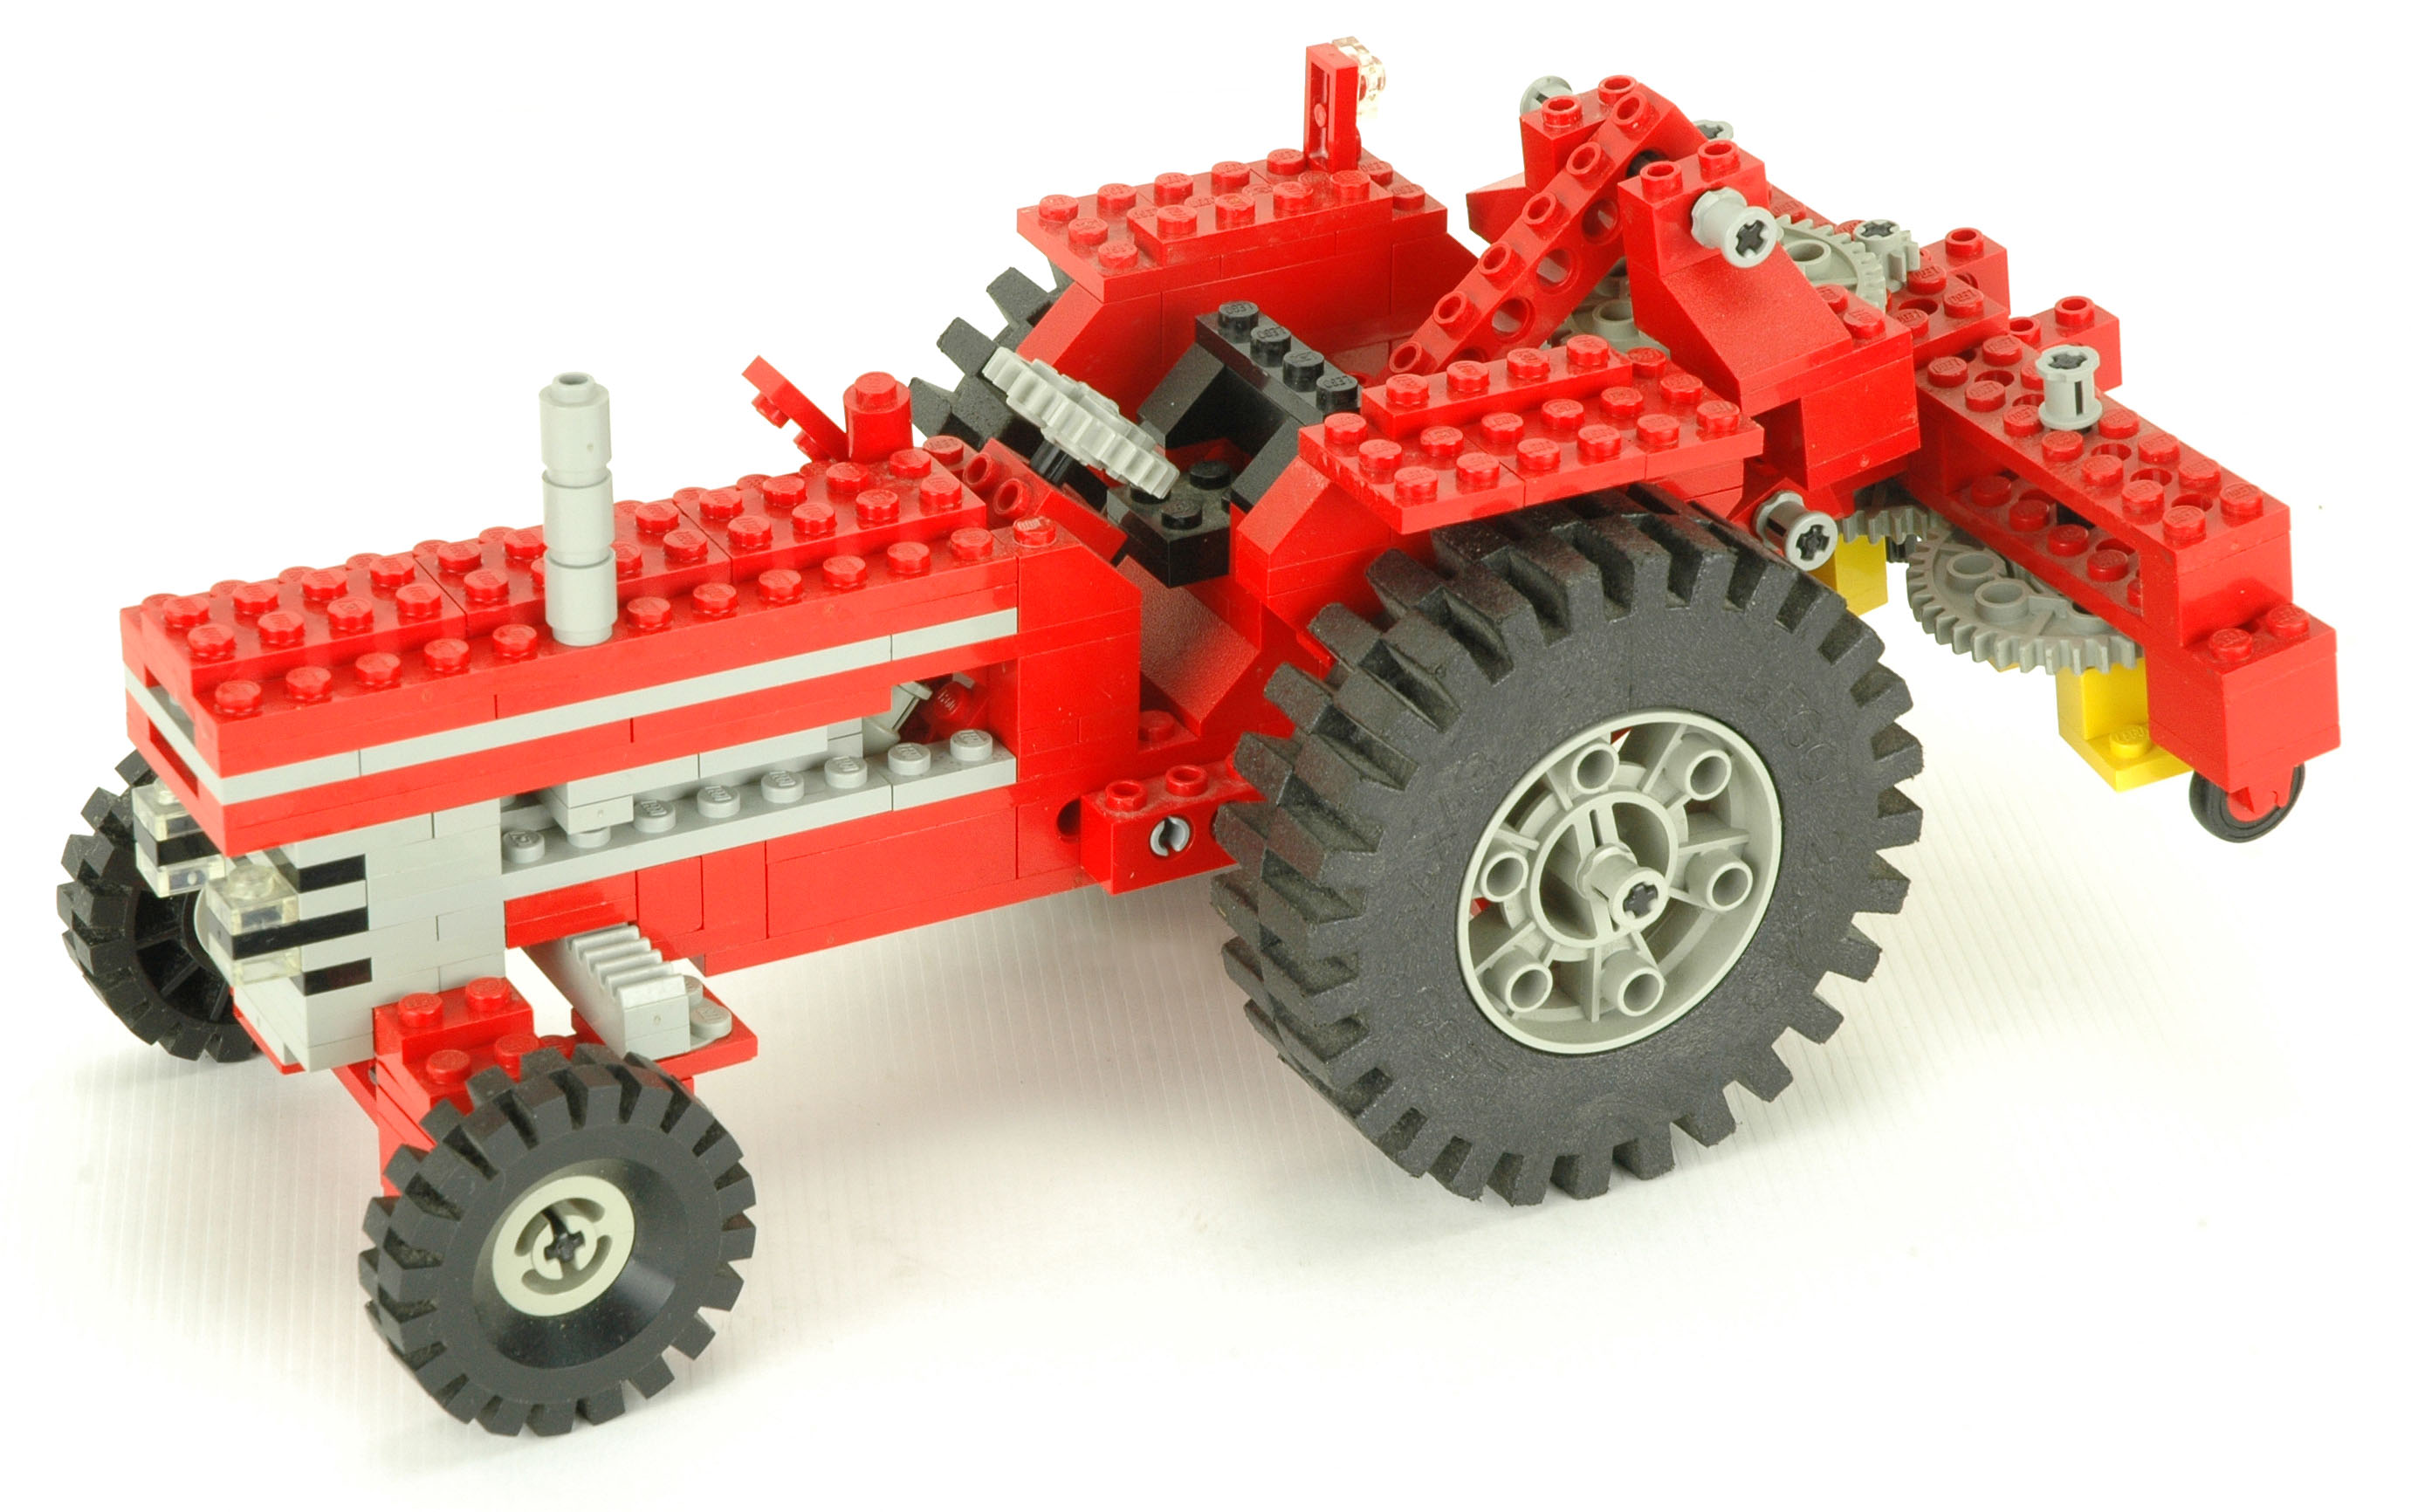
\includegraphics[width=0.99\textwidth]{1977_851_tractor}
\end{figure}
\end{frame}

\begin{frame}[fragile]{1977: 853 Auto chassis (619 pc.)}
\begin{figure}[H]
 \centering
 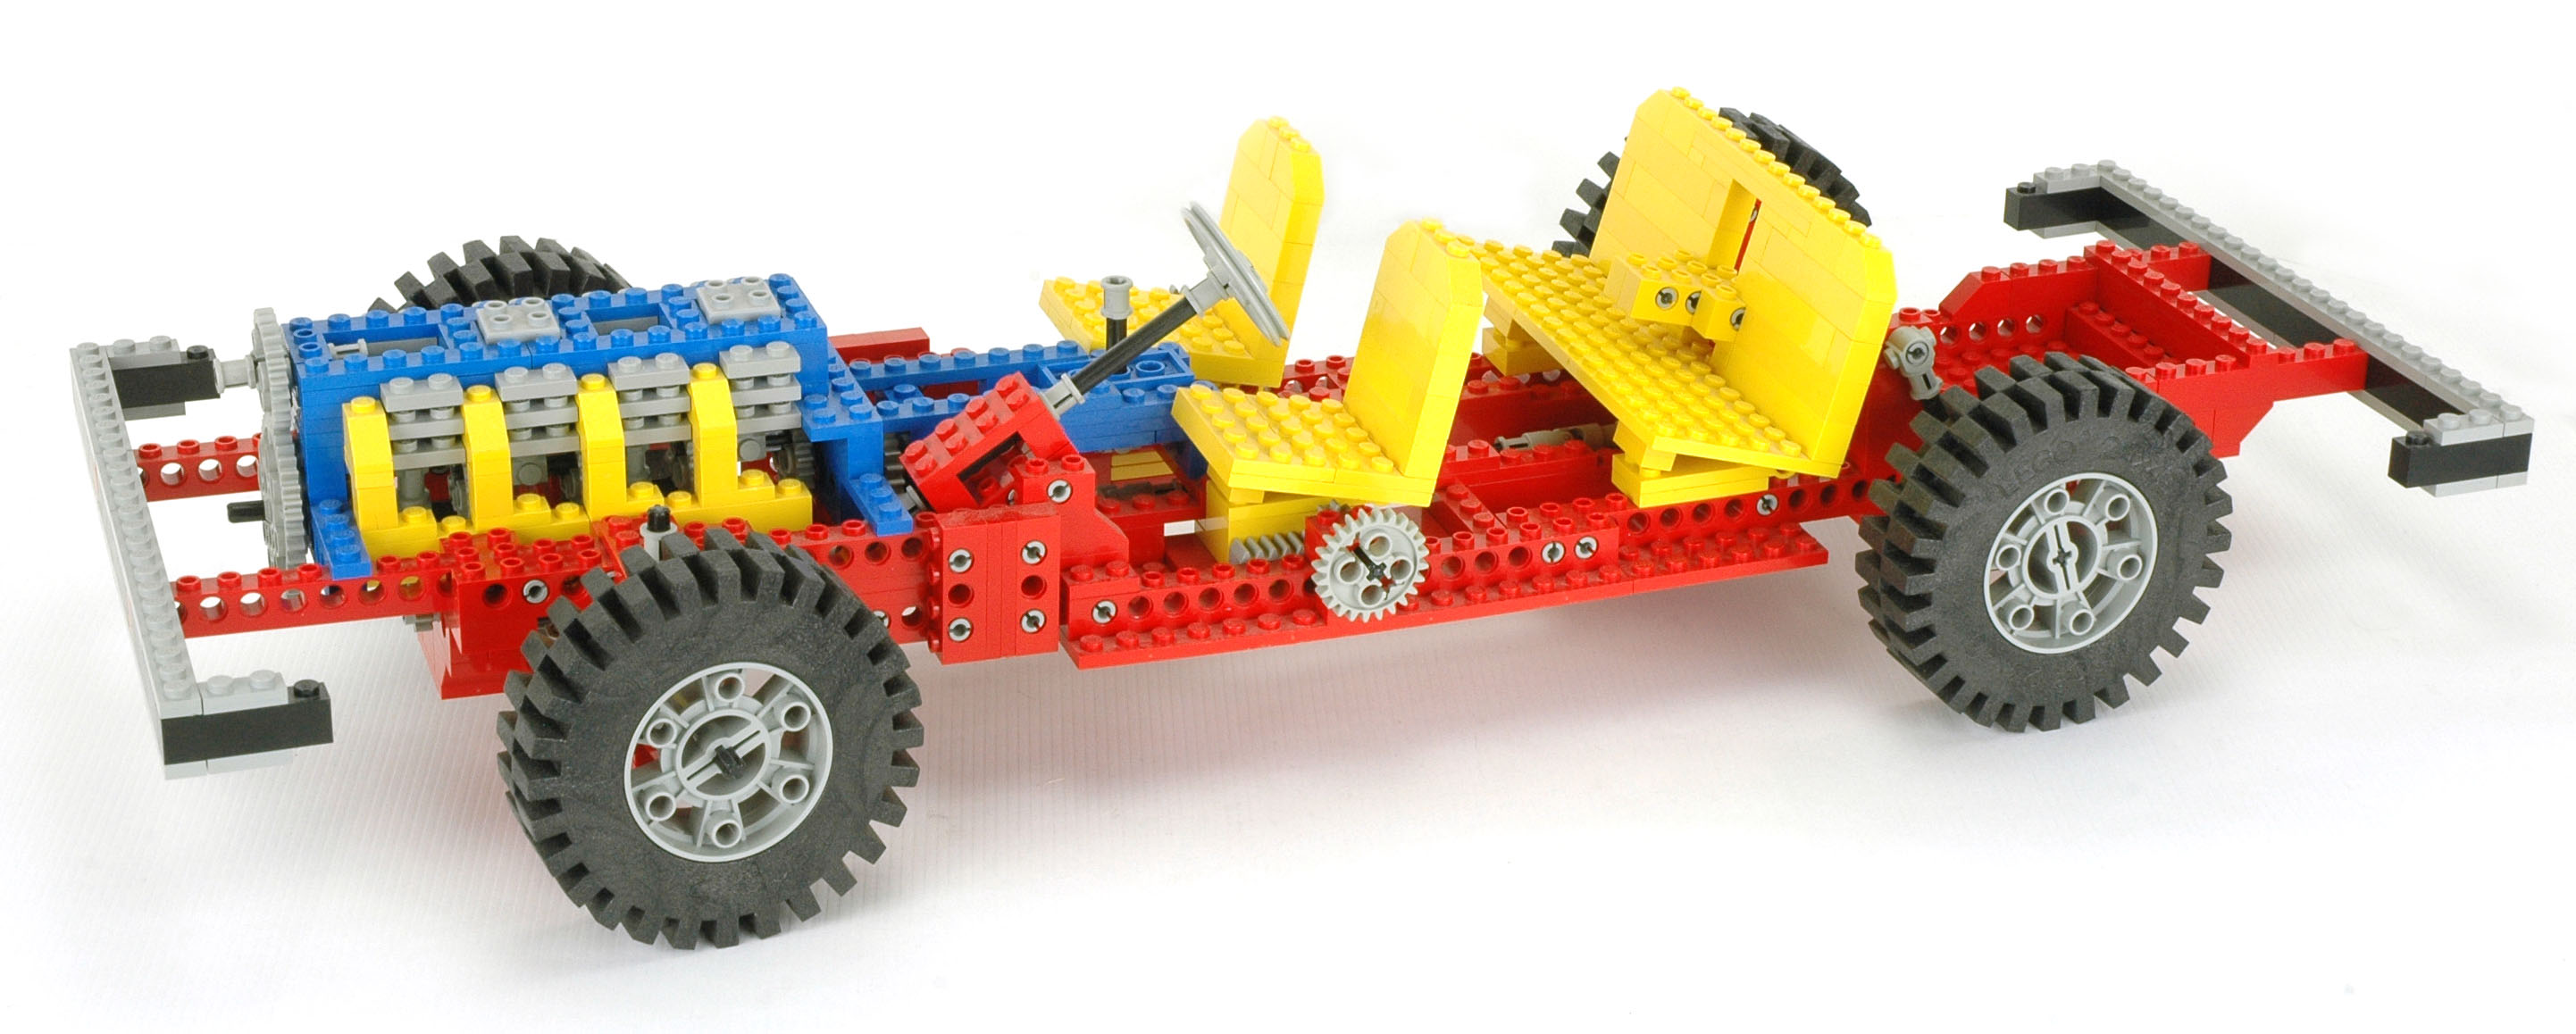
\includegraphics[width=0.99\textwidth]{1977_853_car}
\end{figure}
\end{frame}

\begin{frame}[fragile]{1978: 855 Mobile crane (520 pc.)}
\begin{figure}[H]
 \centering
 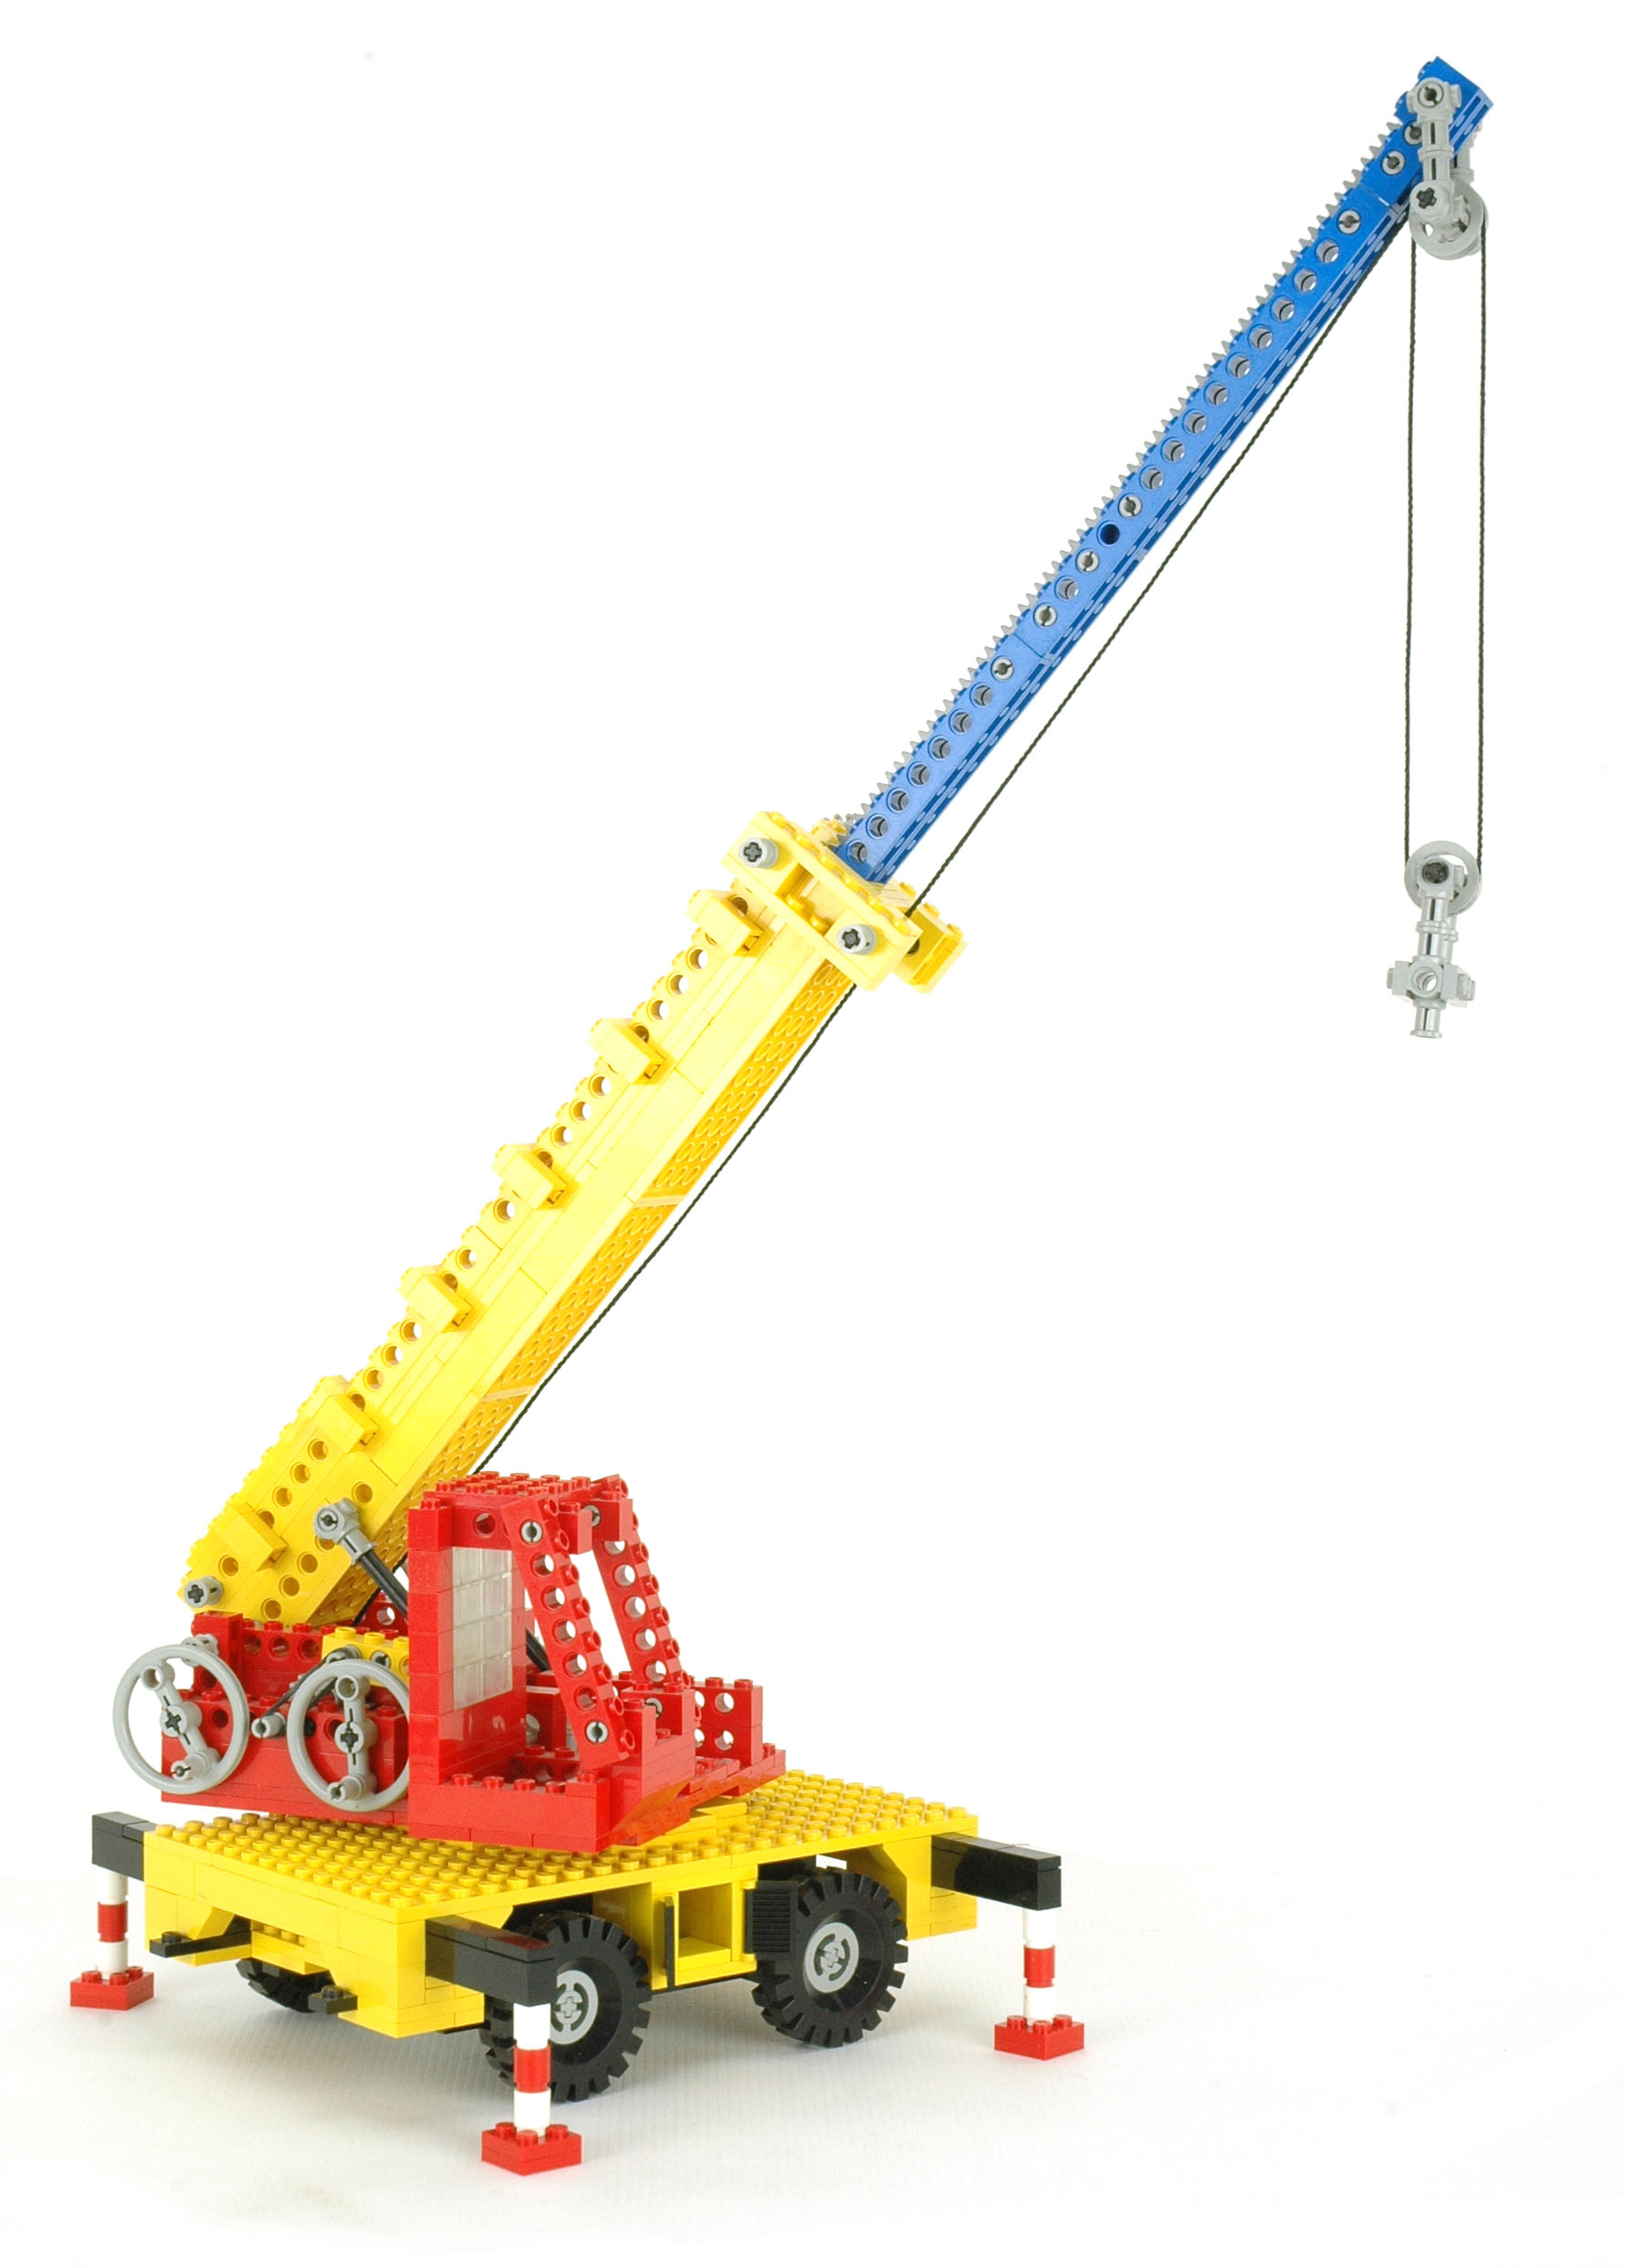
\includegraphics[height=0.7\textwidth]{1978_855_crane}
\end{figure}
\end{frame}


\begin{frame}[fragile]{1980: 8860 Auto chassis (669 pc.)}
\begin{figure}[H]
 \centering
 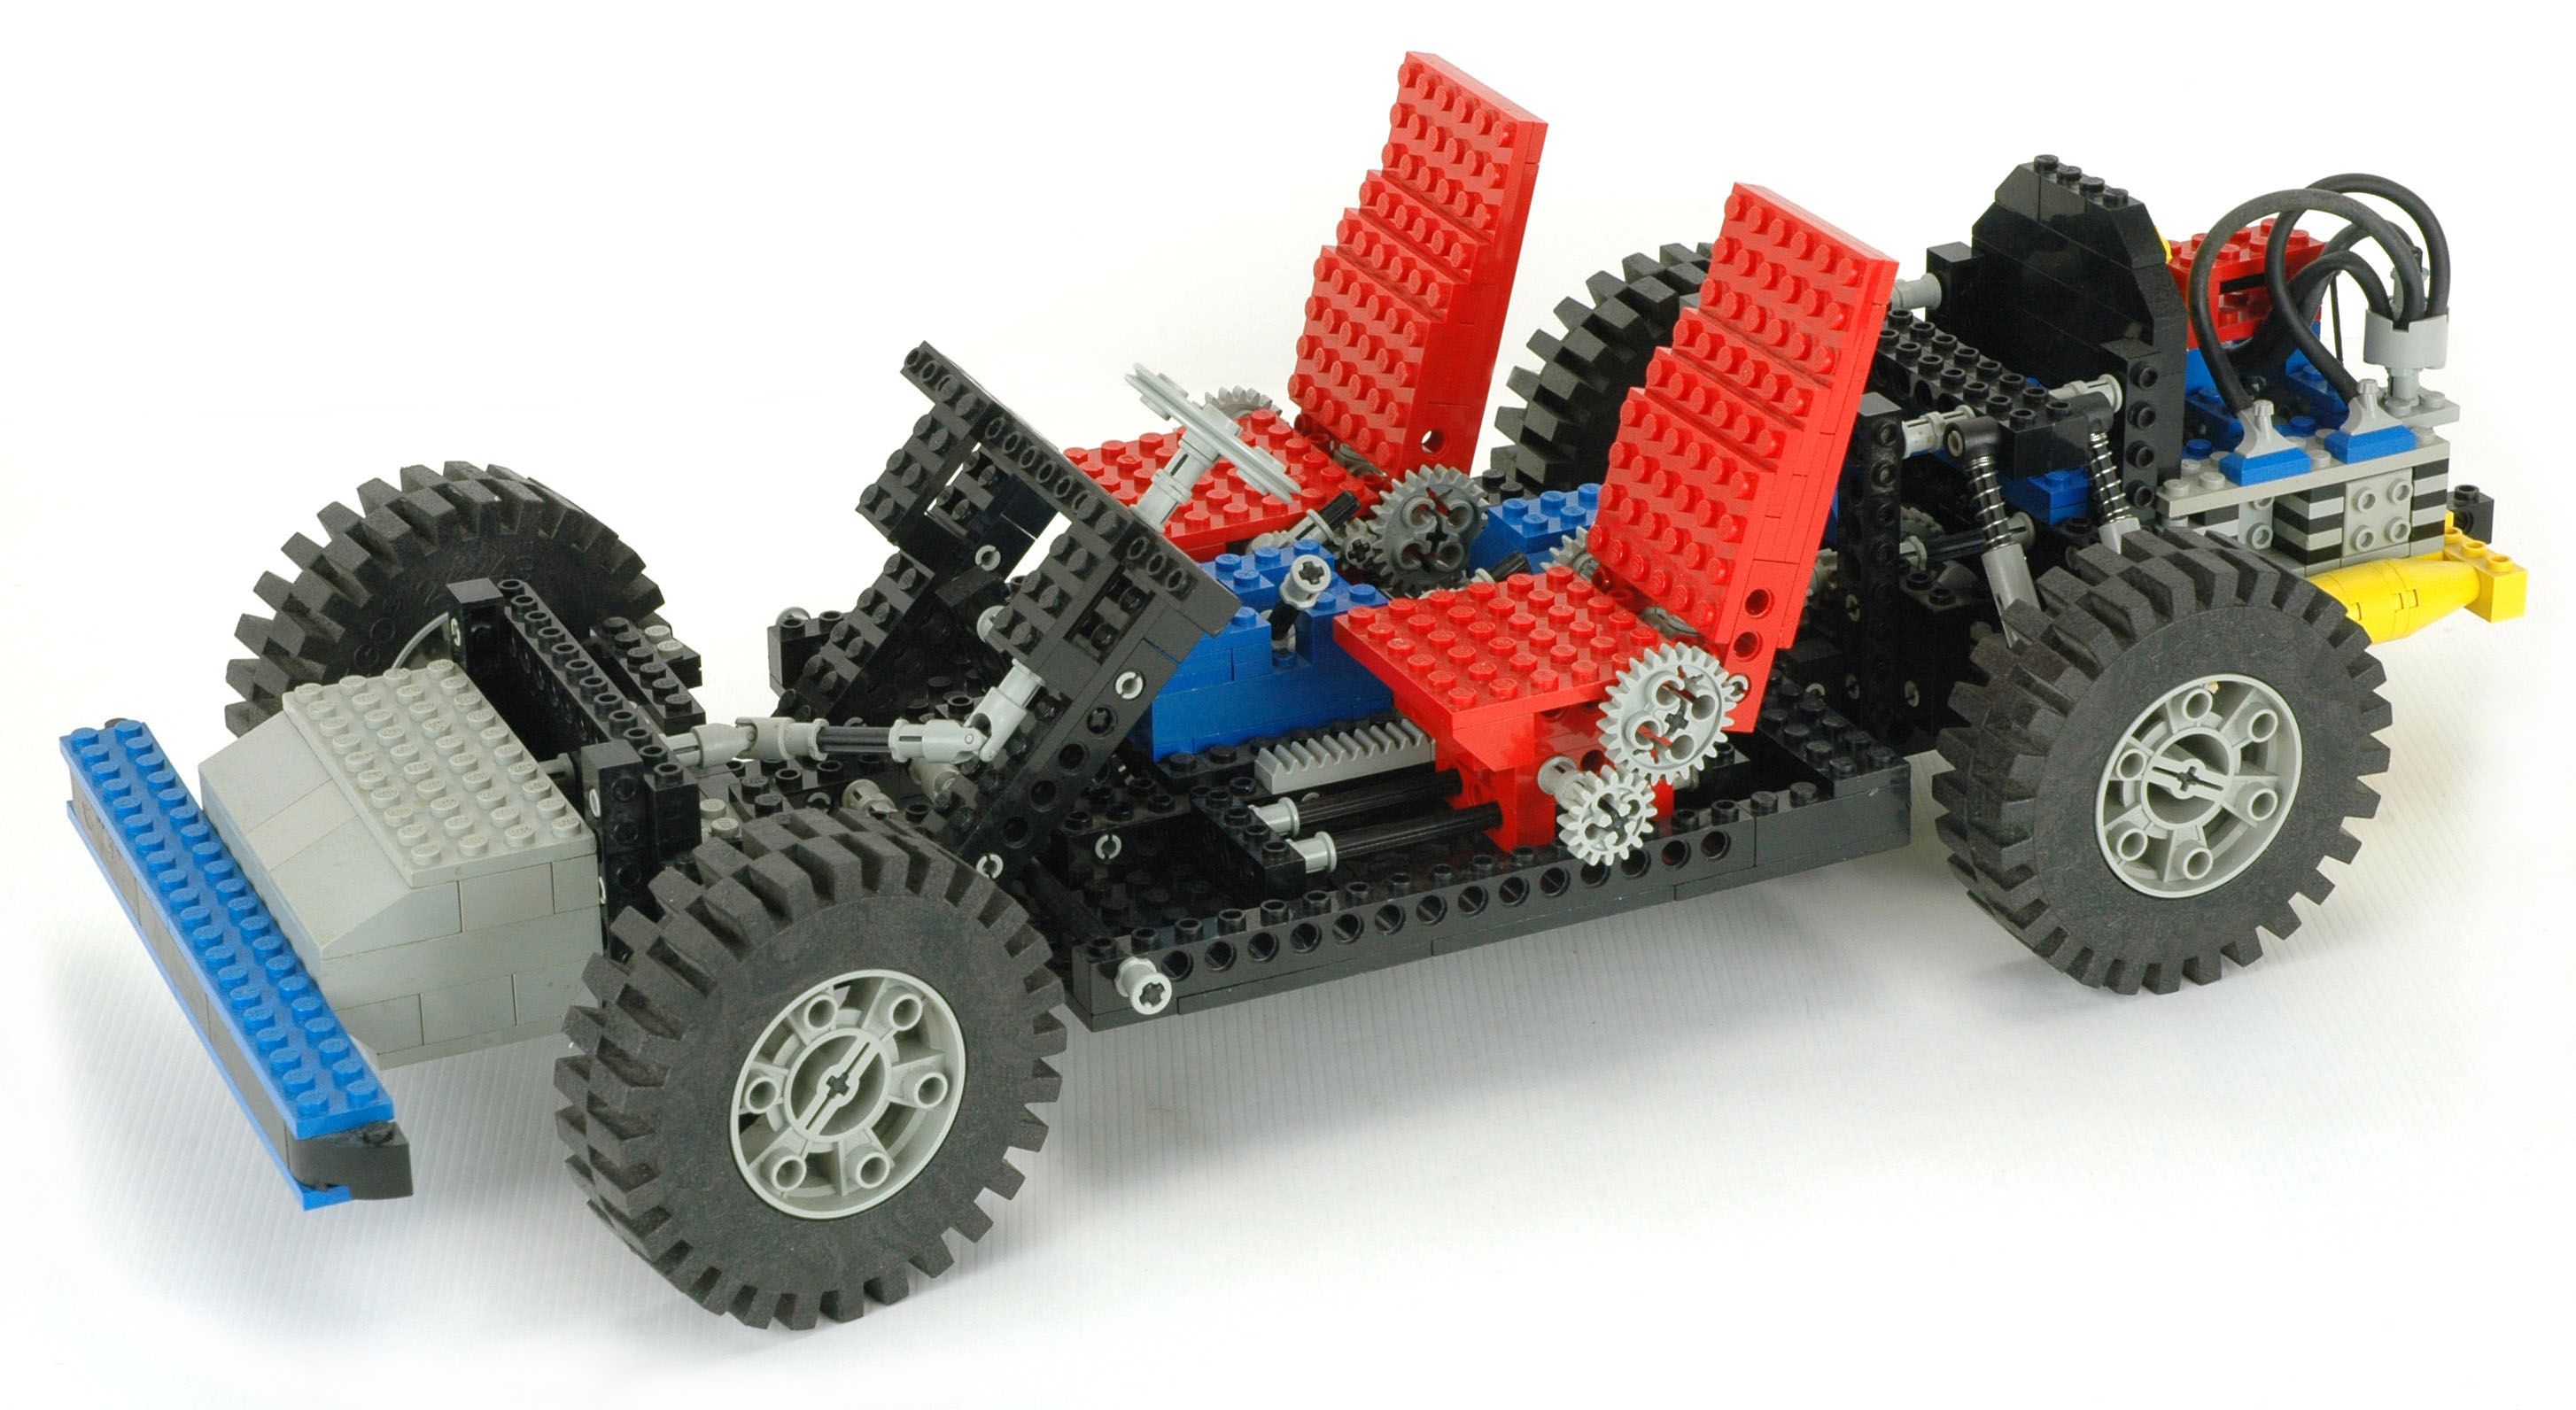
\includegraphics[width=0.99\textwidth]{1980_8860_car.jpg}
\end{figure}
\end{frame}

\begin{frame}[fragile]{Steering}
\begin{figure}[H]
 \centering
 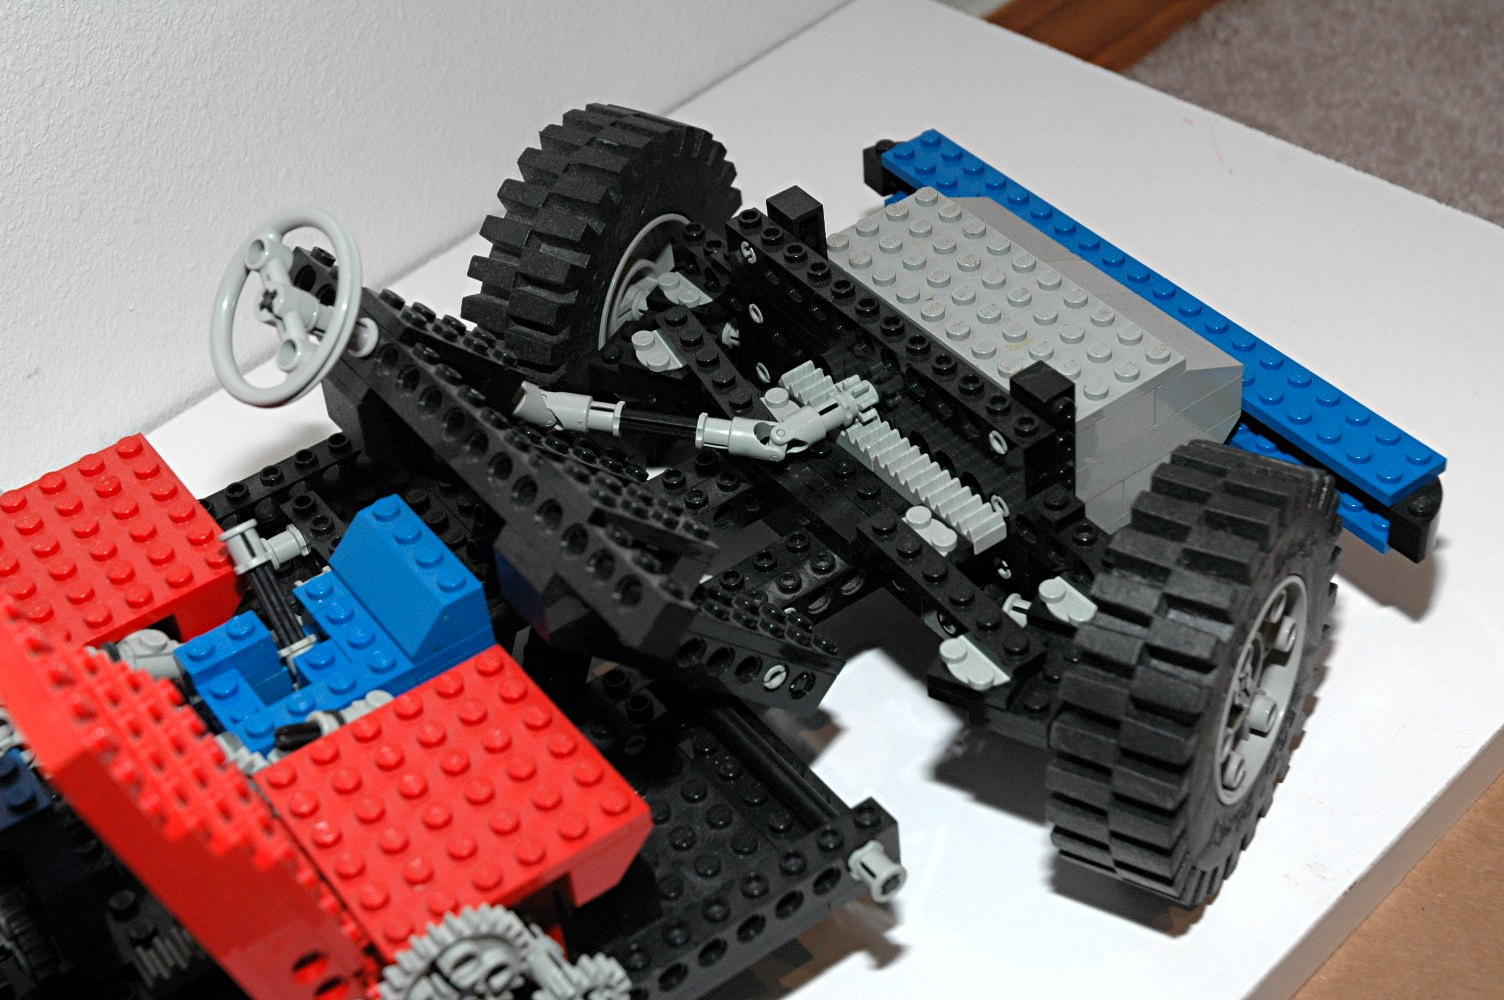
\includegraphics[trim={3cm 2cm 0 0},clip,width=0.9\textwidth]{1980_8860_steering.jpg}
\end{figure}
\end{frame}

\begin{frame}[fragile]{Suspension}
\begin{figure}[H]
 \centering
 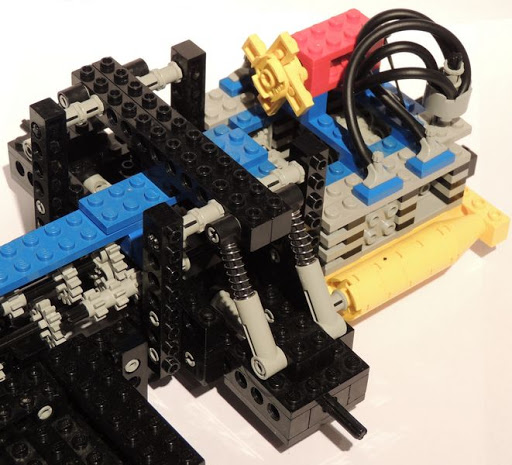
\includegraphics[width=0.7\textwidth]{1980_8860_suspension.jpg}
\end{figure}
\end{frame}

\begin{frame}[fragile]{}
\begin{itemize}
\item[--] Steering is primitive on the 8860, but at least is an Ackerman steering linkage \vspace{3mm}
\item[--] Suspension, and later drive, is added to the steering in later models \vspace{3mm}
\item[--] Rear suspension is single wishbone, but this too soon gets revised to double \vspace{3mm}
\end{itemize}
\end{frame}




\begin{frame}[fragile]{1988: 8865 Test car (911 pc.)}
\begin{figure}[H]
 \centering
 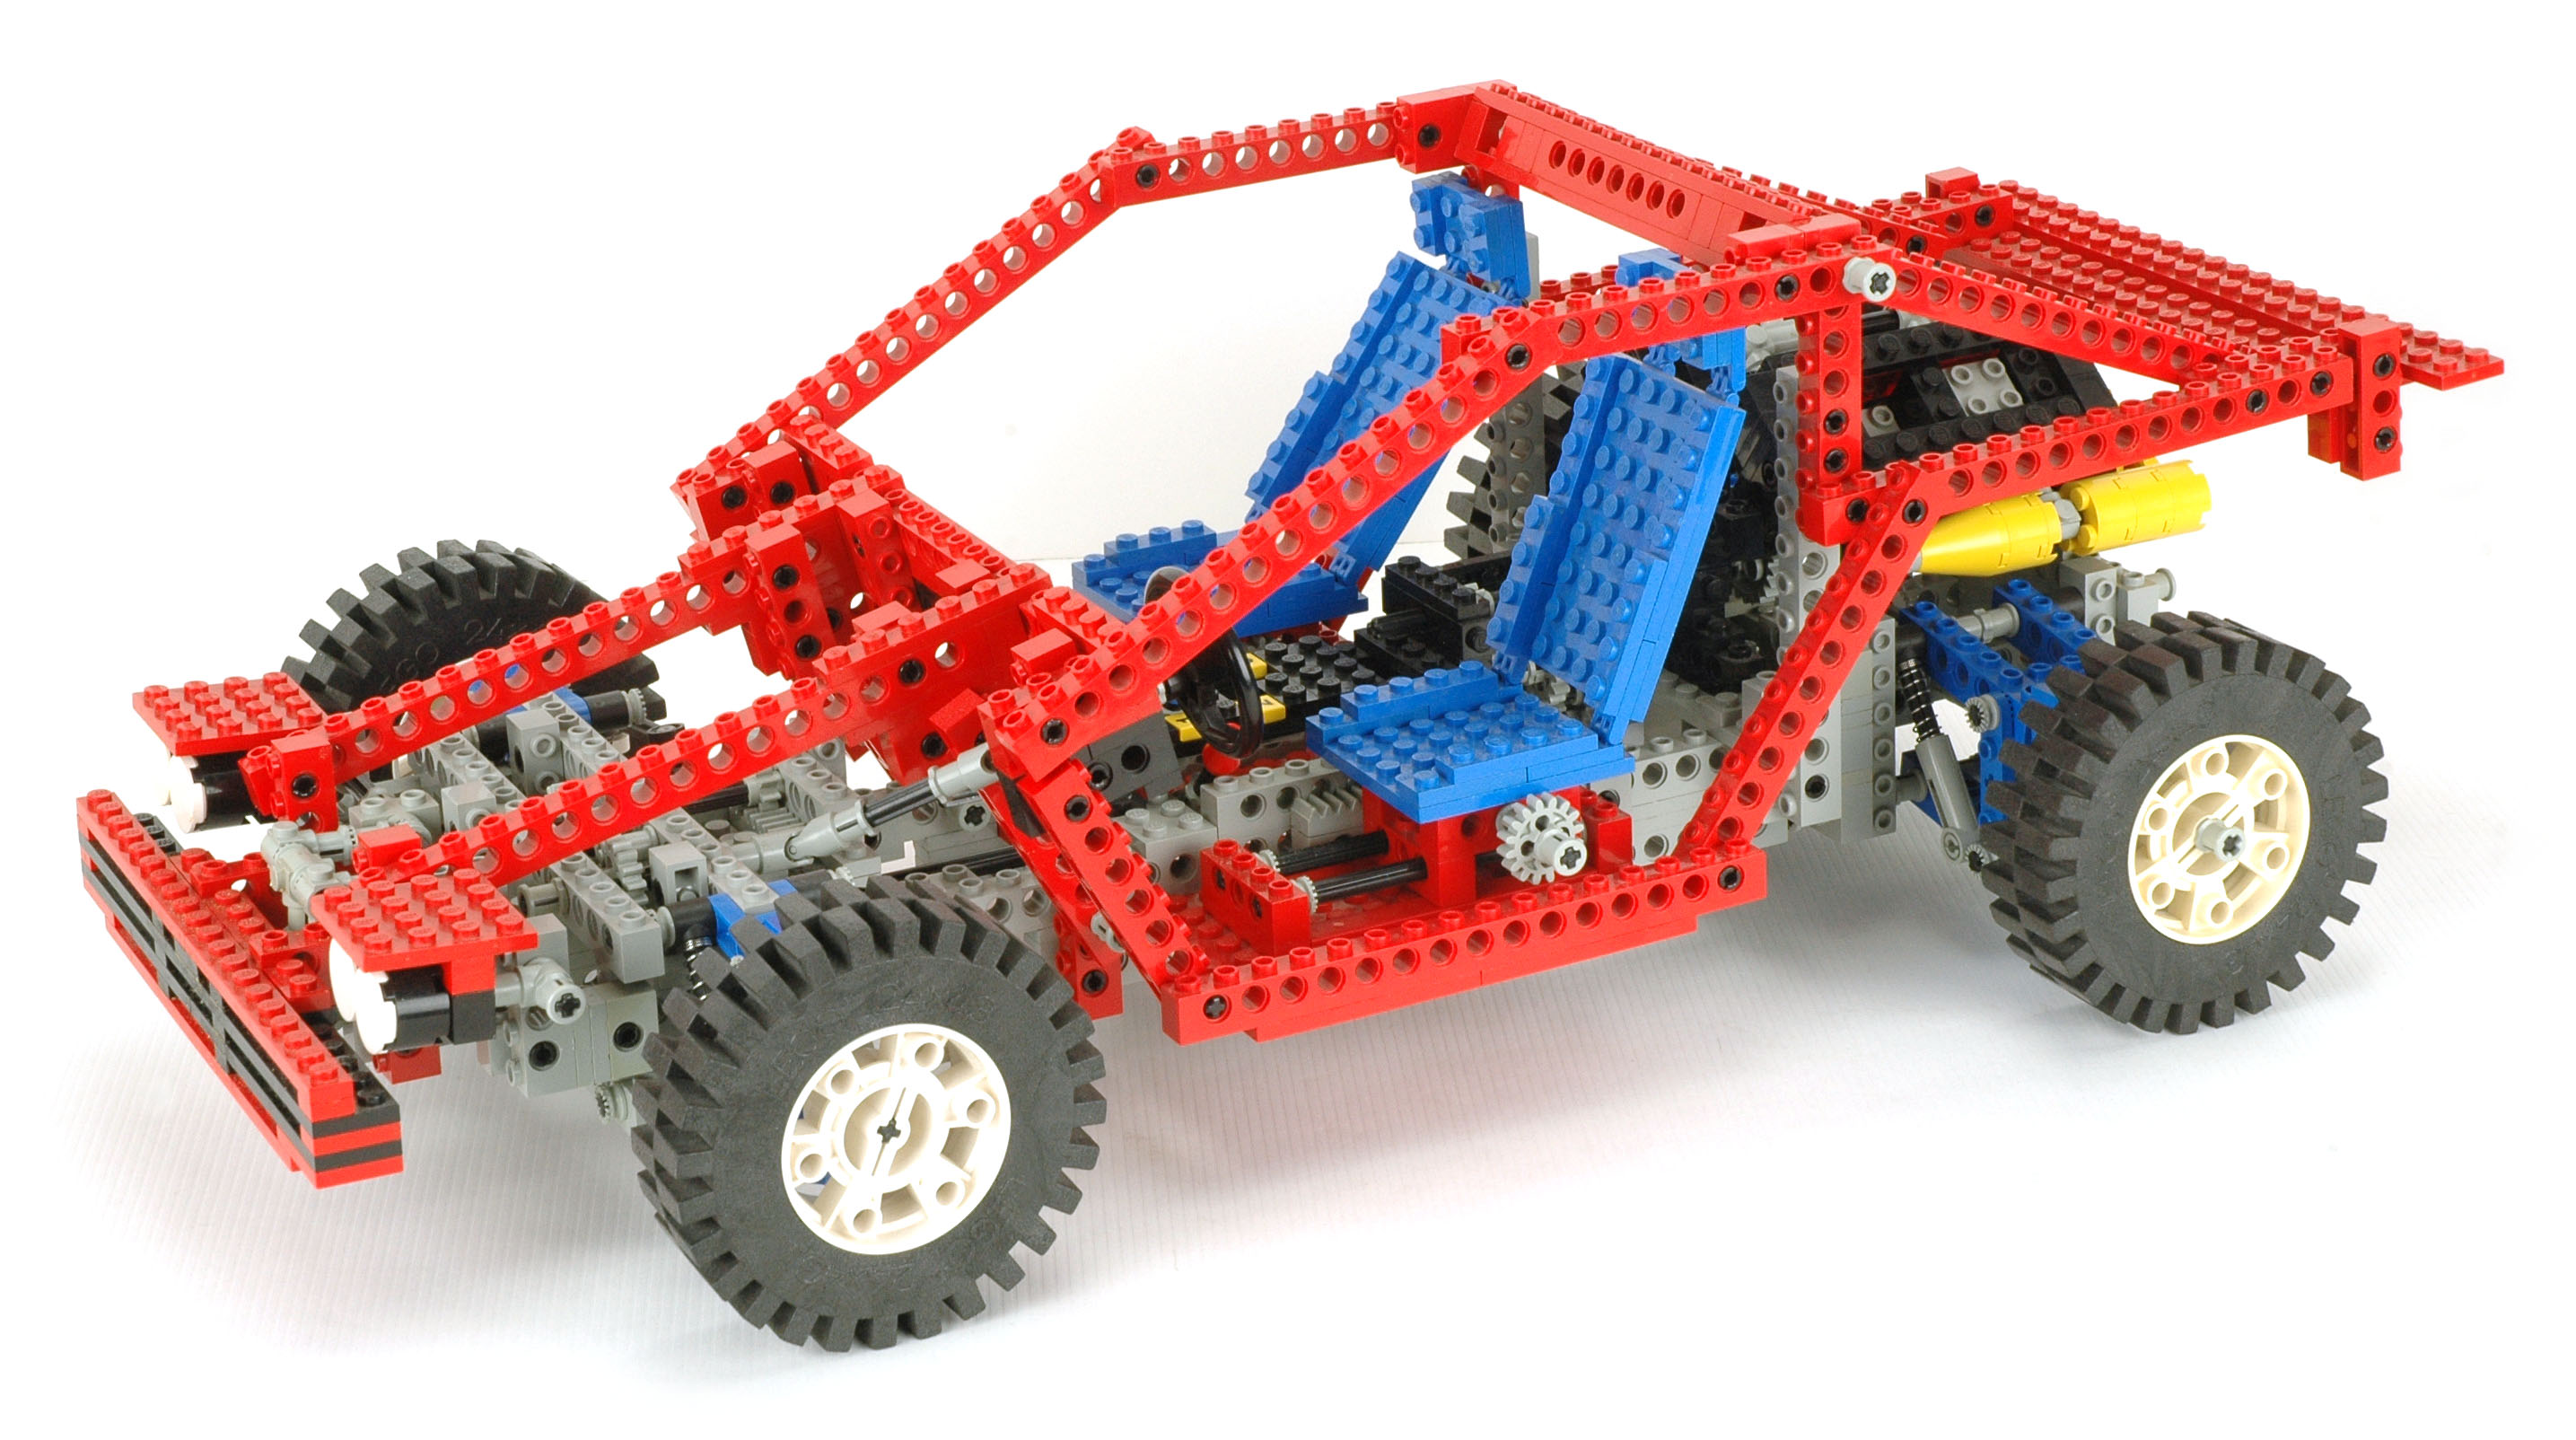
\includegraphics[width=0.99\textwidth]{1988_8865_car.jpg}
\end{figure}
\end{frame}

\begin{frame}[fragile]{Suspension}
\begin{figure}[H]
 \centering
 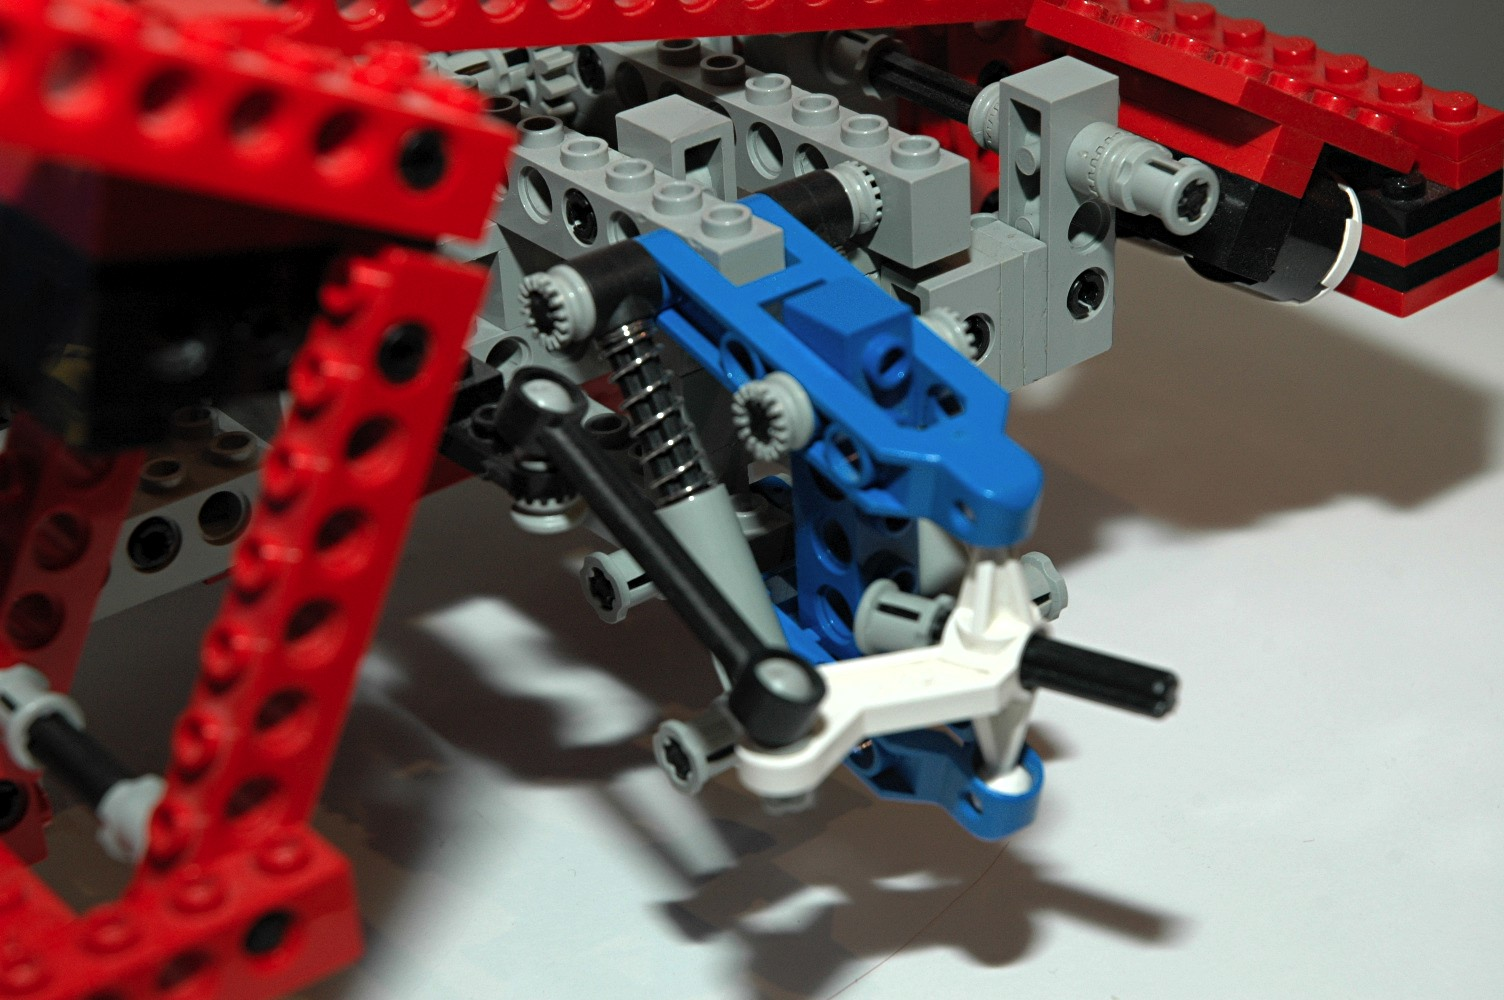
\includegraphics[width=0.99\textwidth]{1988_8865_car_front_suspension.jpg}
\end{figure}
\end{frame}

\begin{frame}[fragile]{New part. Used once.}
\begin{figure}[H]
 \centering
 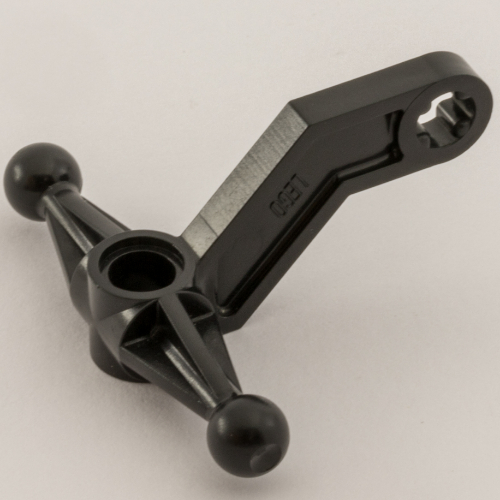
\includegraphics[width=0.6\textwidth]{1988_8865_steering_arm.jpg}
\end{figure}
\end{frame}


\begin{frame}[fragile]{Instructions}
\begin{figure}[H]
 \centering
 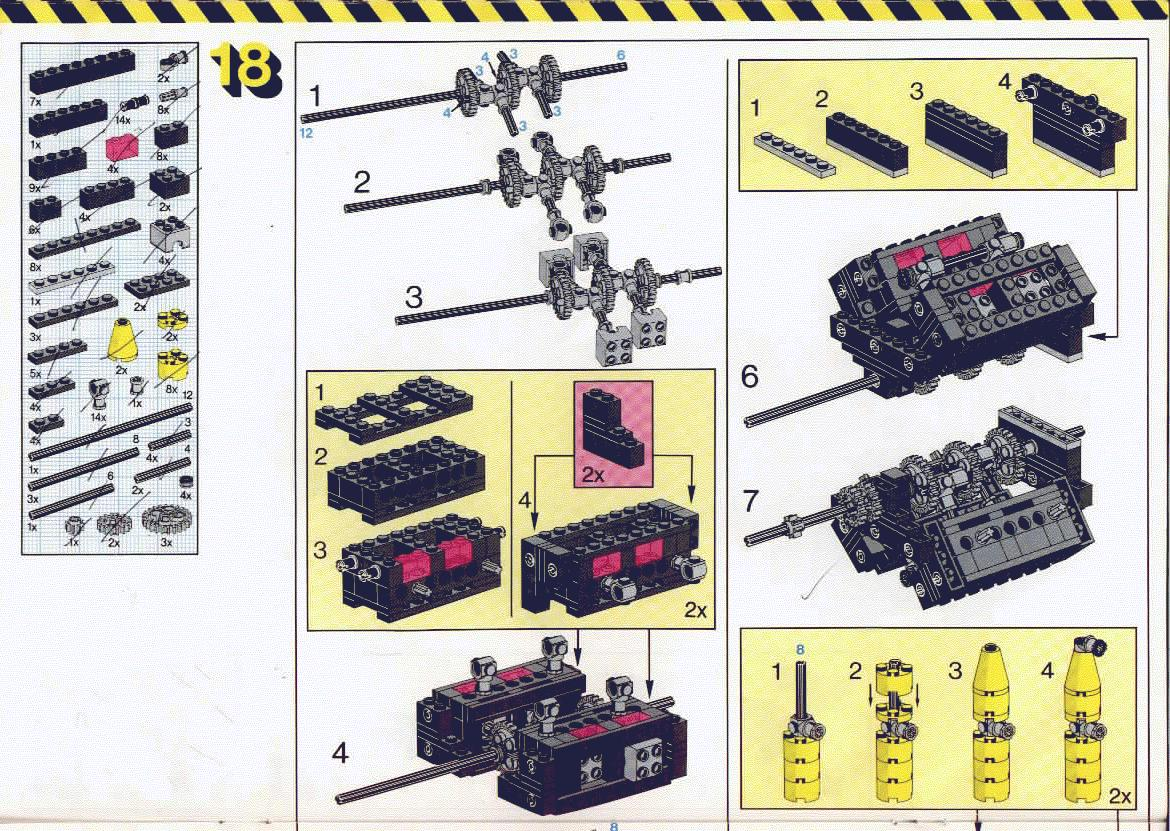
\includegraphics[width=0.85\textwidth]{1988_8865_engine_instructions.jpg}
\end{figure}
\end{frame}

\begin{frame}[fragile]{}
\begin{itemize}
\item[--] Steering and suspension are now combined, requiring new parts specially for the task \vspace{3mm}
\item[--] Instructions are quite involved: for this model there are 24 steps, and step 18 is the entire engine \vspace{3mm}
\item[--] A first attempt at offering some sort of body is made which strikes a good compromise between seeing the insides of the car and making it look like a car \vspace{3mm}
\end{itemize}
\end{frame}

\begin{frame}[fragile]{1989: 8862 Backhoe Grader (677 pc.)}
\begin{figure}[H]
 \centering
 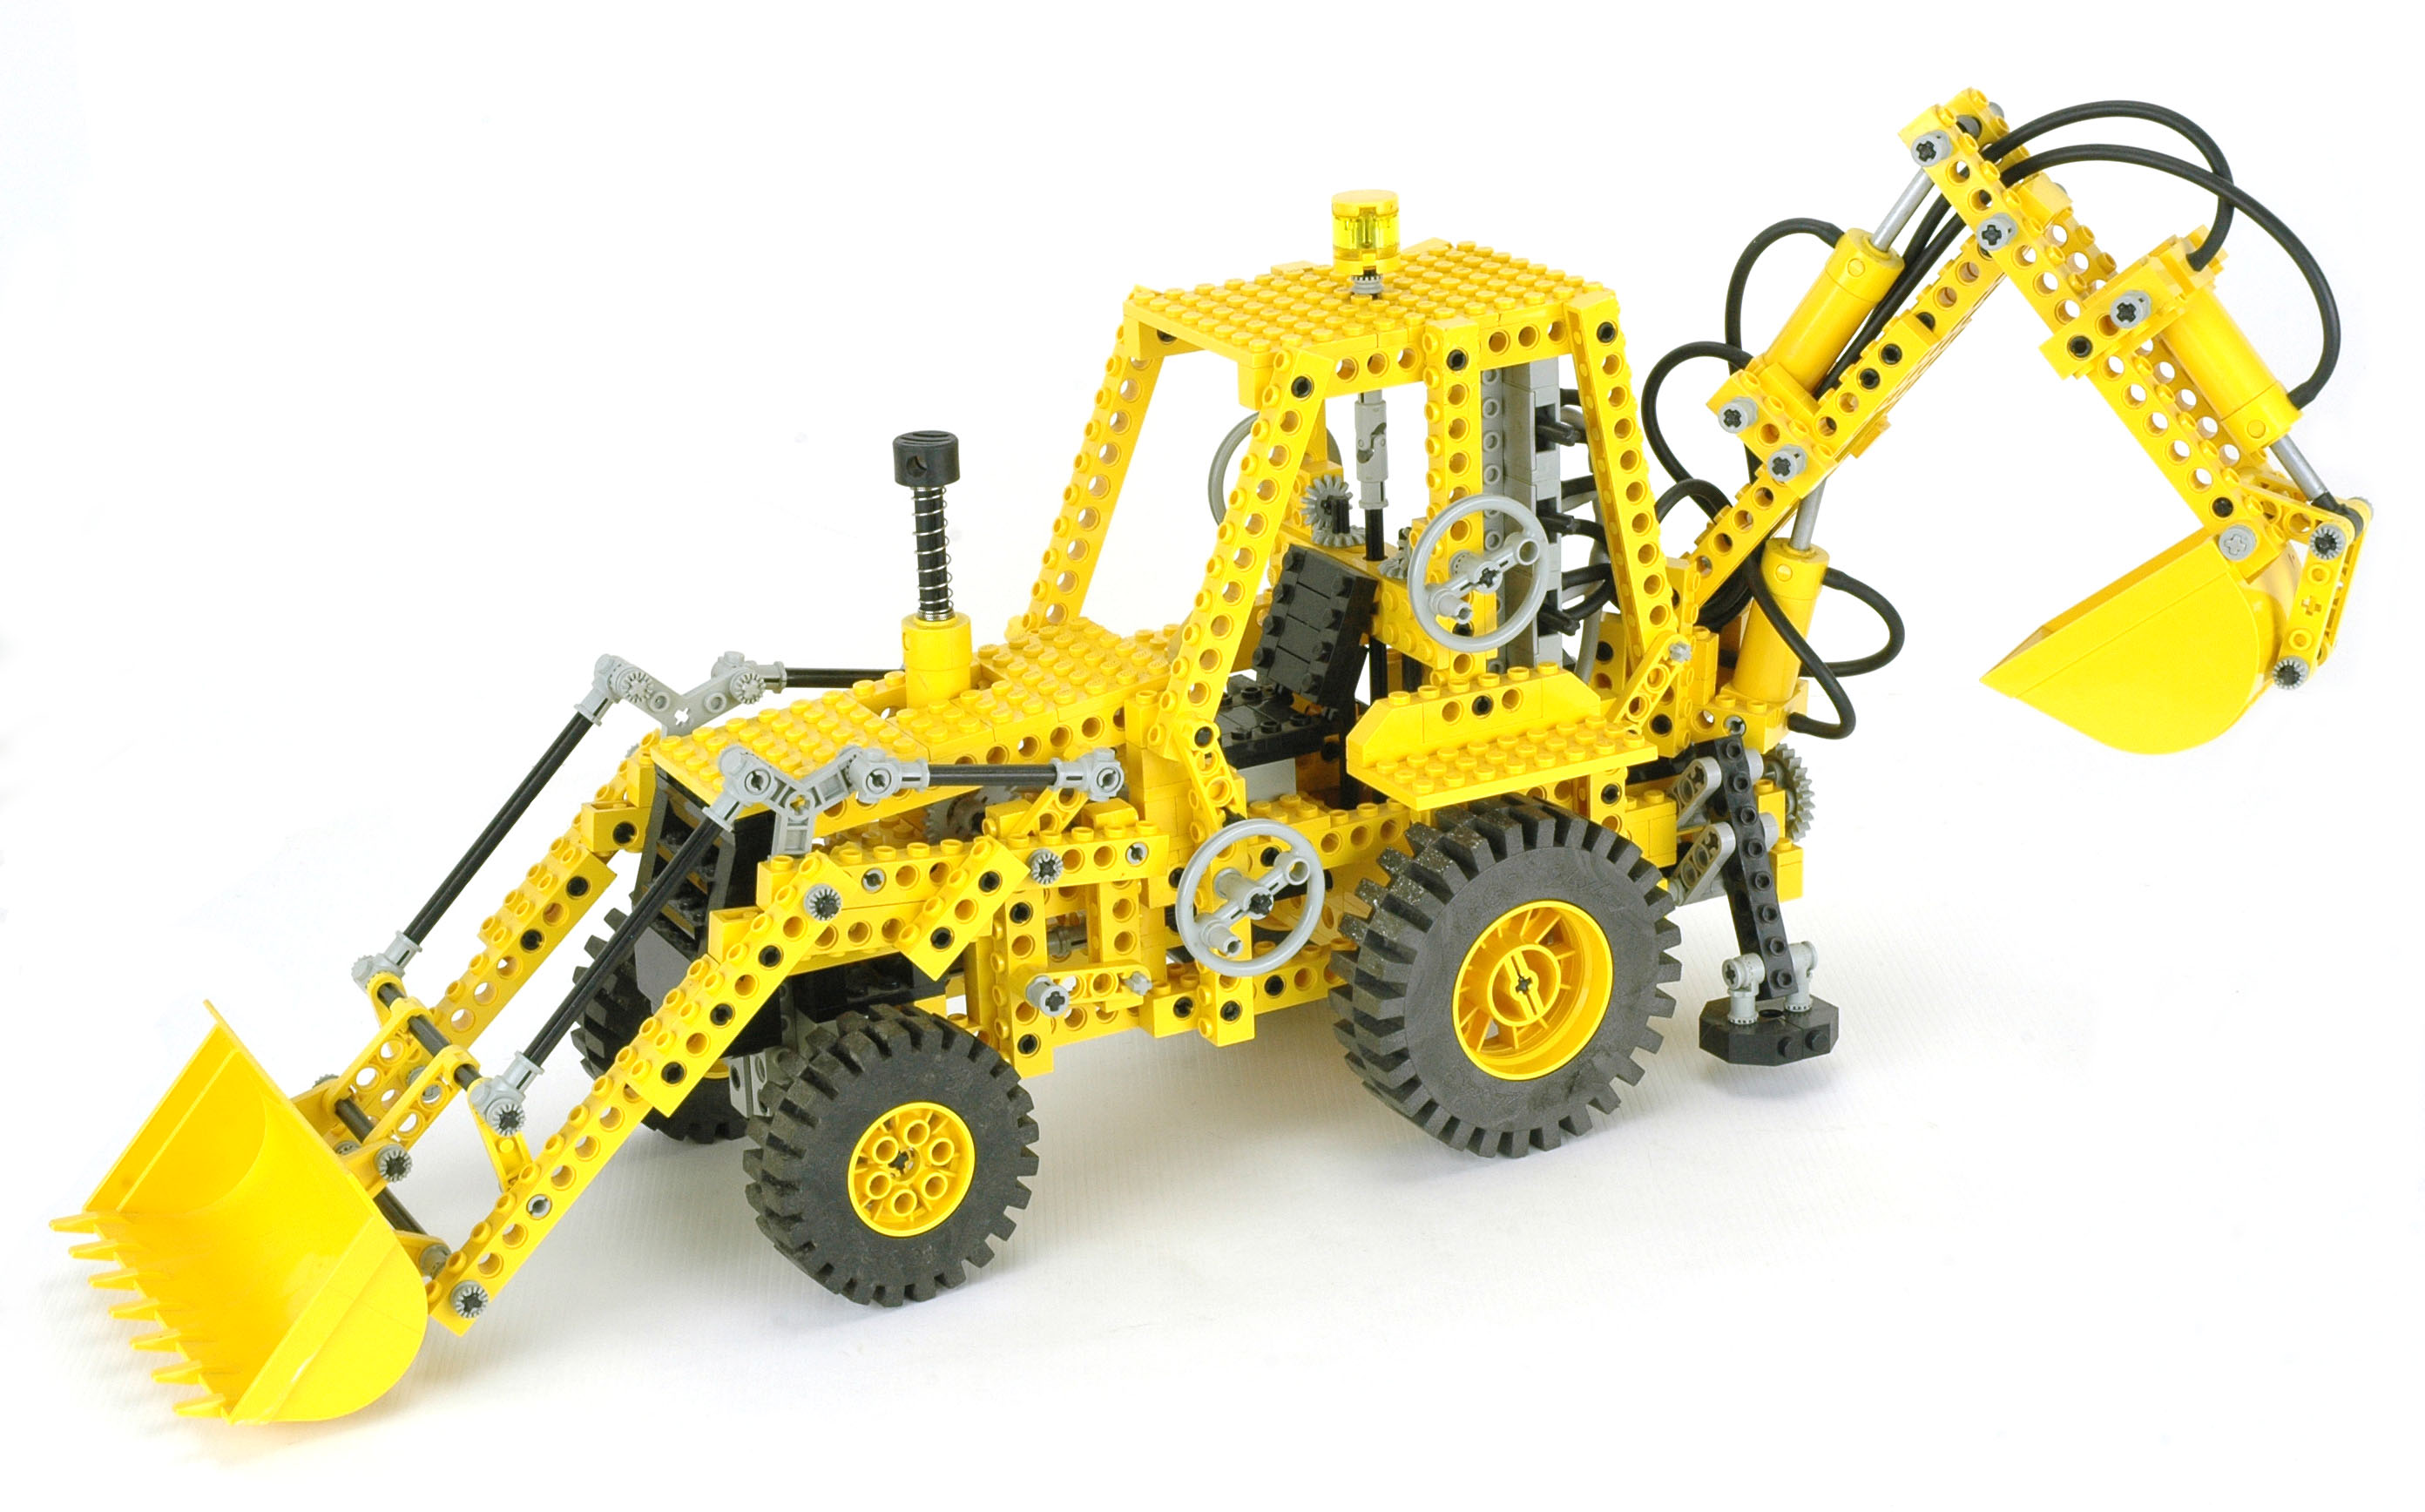
\includegraphics[width=0.99\textwidth]{1989_8862_digger.jpg}
\end{figure}
\end{frame}

\begin{frame}[fragile]{1990: homework}
\begin{figure}[H]
 \centering
 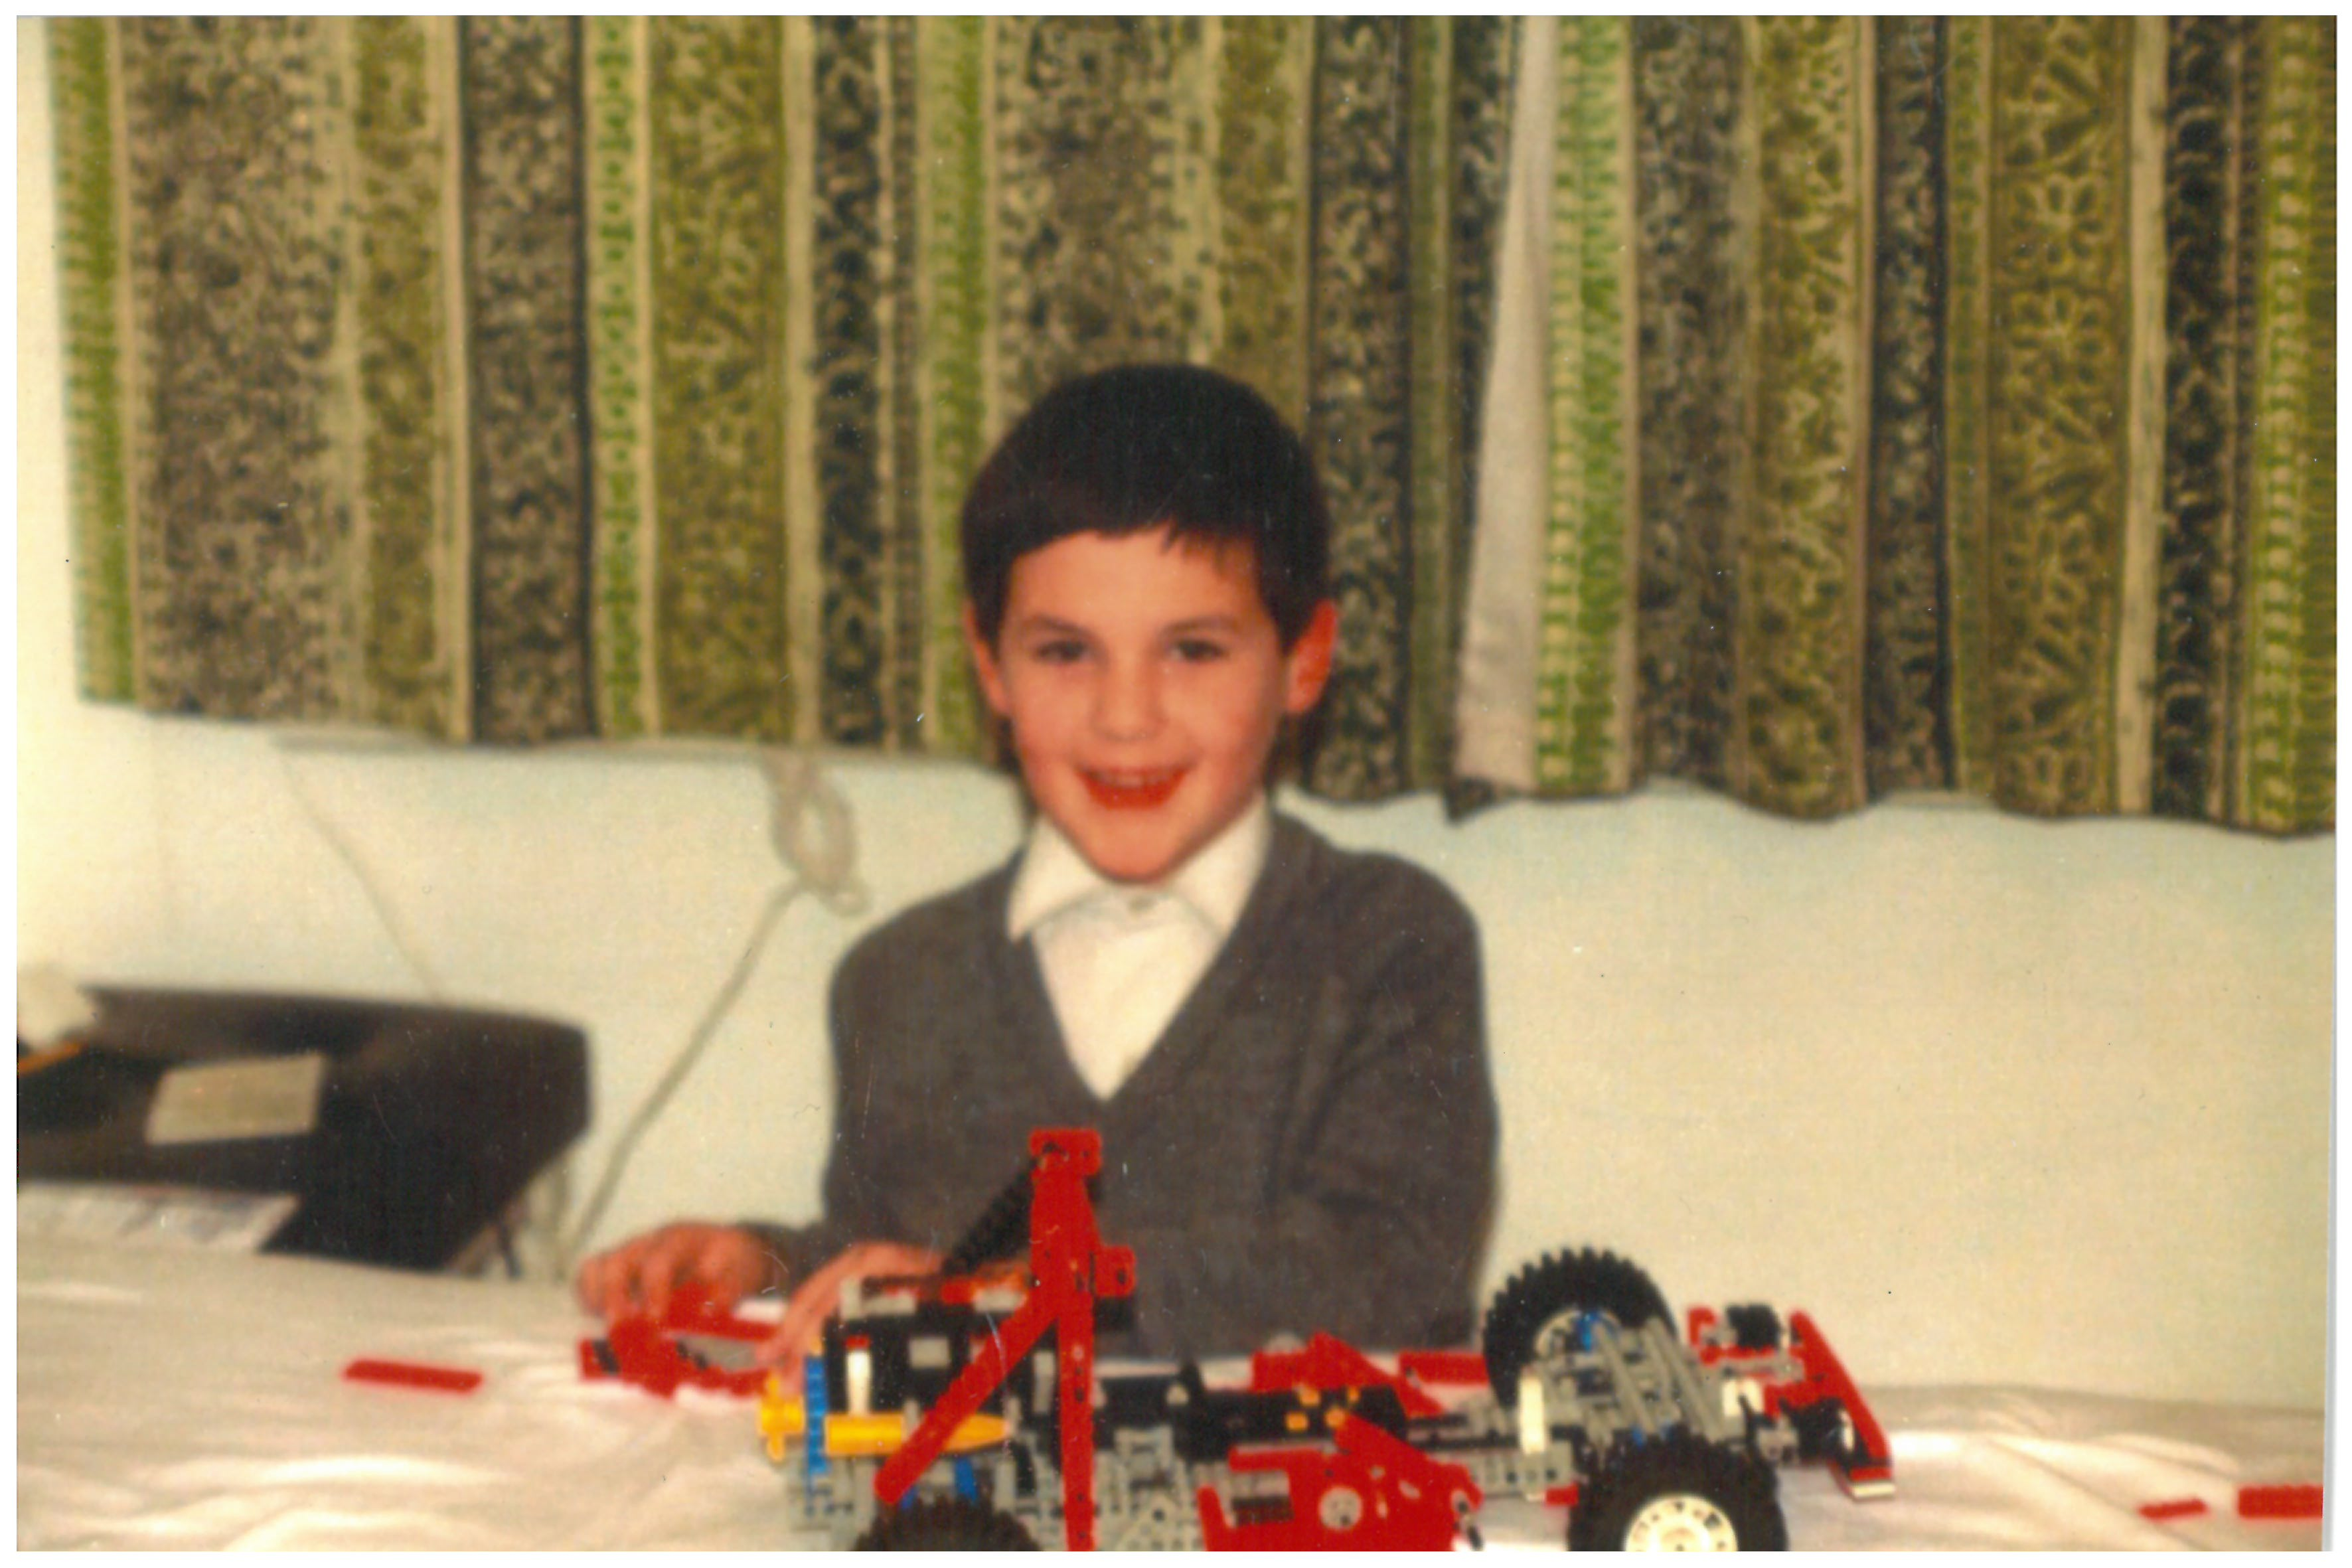
\includegraphics[width=0.9\textwidth]{1990_me.jpg}
\end{figure}
\end{frame}

\begin{frame}[fragile]{1992: 8868 Air Tech Claw Rig (969 pc.)}
\begin{figure}[H]
 \centering
 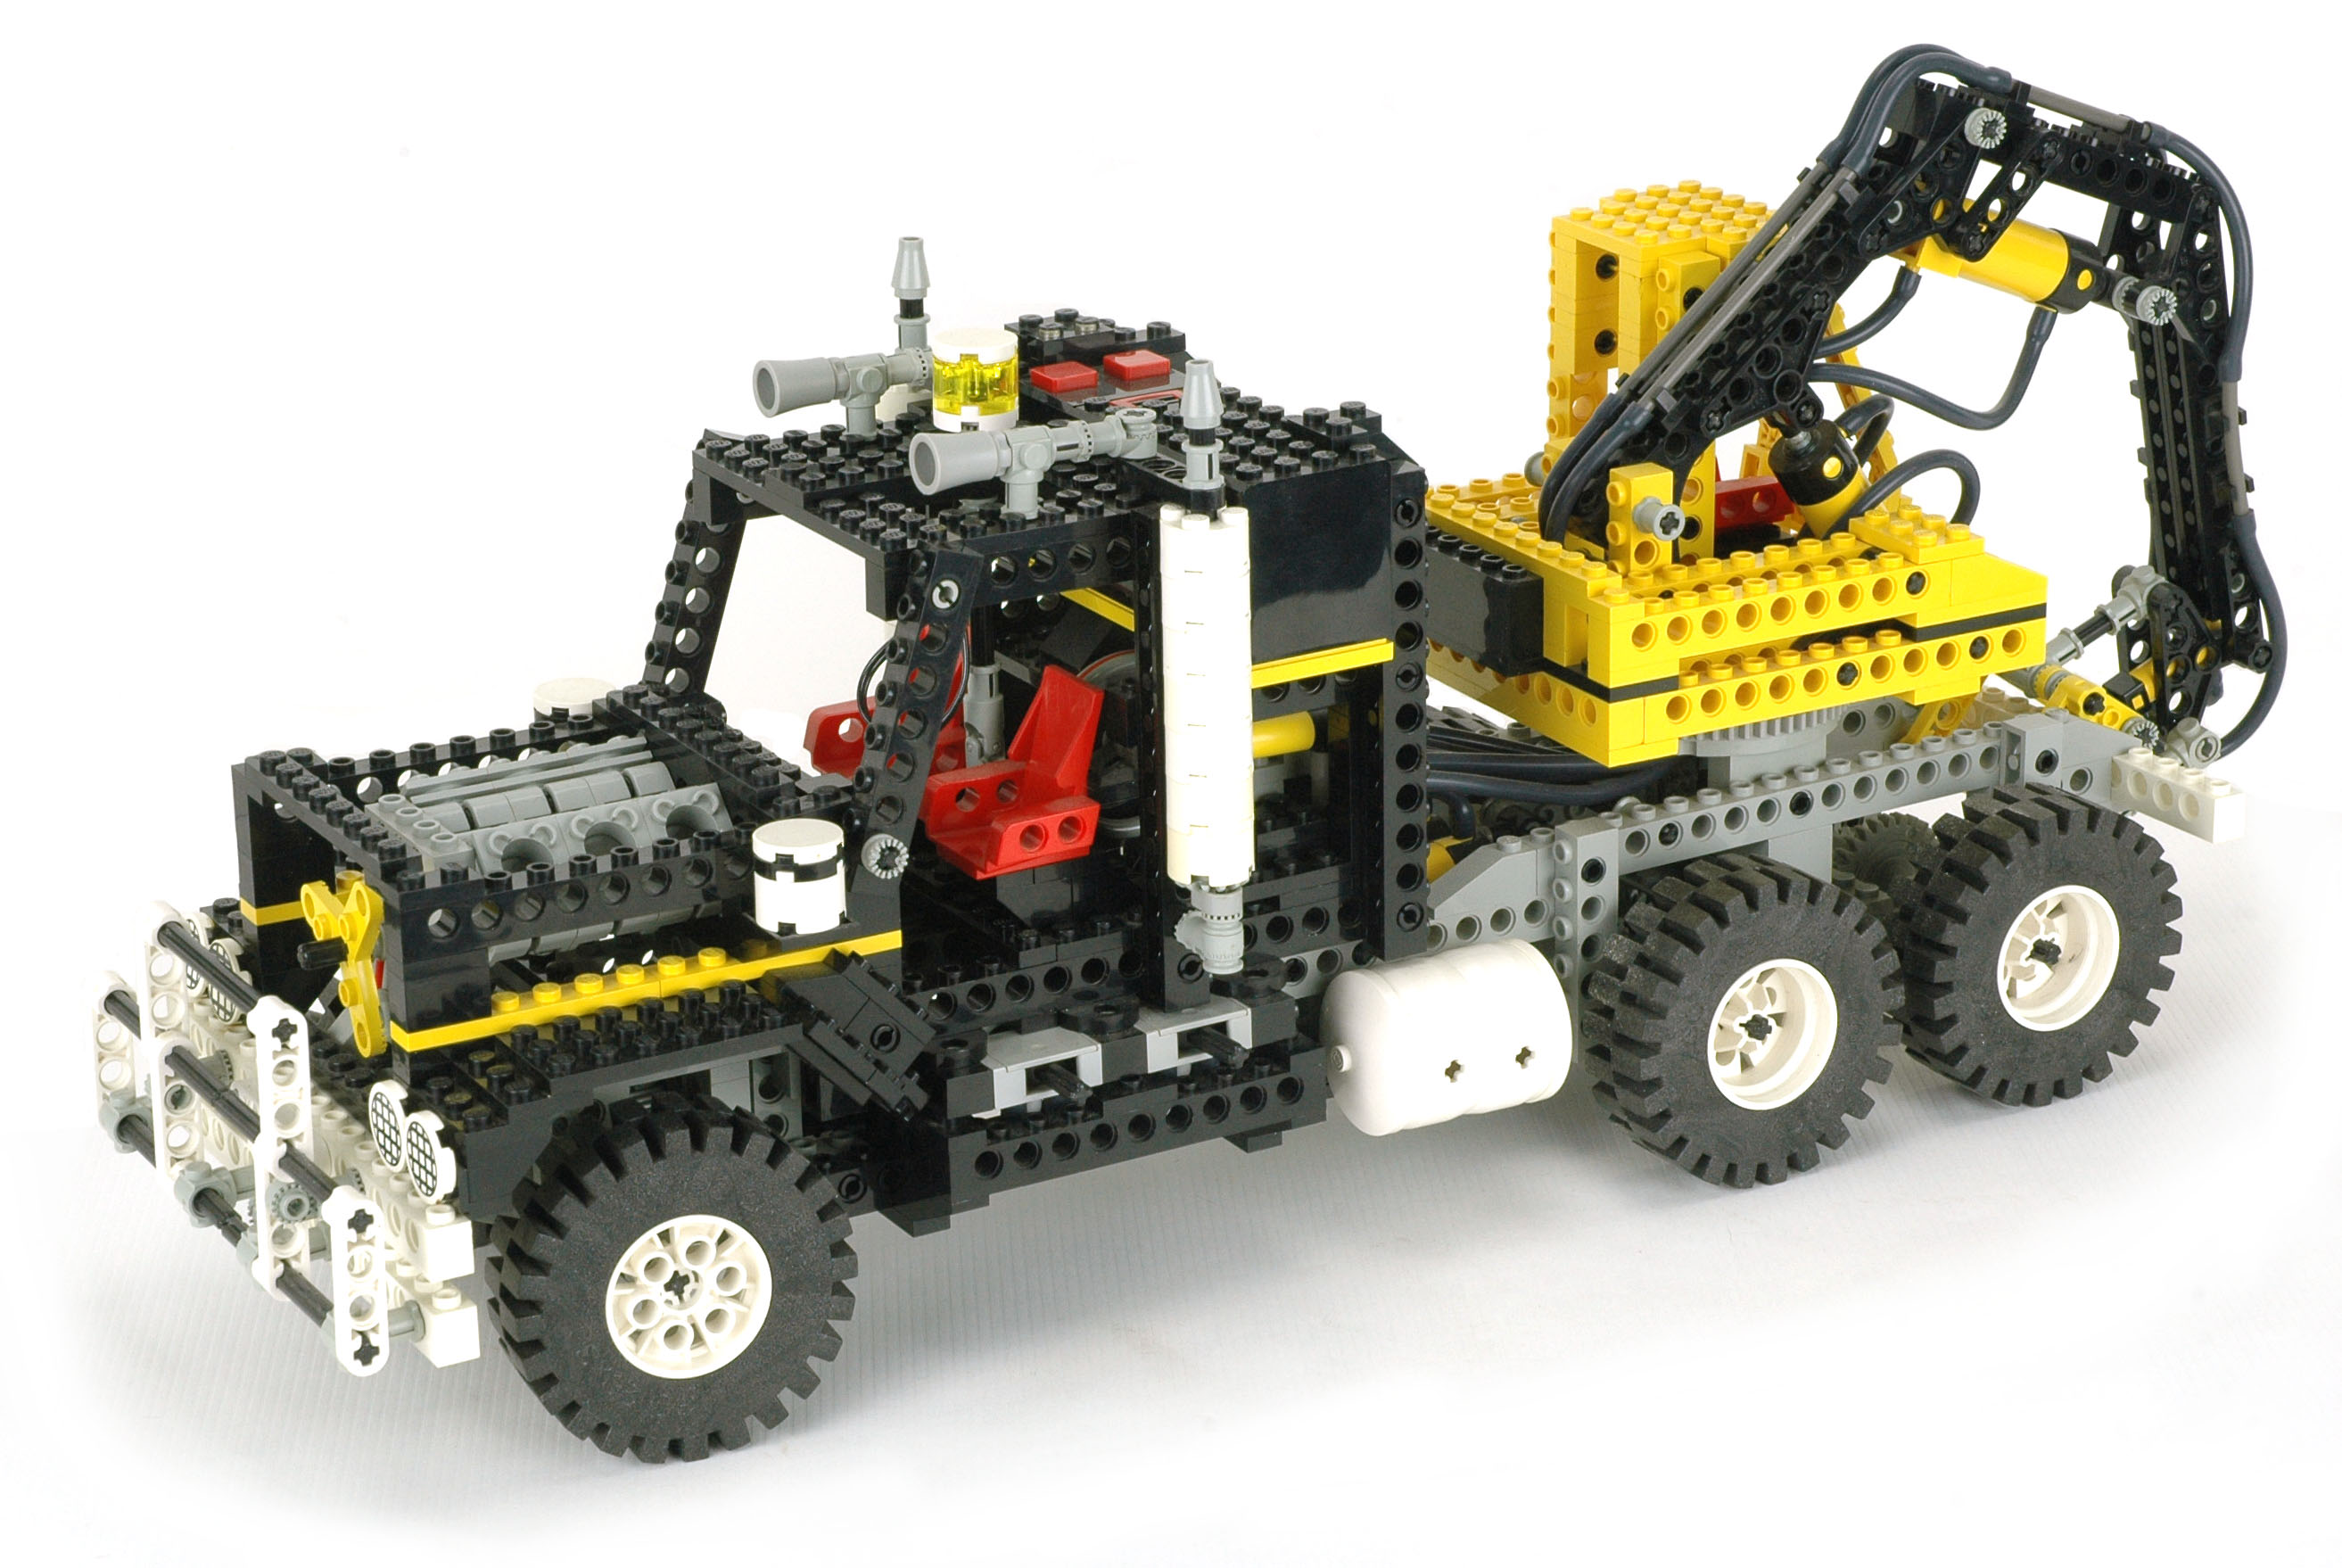
\includegraphics[width=0.99\textwidth]{1992_8868_truck.jpg}
\end{figure}
\end{frame}

\begin{frame}[fragile]{Instructions}
\begin{figure}[H]
 \centering
 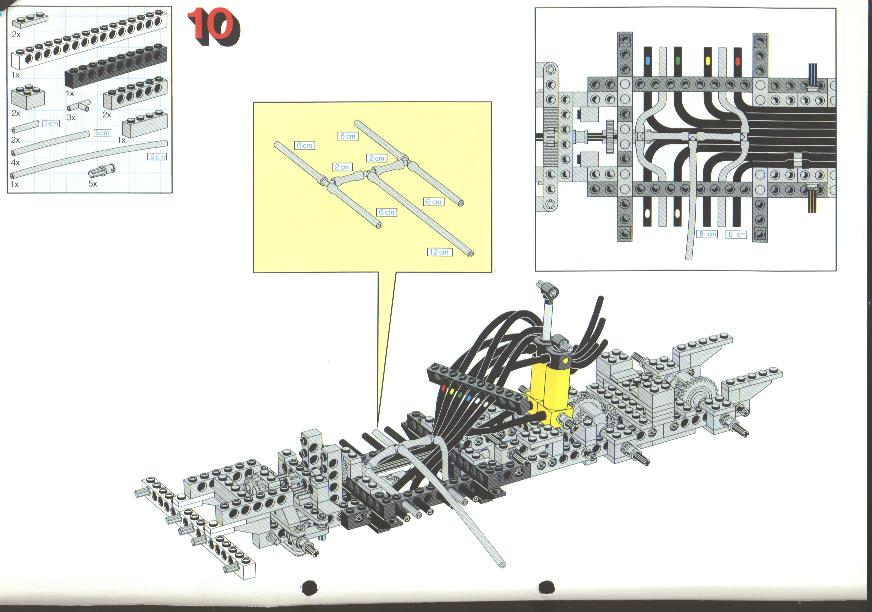
\includegraphics[width=0.85\textwidth]{1992_8868_truck_instruction_10.jpg}
\end{figure}
\end{frame}

\begin{frame}[fragile]{Pneumatics}
\begin{figure}[H]
 \centering
 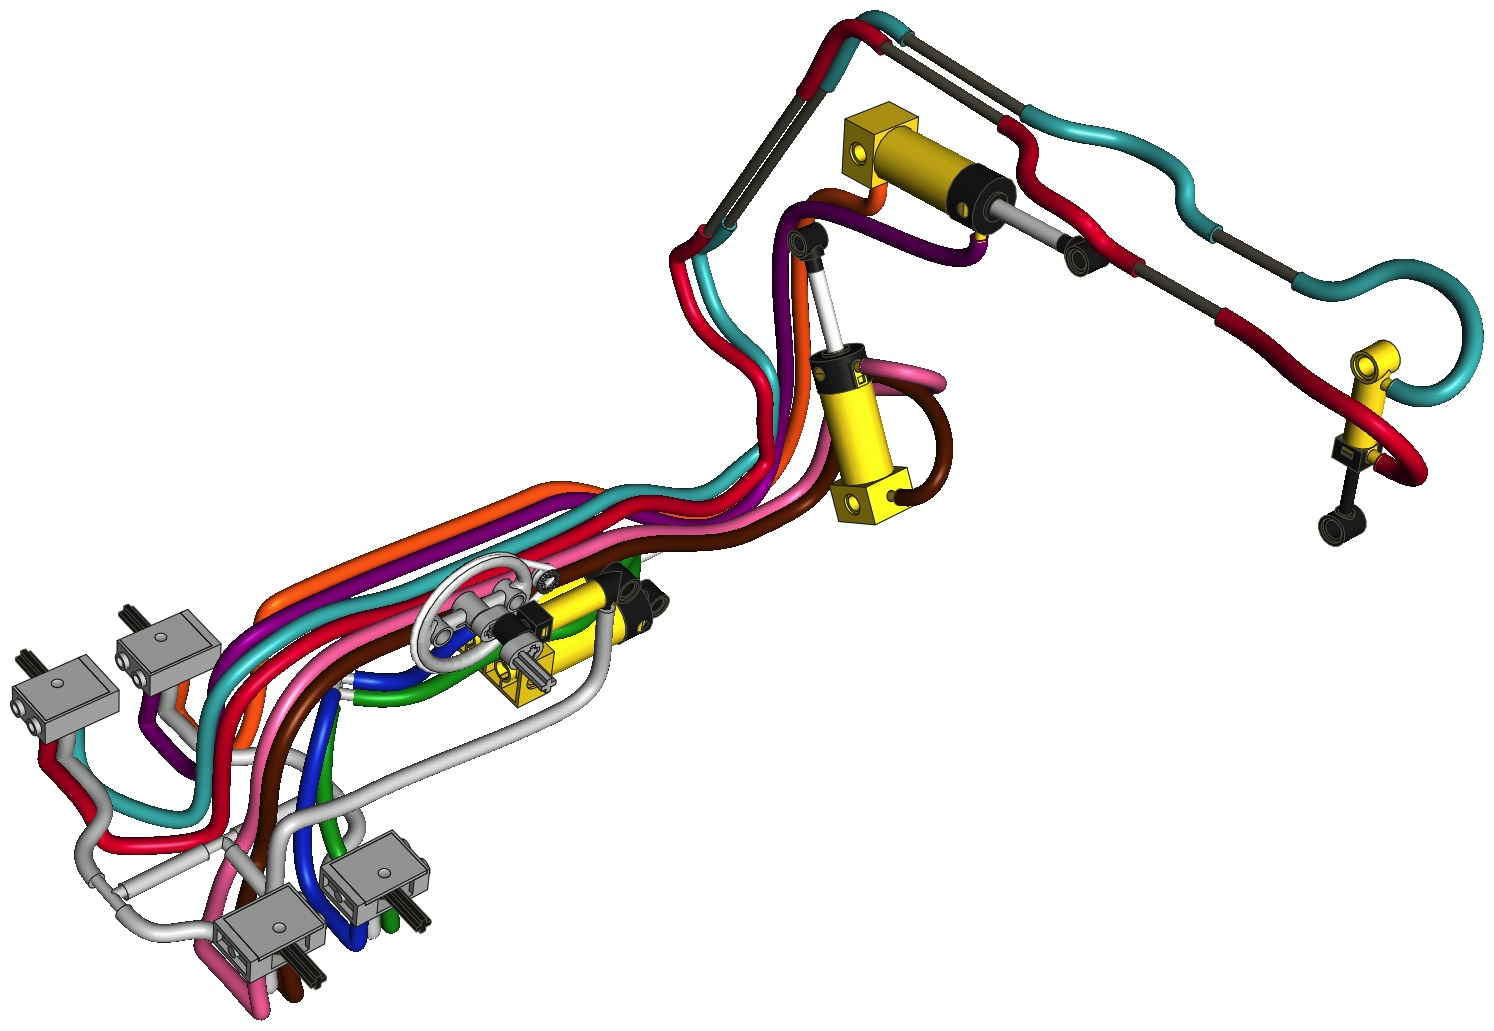
\includegraphics[width=0.99\textwidth]{1992_8868_truck_pneumatics_2.jpg}
\end{figure}
\end{frame}

\begin{frame}[fragile]{}
\begin{itemize}
\item[--] Makes use of revised pneumatics, which for the first time is powered by a motorised compressor  \vspace{3mm}
\item[--] The model is significantly more complex than anything so far, and instructions are still quite dense, involving only 32 steps. \vspace{3mm}
\item[--] A well crafted and realistic looking model with many sophisticated functions \vspace{3mm}
\end{itemize}
\end{frame}

\begin{frame}[fragile]{1994: 8880 Super car}
\begin{figure}[H]
 \centering
 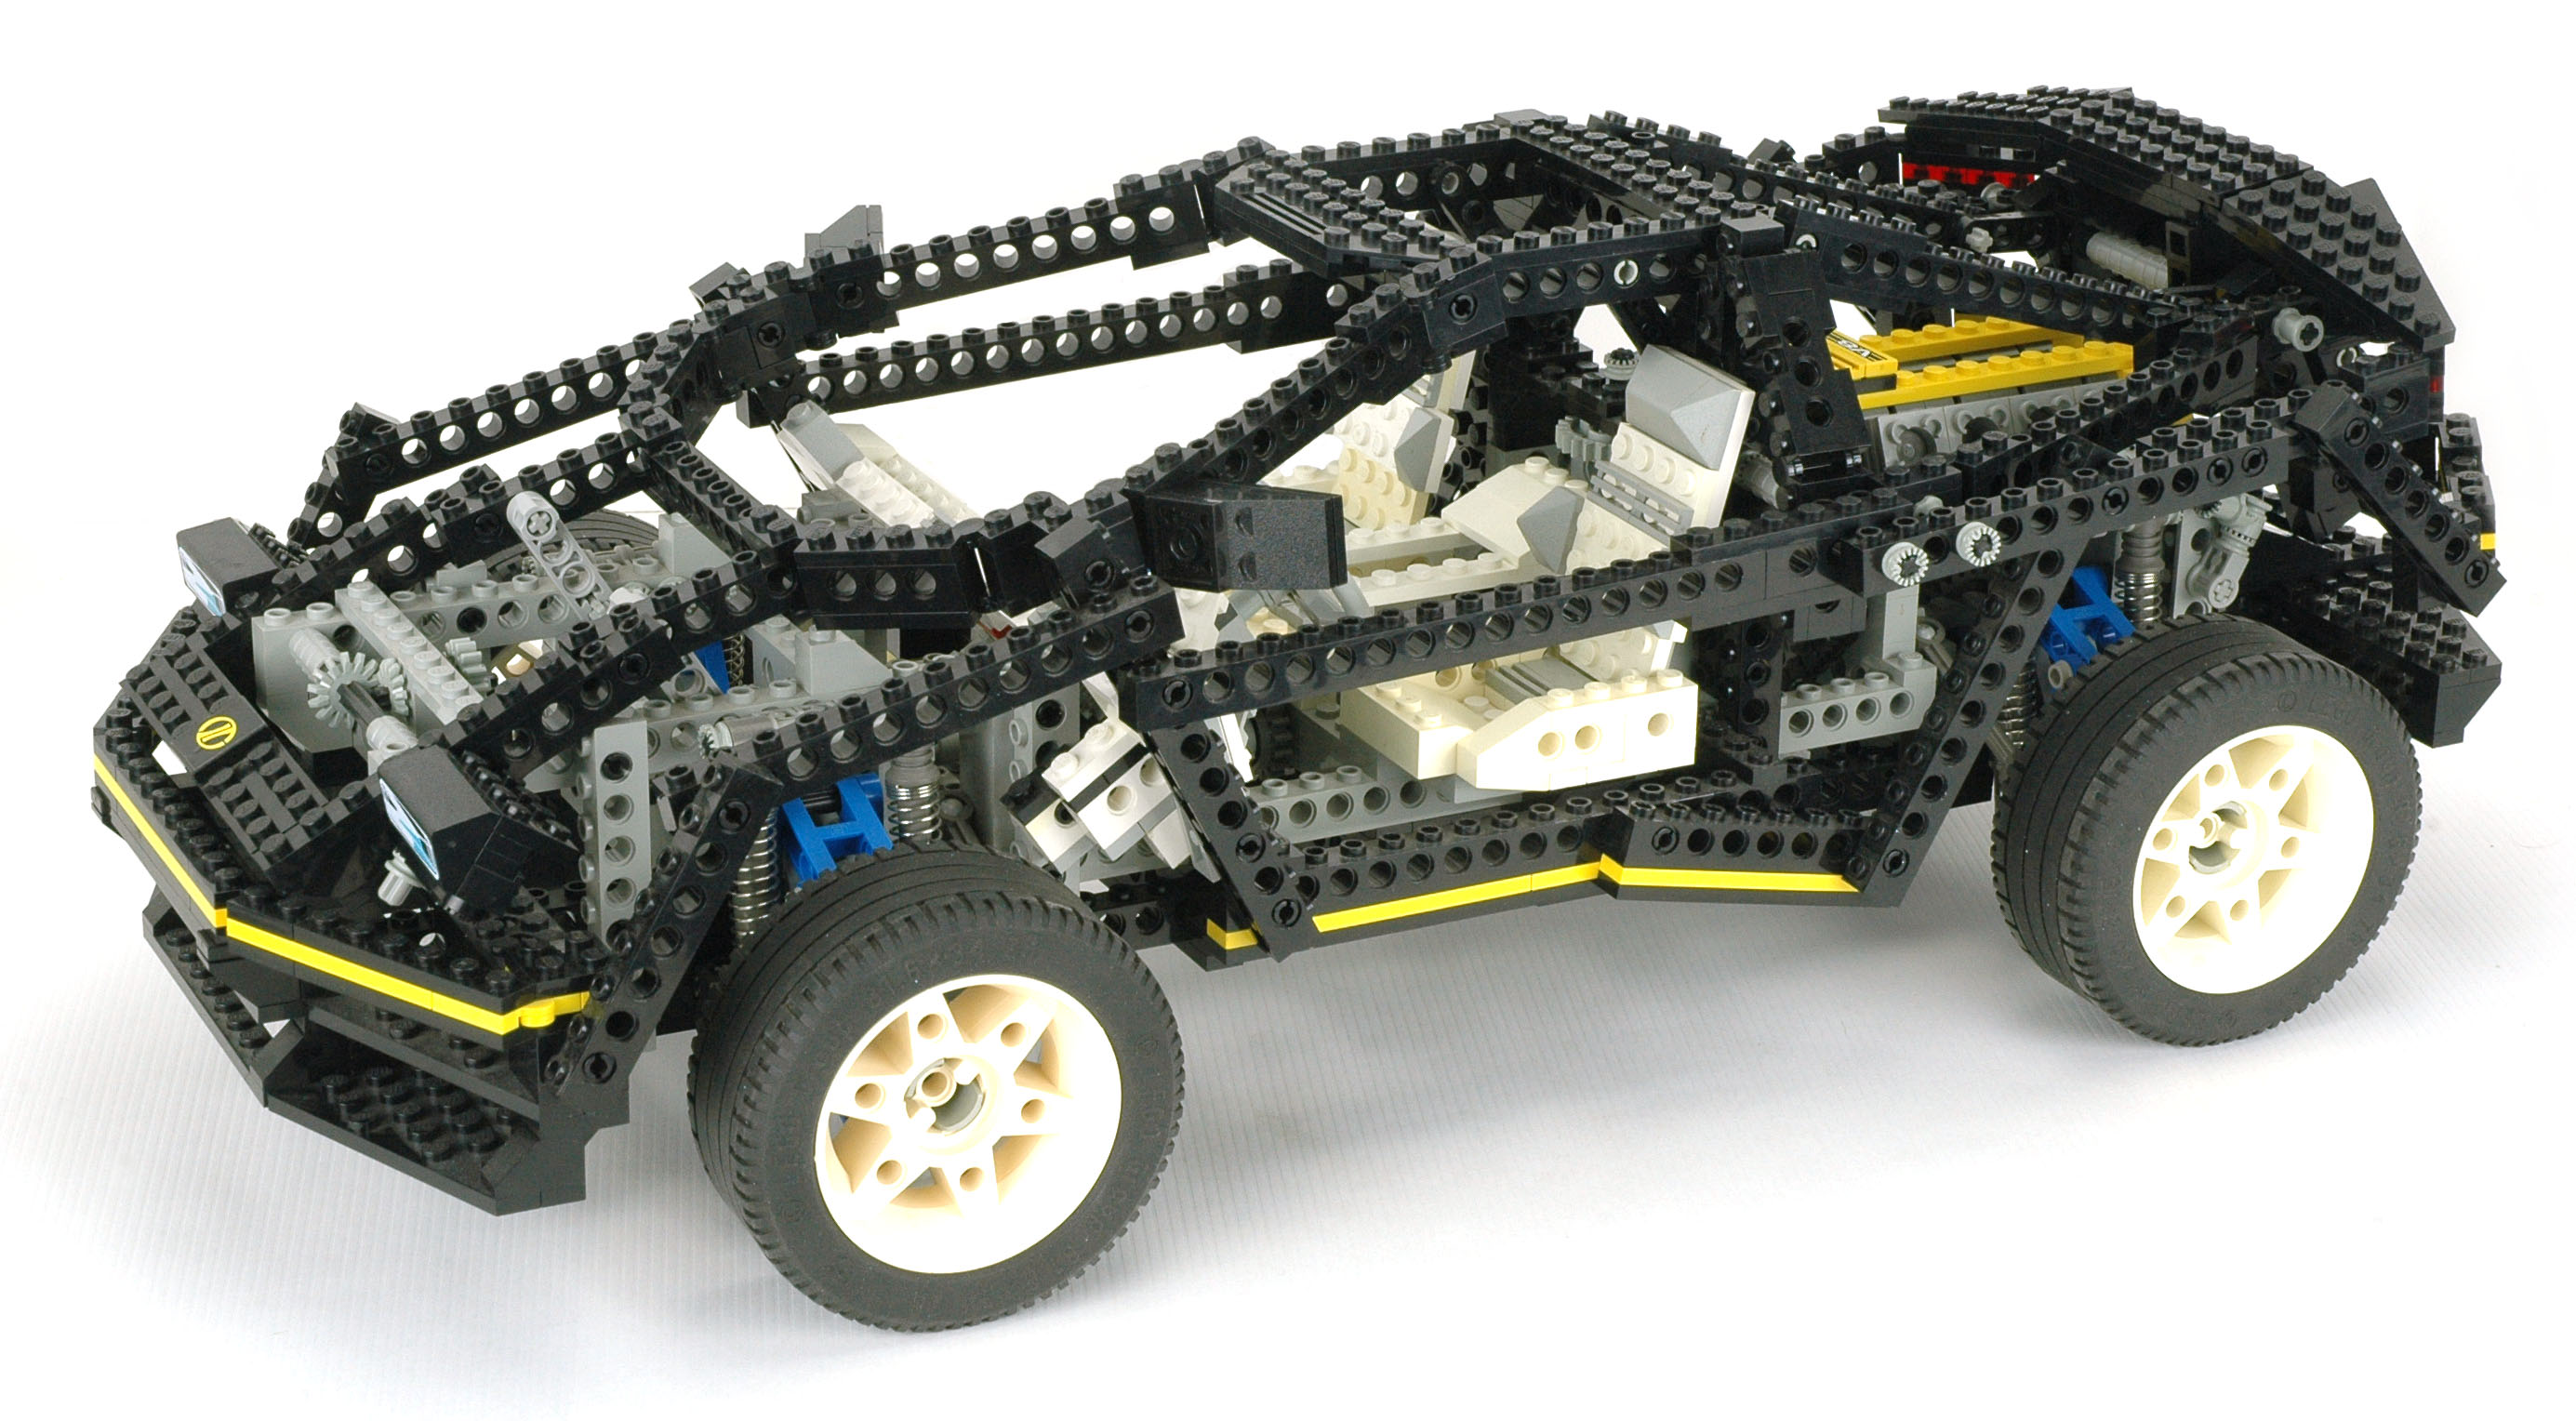
\includegraphics[width=0.99\textwidth]{1994_8880_car.jpg}
\end{figure}
\end{frame}

\begin{frame}[fragile]{Suspension}
\begin{figure}[H]
 \centering
 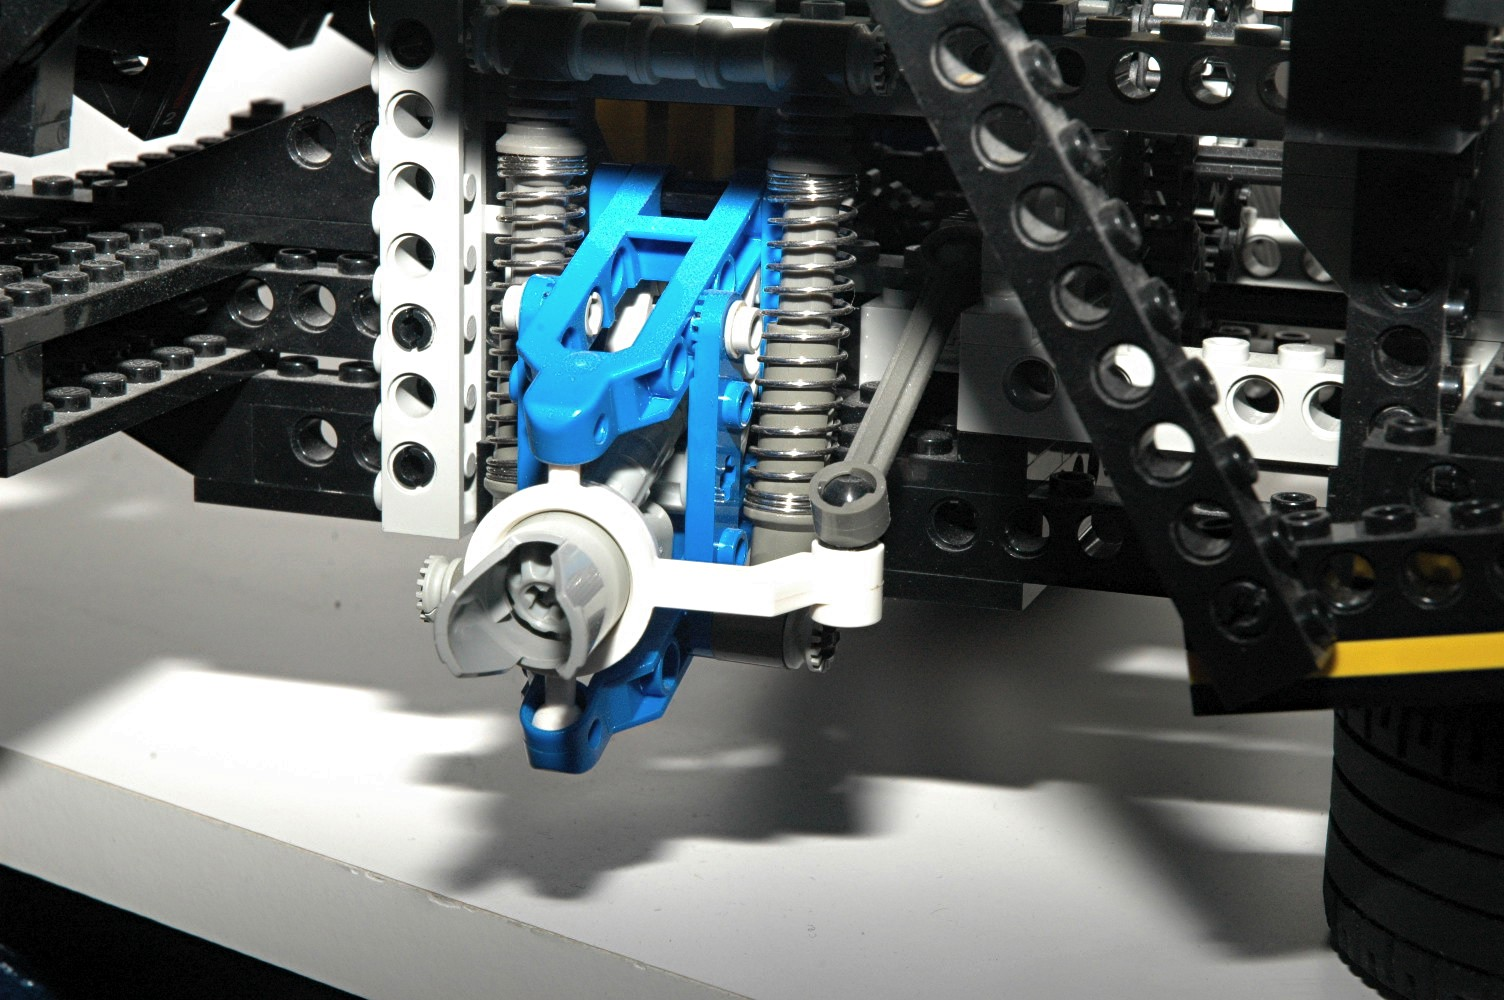
\includegraphics[width=0.9\textwidth]{1994_8880_car_suspension.jpg}
\end{figure}
\end{frame}

\begin{frame}[fragile]{Chassis}
\begin{figure}[H]
 \centering
 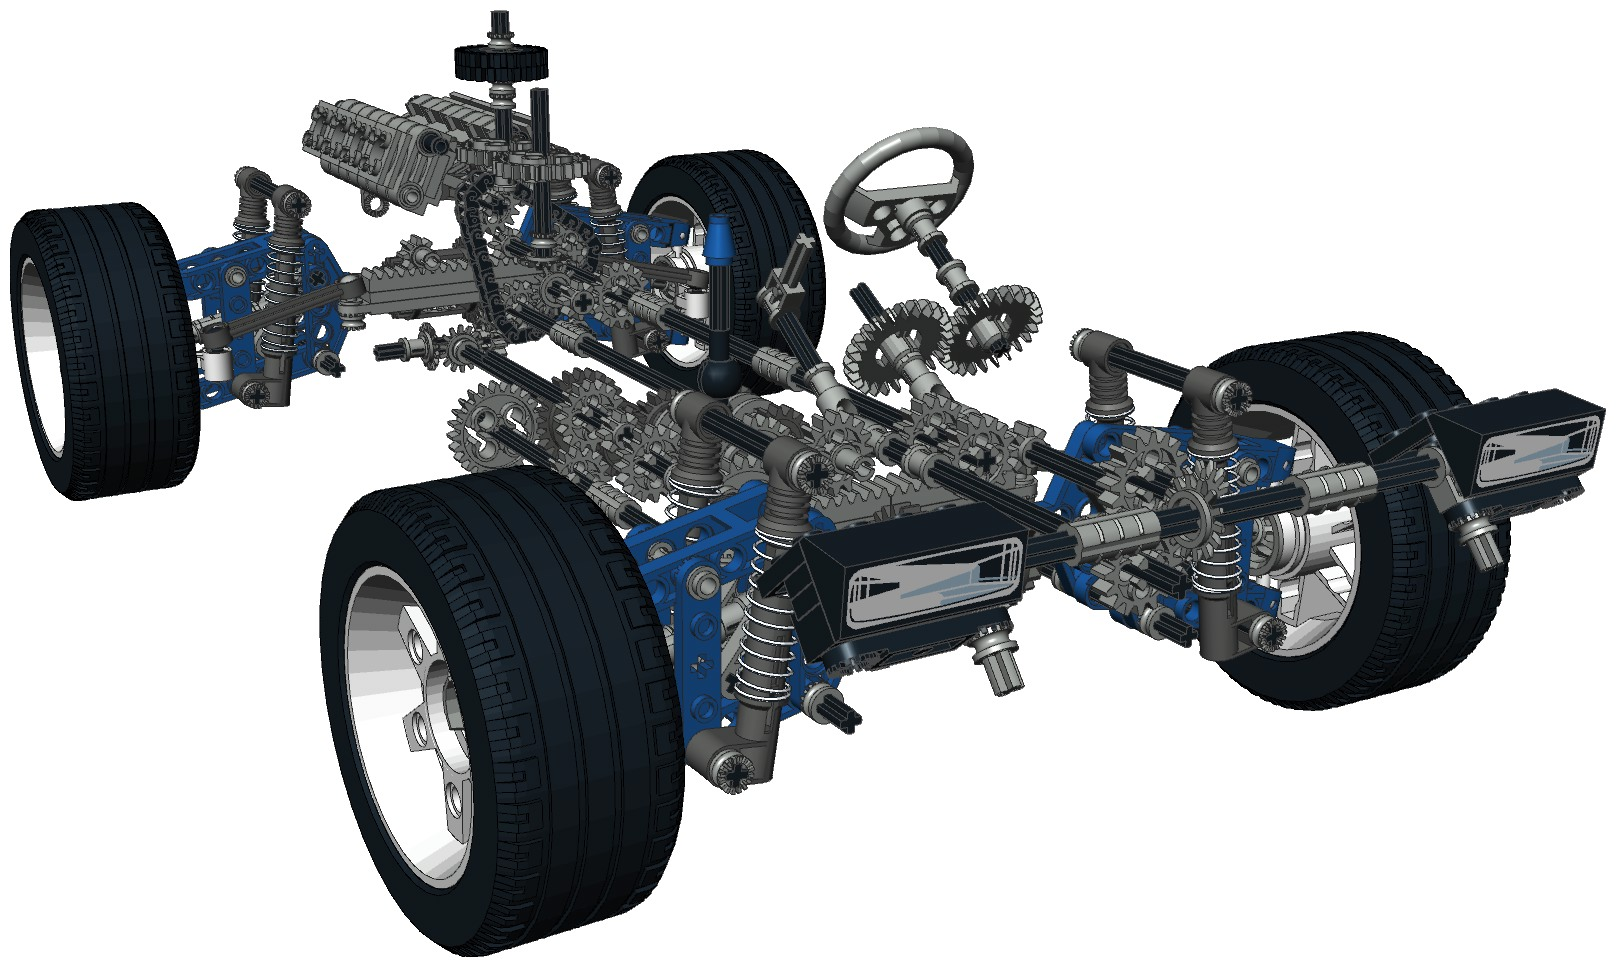
\includegraphics[width=0.99\textwidth]{1994_8880_car_chassis.jpg}
\end{figure}
\end{frame}

\begin{frame}[fragile]{}
\begin{itemize}
\item[--] This model represents the limits of what could be done with the existing Lego parts range.  \vspace{3mm}
\item[--] For the first time, the build of the model was too complicated to understand during the process of building \vspace{3mm}
\item[--] Steering, suspension and drive are all combined (and on all four wheels!) \vspace{3mm}
\end{itemize}
\end{frame}

\section{The game changer: ca. 1996 -- 2010}

\begin{frame}[fragile]{1996: Going studless}
\begin{figure}[H]
 \centering
 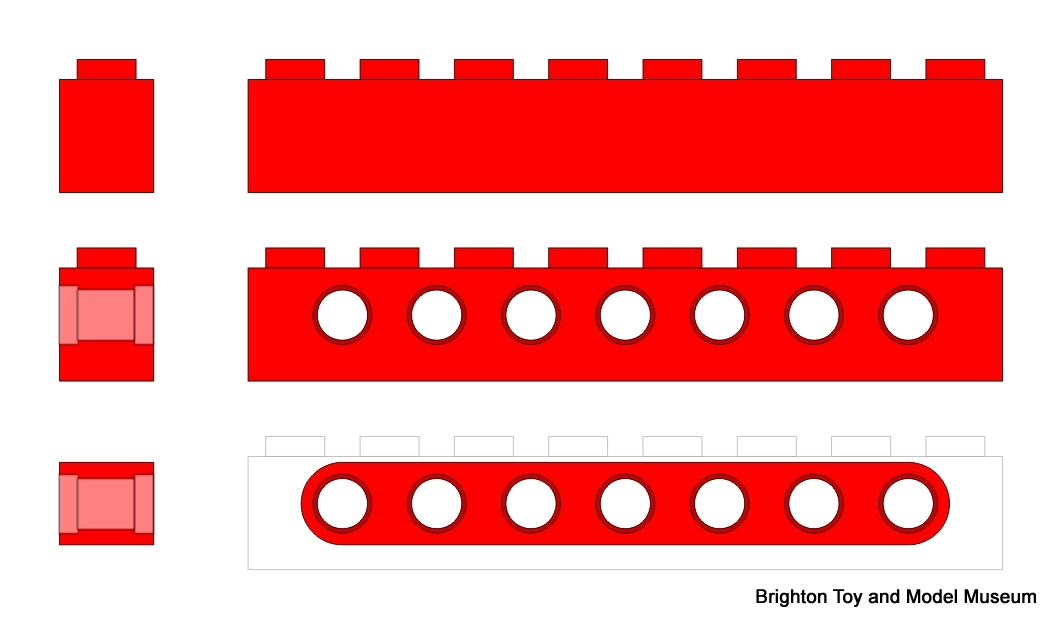
\includegraphics[width=0.99\textwidth]{1996_brick_studded_studless.jpg}
\end{figure}
\end{frame}

\begin{frame}[fragile]{1996: 8480 Shuttle}
\begin{figure}[H]
 \centering
 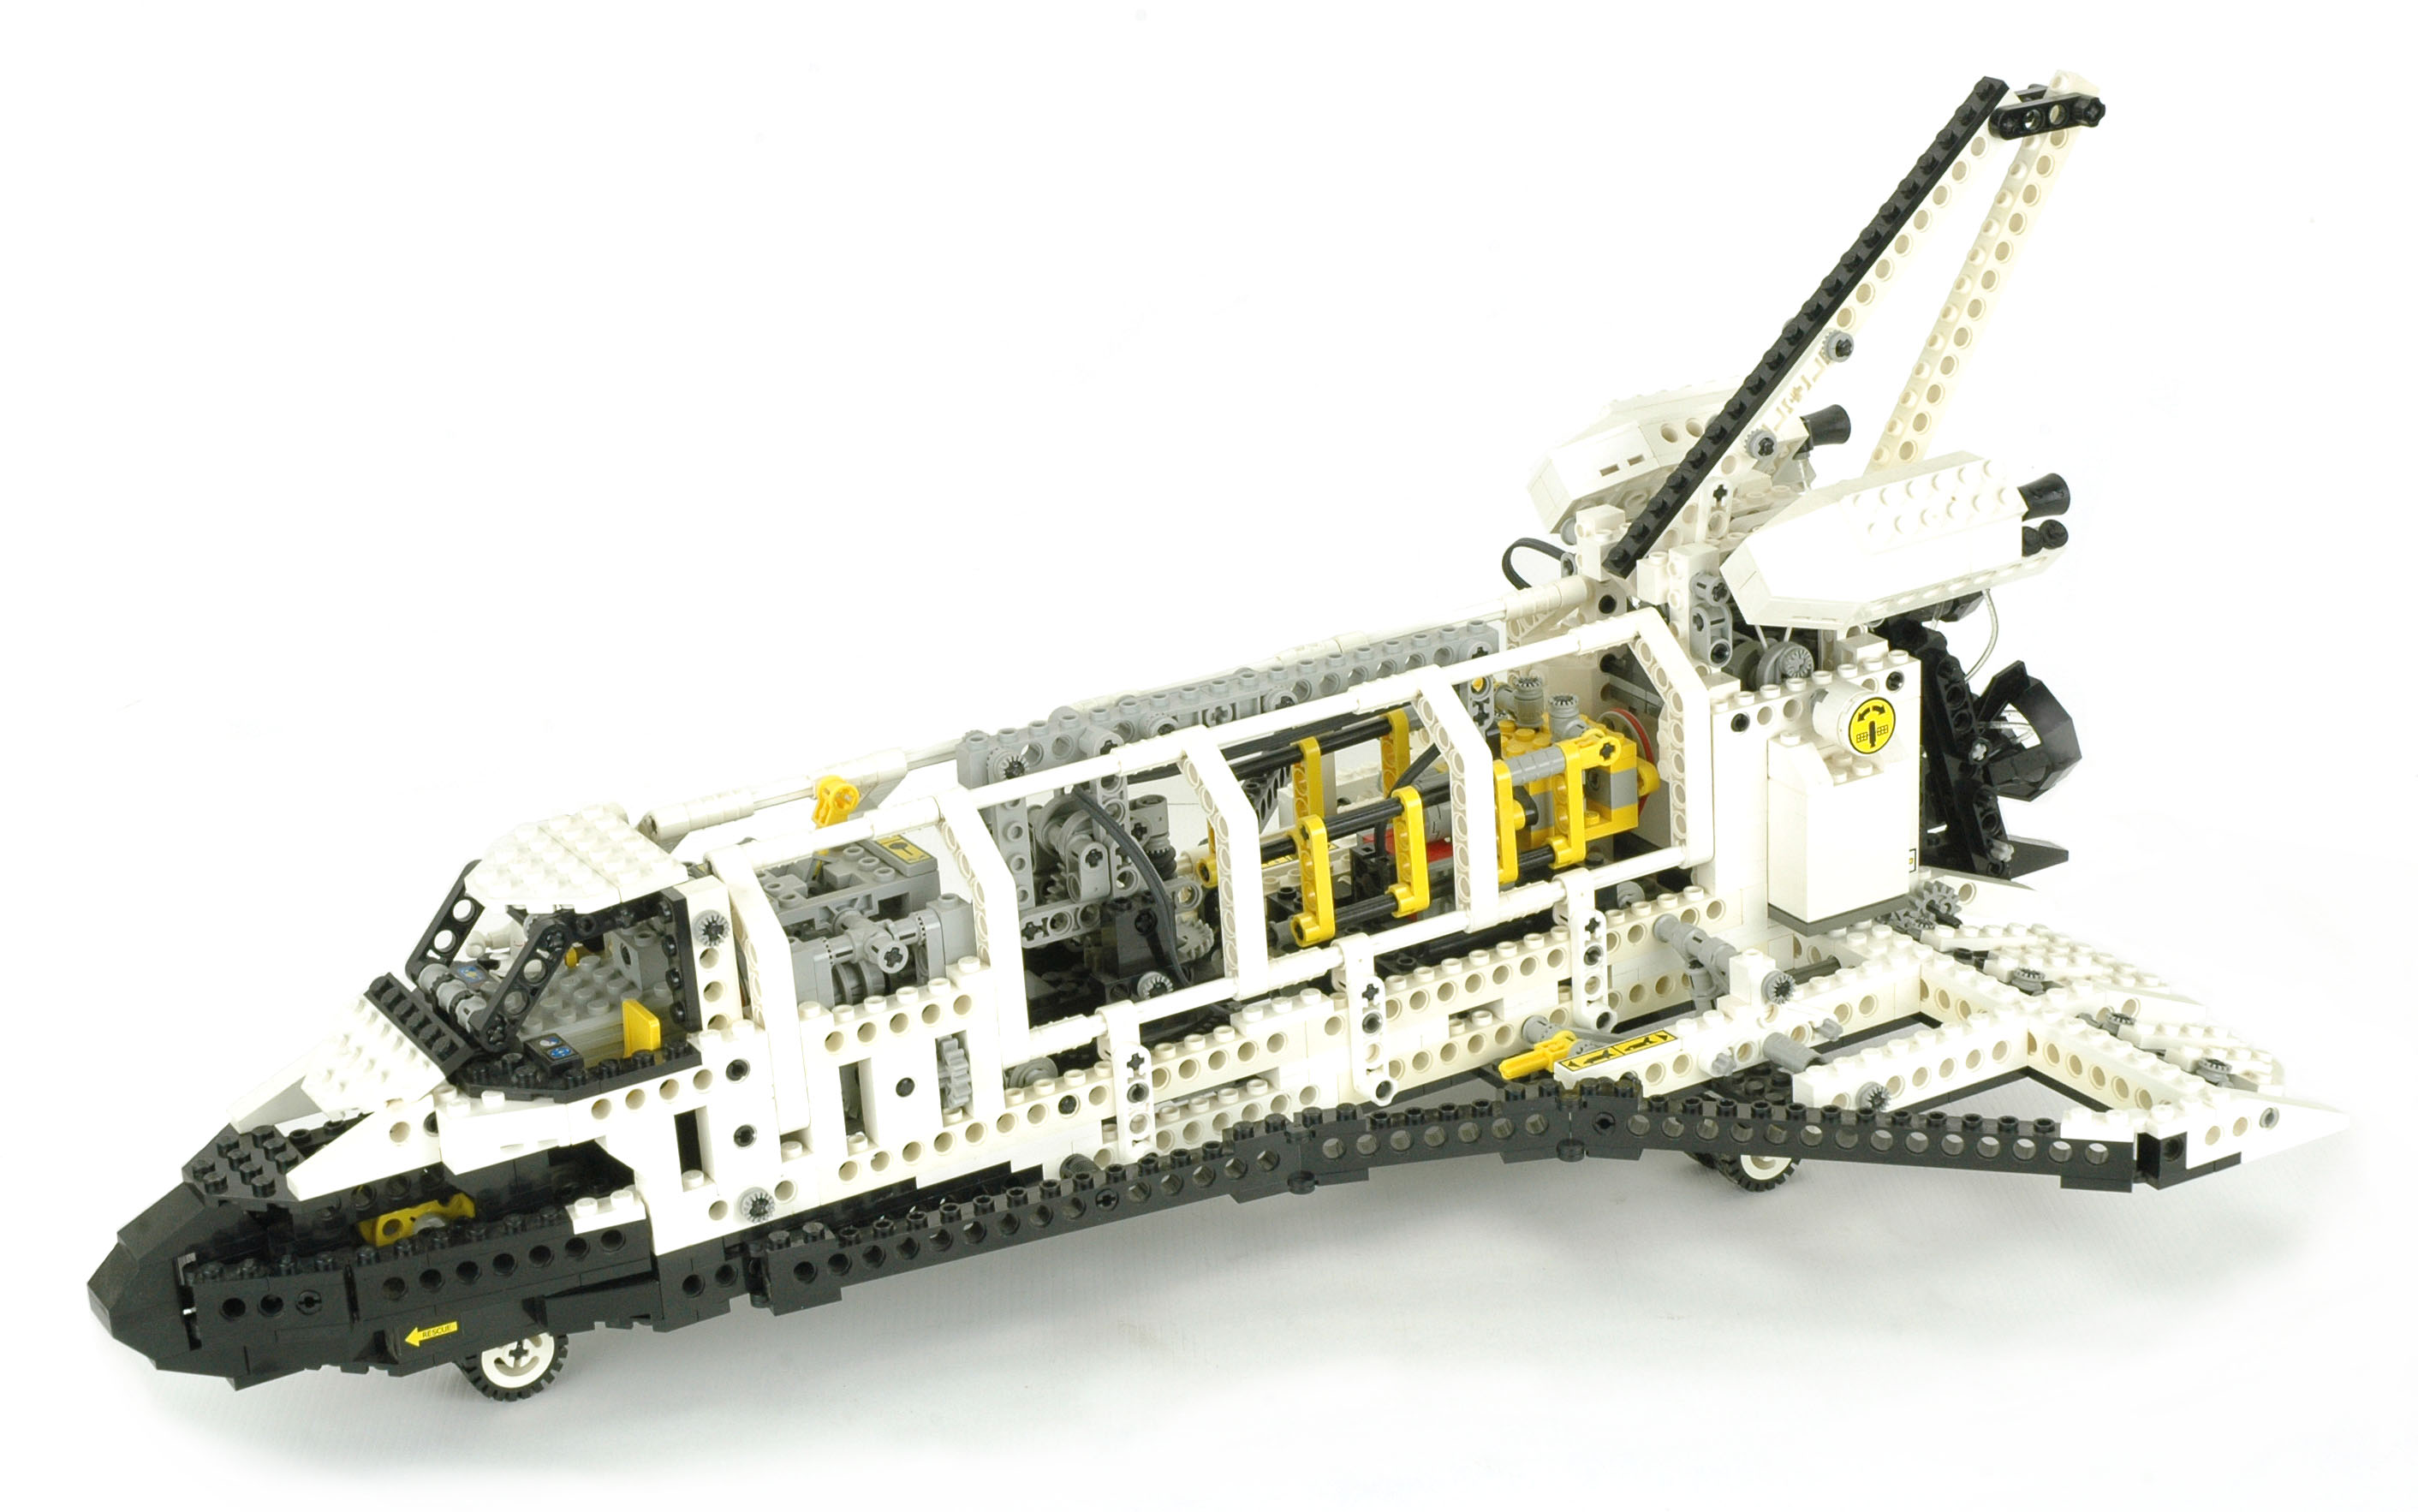
\includegraphics[width=0.99\textwidth]{1996_8480_shuttle.jpg}
\end{figure}
\end{frame}

\begin{frame}[fragile]{}
\begin{itemize}
\item[--] The transition from studded beam construction to studless took a long time. Early use was superficial, mainly for styling. \vspace{3mm}
\item[--] Building studlessly required a very different approach: building from inside out, rather than bottom to top. \vspace{3mm}
\item[--] This small change was a stroke of genius: it kept backward compatibility whilst facilitating angular beams \vspace{3mm}
\end{itemize}
\end{frame}

\begin{frame}[fragile]{\sout{Backward} compatibility elsewhere...}
\begin{figure}[H]
 \centering
 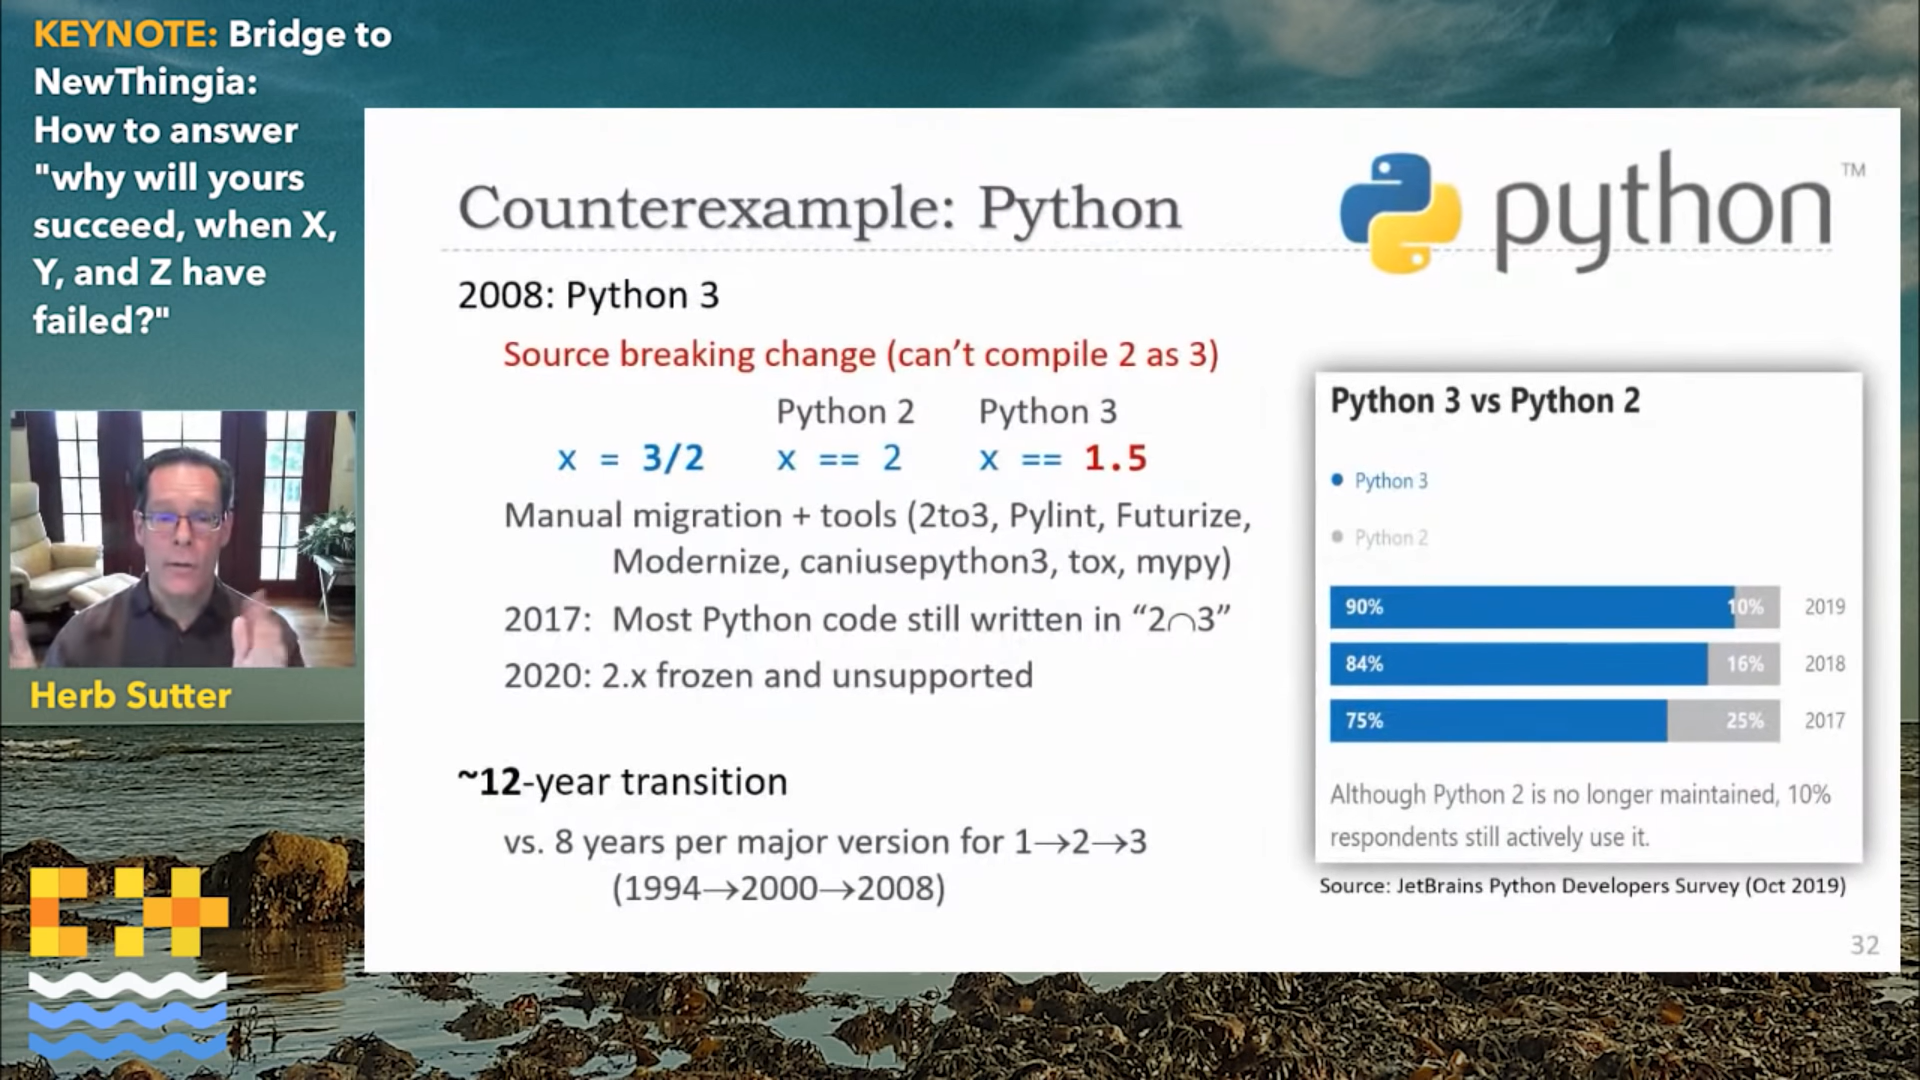
\includegraphics[width=0.99\textwidth]{python_backward_compatibility.png}
\end{figure}
\end{frame}

\begin{frame}[fragile]{Breaking change costs 10 years}
\begin{figure}[H]
 \centering
 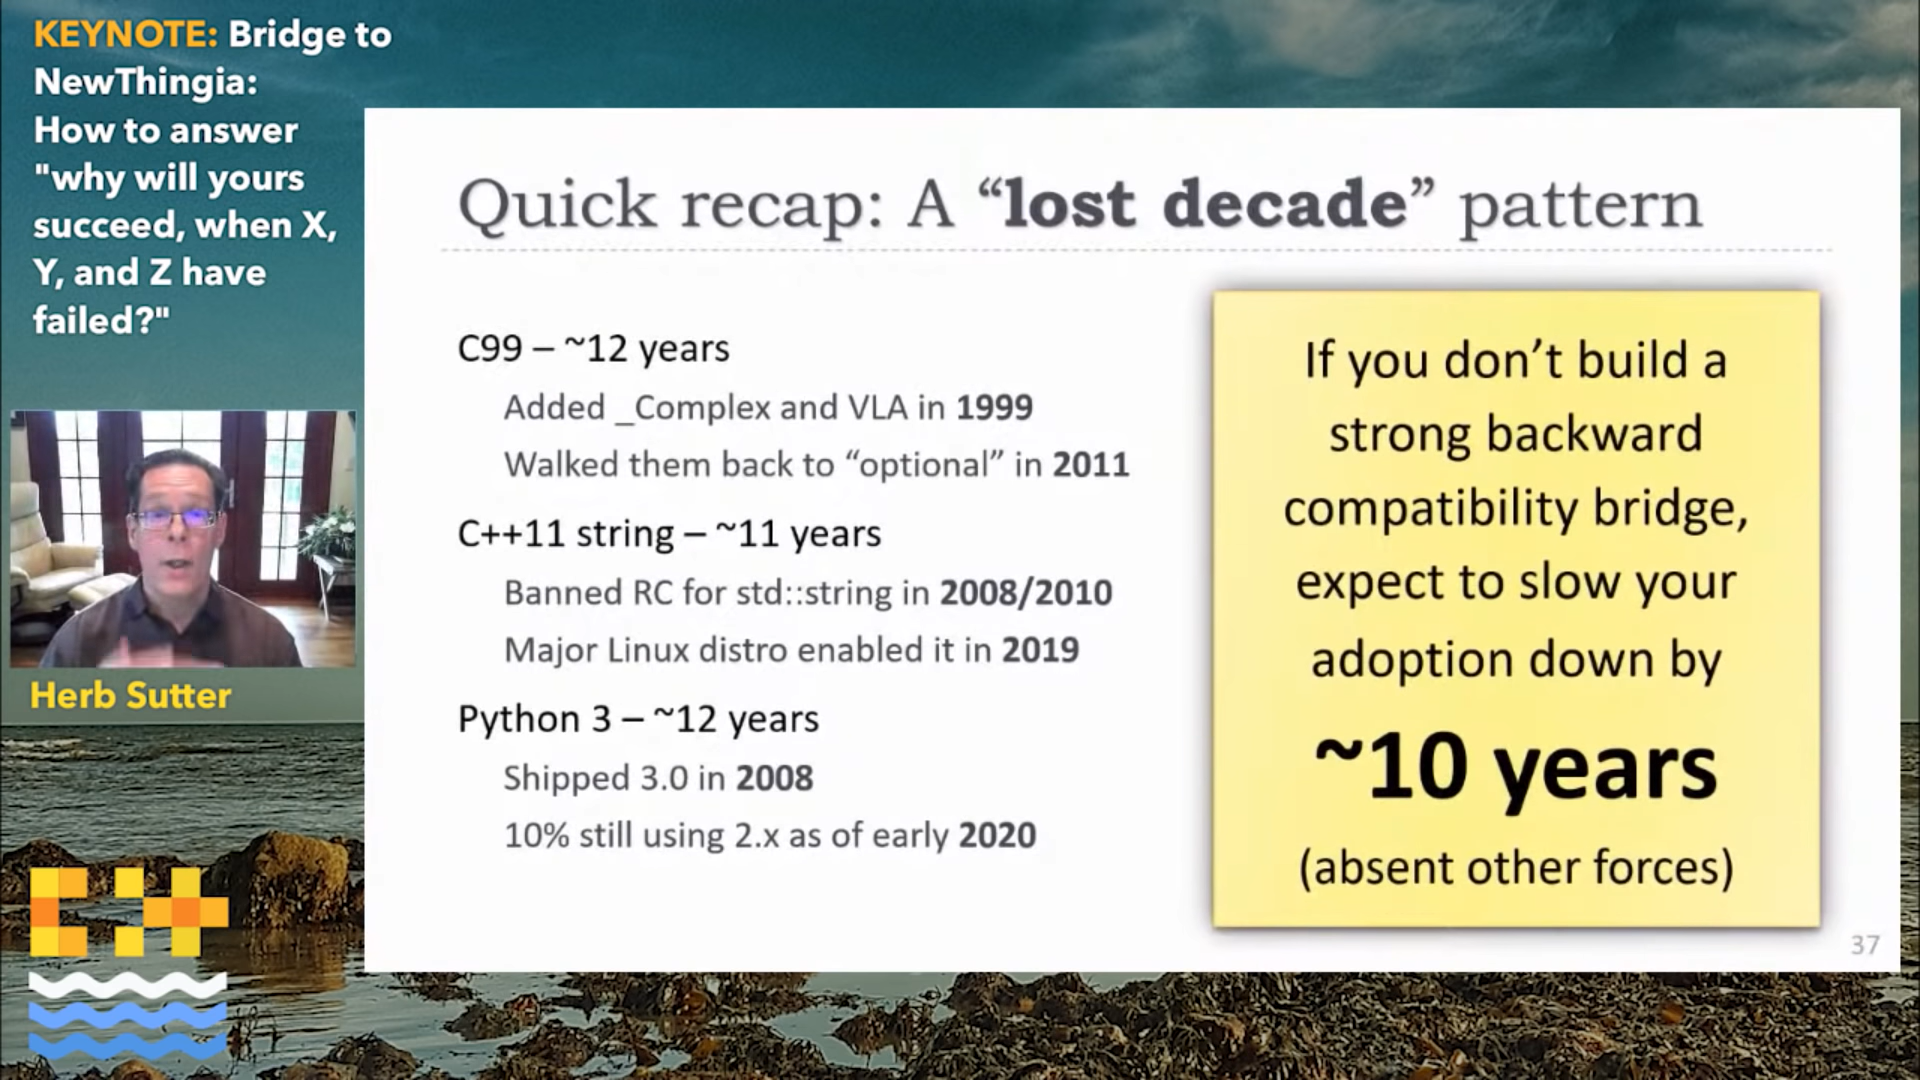
\includegraphics[width=0.99\textwidth]{backward_compatibility.png}
\end{figure}
\end{frame}


\section{Lost in toydom: ca. 1998 -- 2001}

\begin{frame}[fragile]{1998: 8462}
\begin{figure}[H]
 \centering
 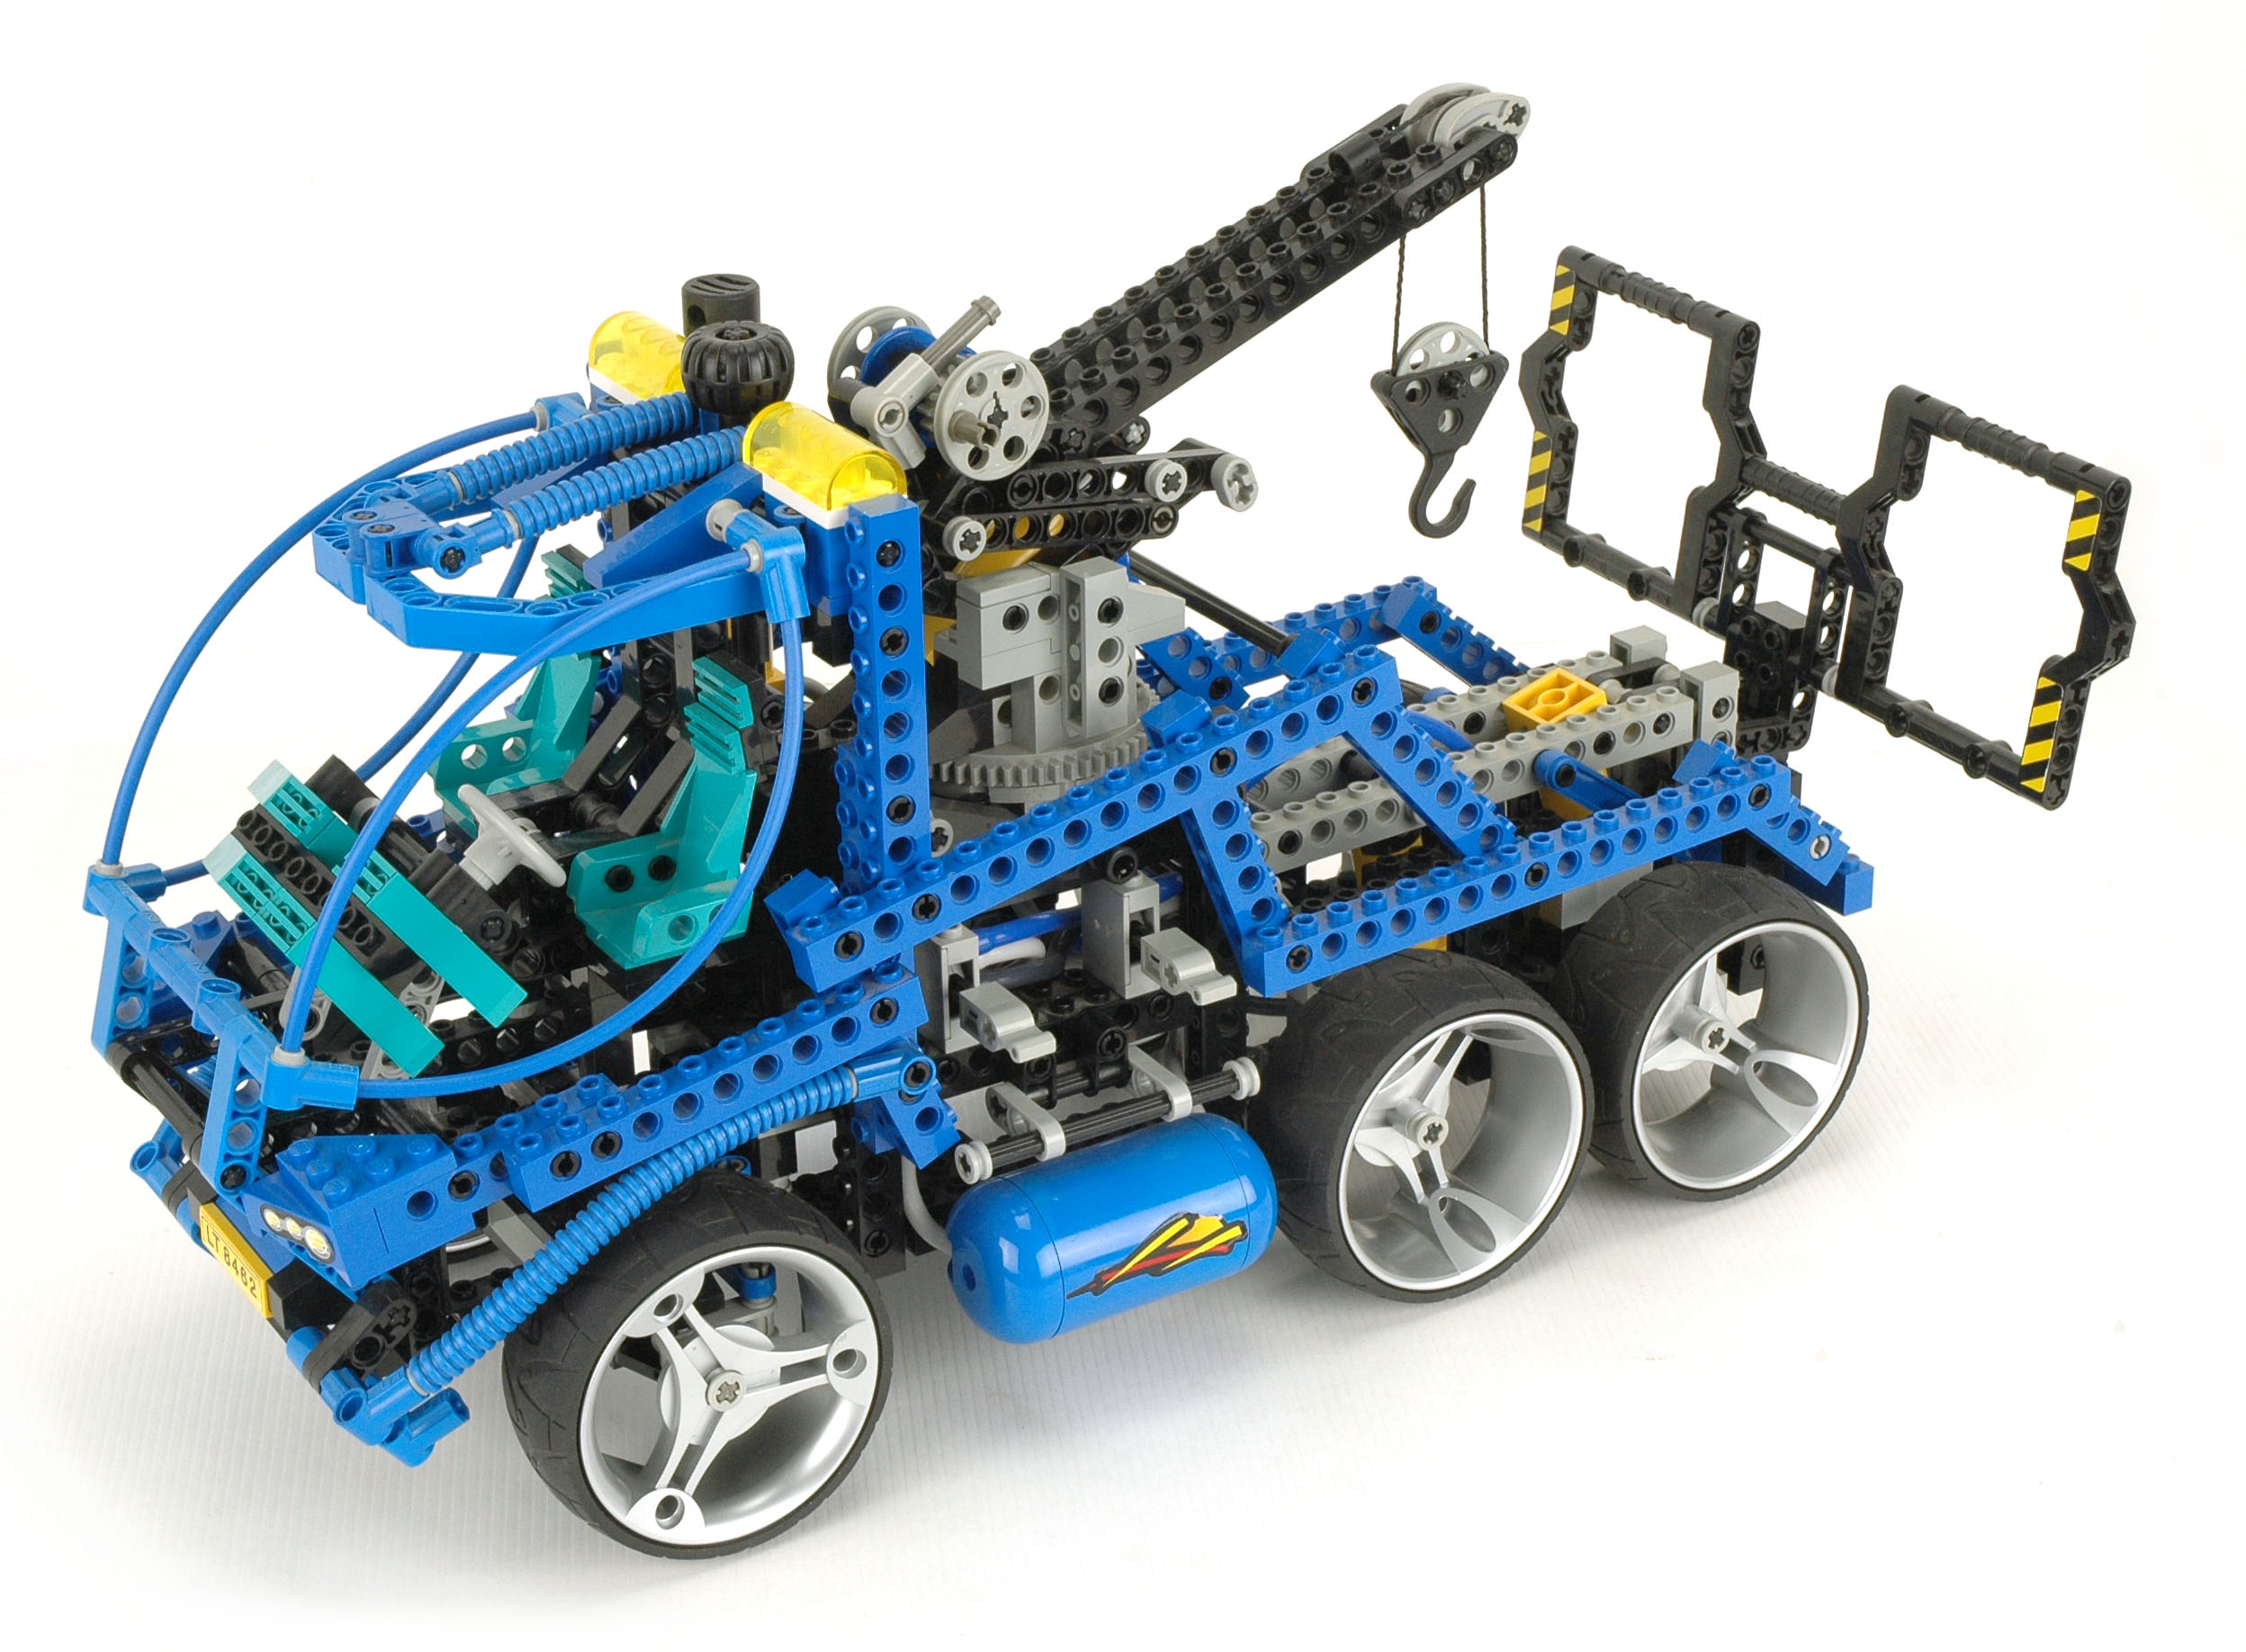
\includegraphics[width=0.99\textwidth]{1998_8462_truck.jpg}
\end{figure}
\end{frame}

\begin{frame}[fragile]{1999: 8448}
\begin{figure}[H]
 \centering
 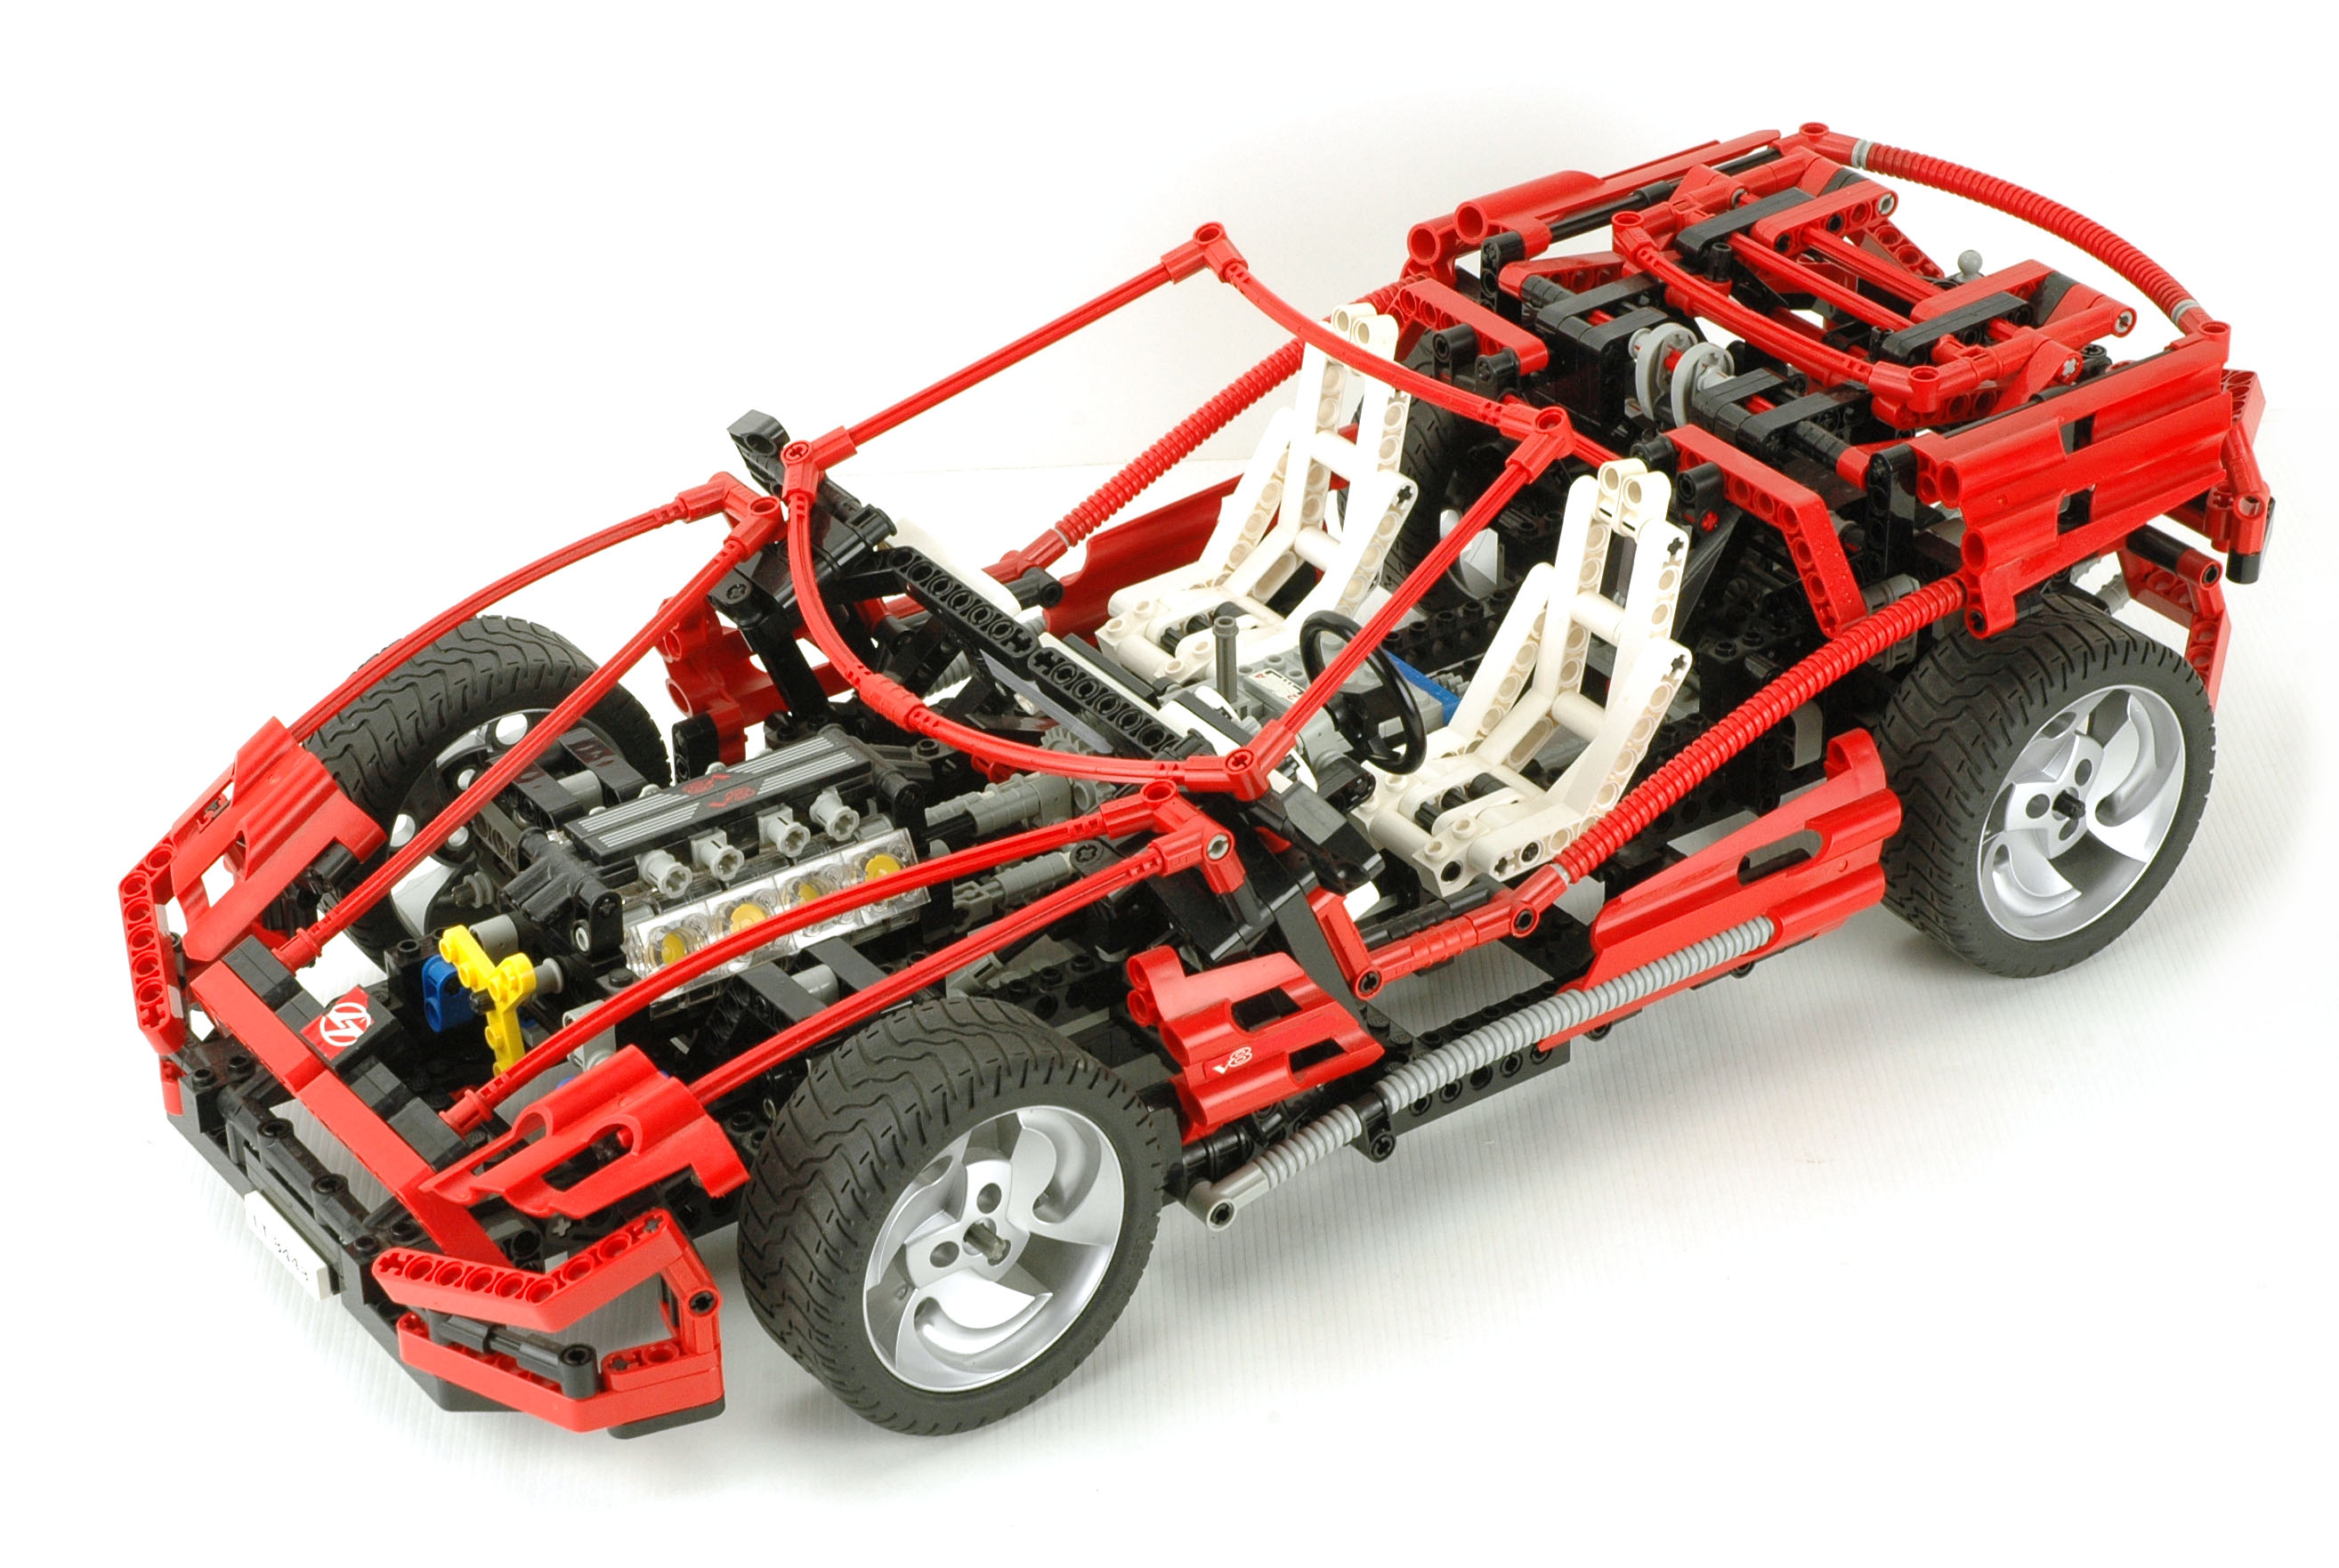
\includegraphics[width=0.99\textwidth]{1999_8448_car.jpg}
\end{figure}
\end{frame}

\begin{frame}[fragile]{2001: 8466}
\begin{figure}[H]
 \centering
 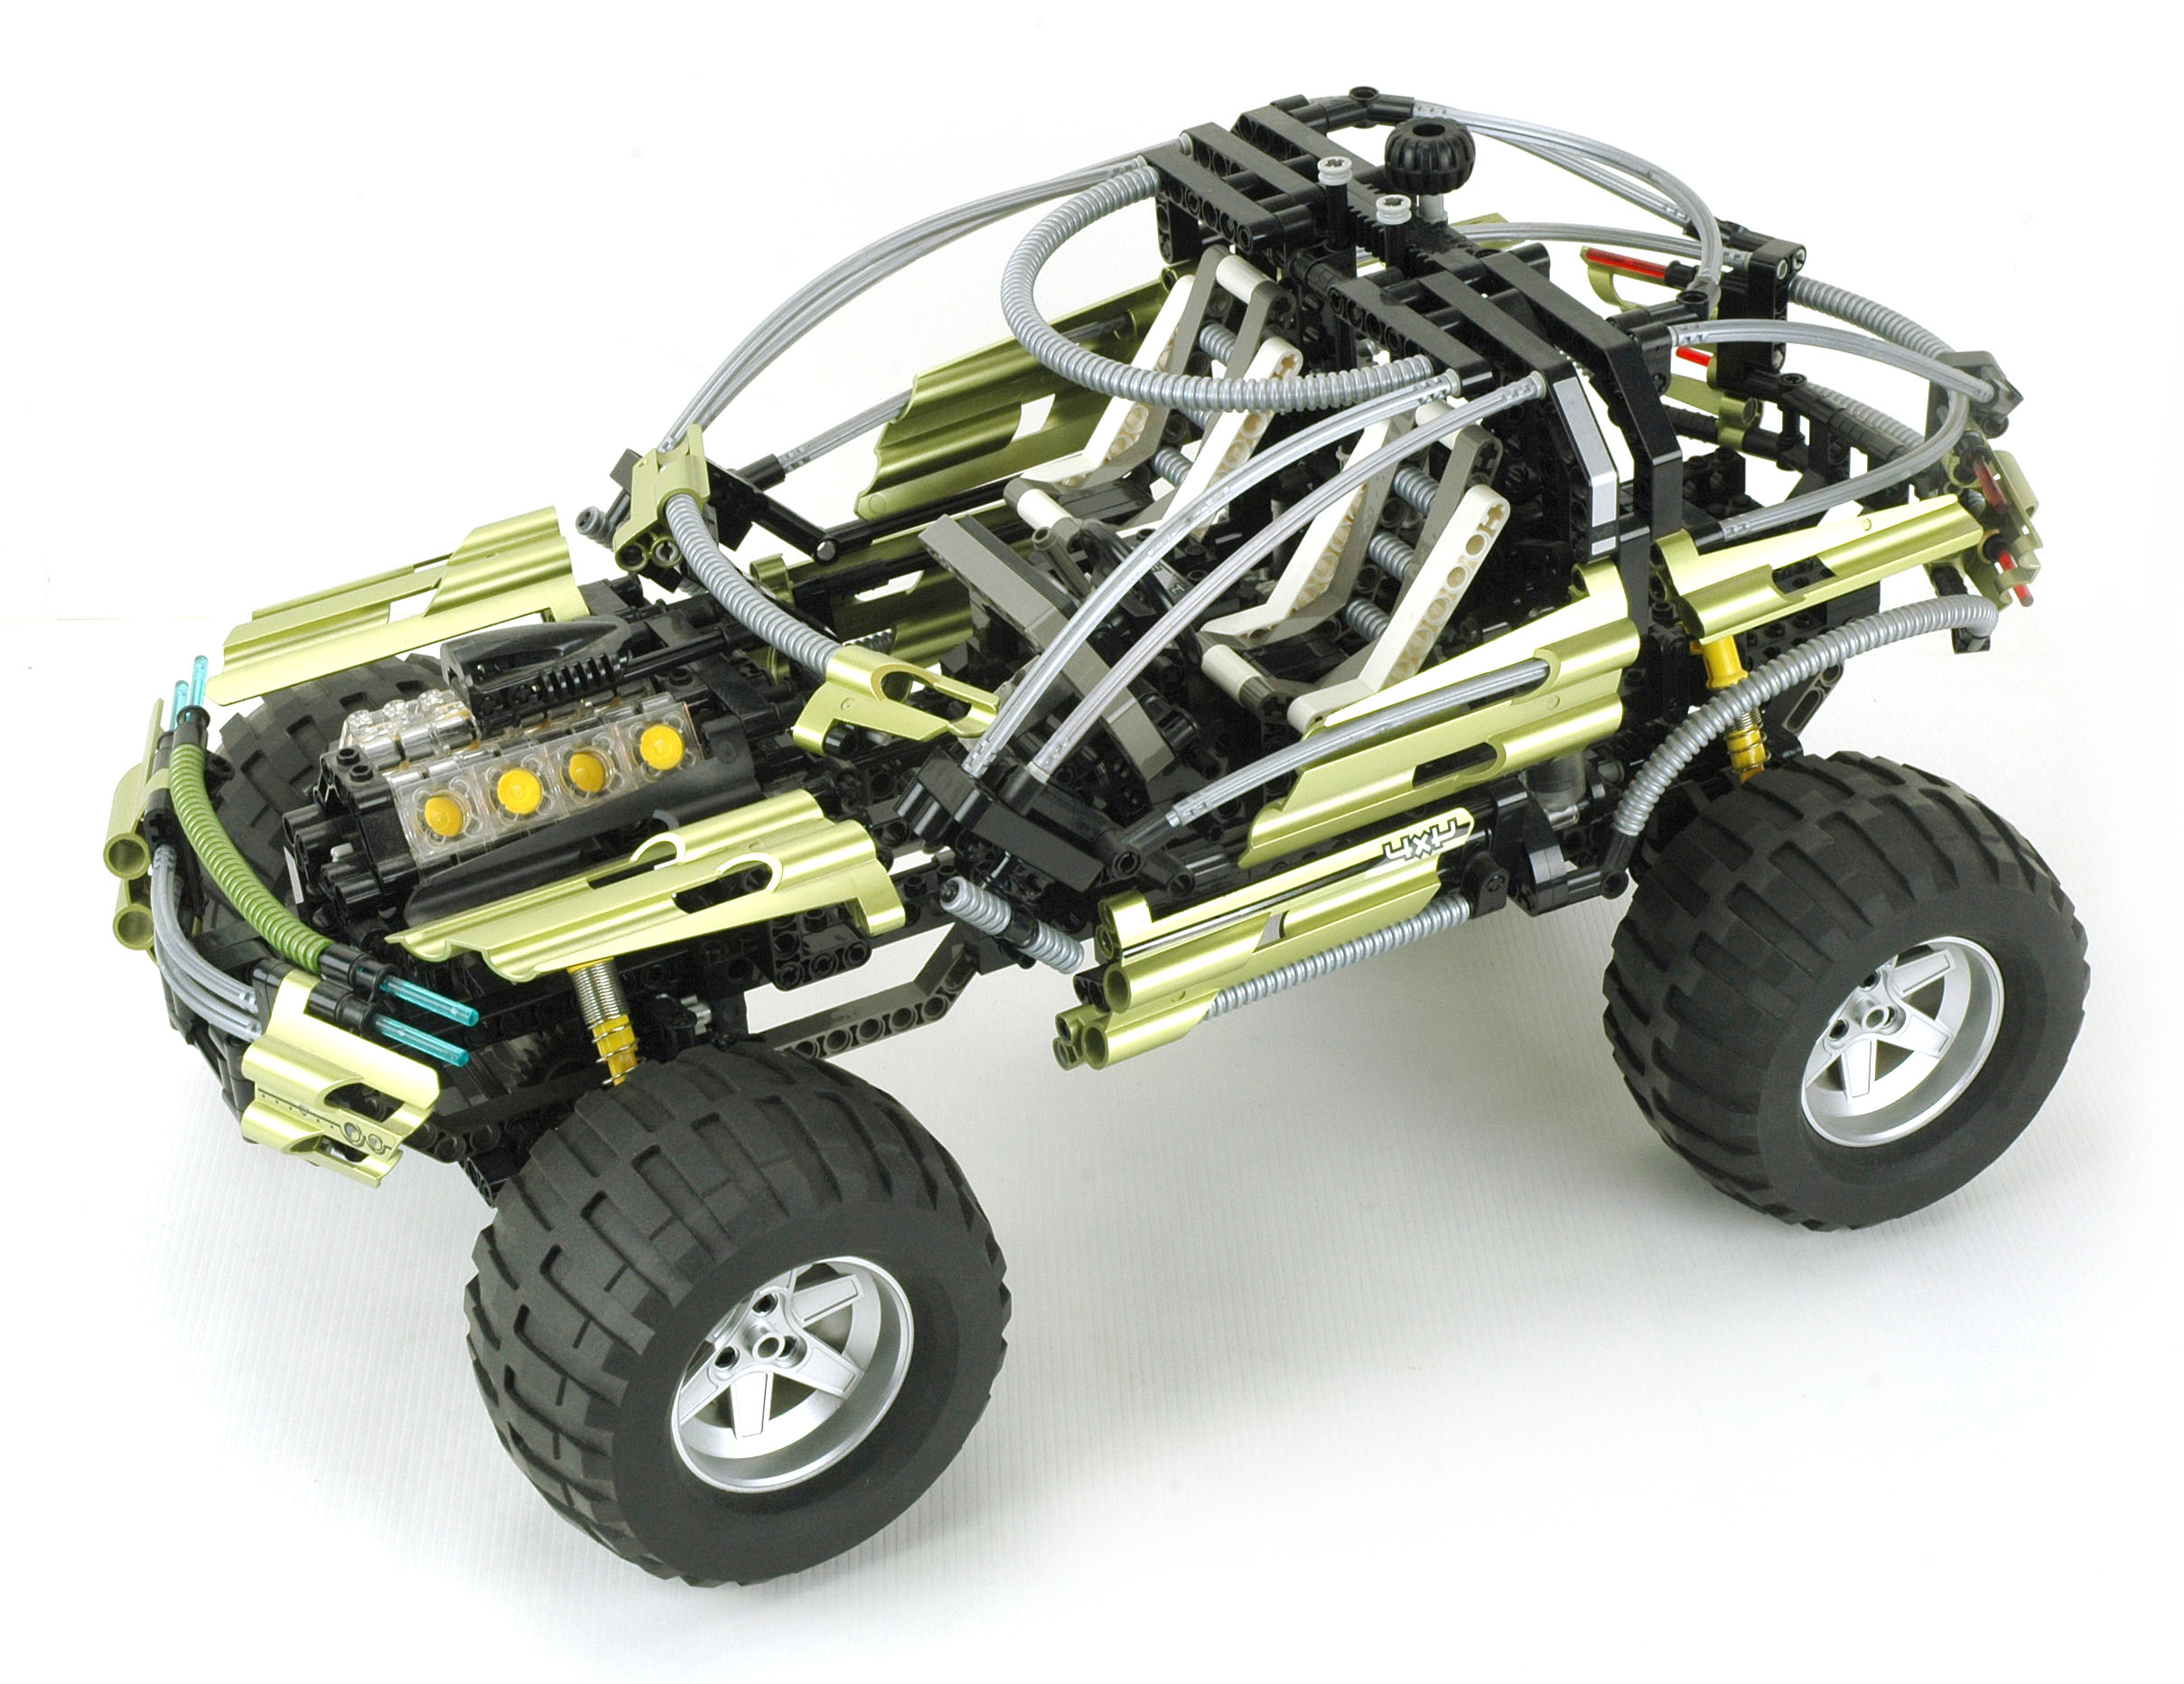
\includegraphics[width=0.9\textwidth]{2001_8466_truck.jpg}
\end{figure}
\end{frame}

\begin{frame}[fragile]{}
\begin{itemize}
\item[--] For some reason, coincidentally with the introduction of studless beams, models took a turn for the worse, attempting to appeal to the kool kids  \vspace{3mm}
\item[--] This was a grave error of judgement. Lego Technic was never cool (but is was acceptable) \vspace{3mm}
\item[--] There seemed to be wider trends throughout Lego, seeming to lose sight of its roots. Consequently, the business almost went bust \vspace{3mm}
\end{itemize}
\end{frame}

\begin{frame}[fragile]{2003 financial crisis}
\begin{figure}[H]
 \centering
 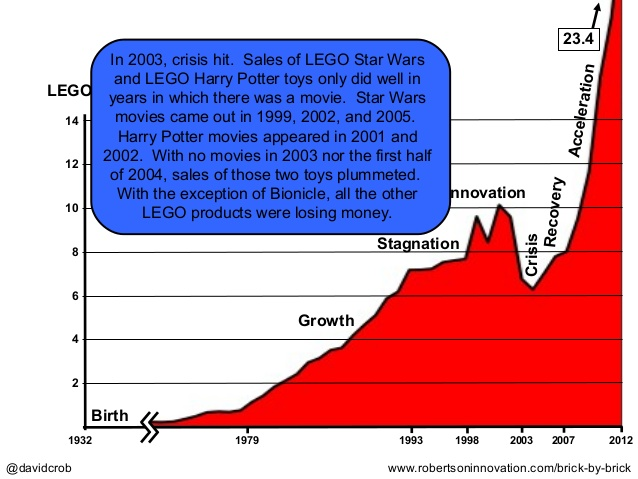
\includegraphics[width=0.9\textwidth]{2003_lego_sales_2003.jpg}
\end{figure}
\end{frame}

\section{I'm not a toy: ca. 2003 -- present}

\begin{frame}[fragile]{2005: 8421 Mobile crane (1884 pc.)}
\begin{figure}[H]
 \centering
 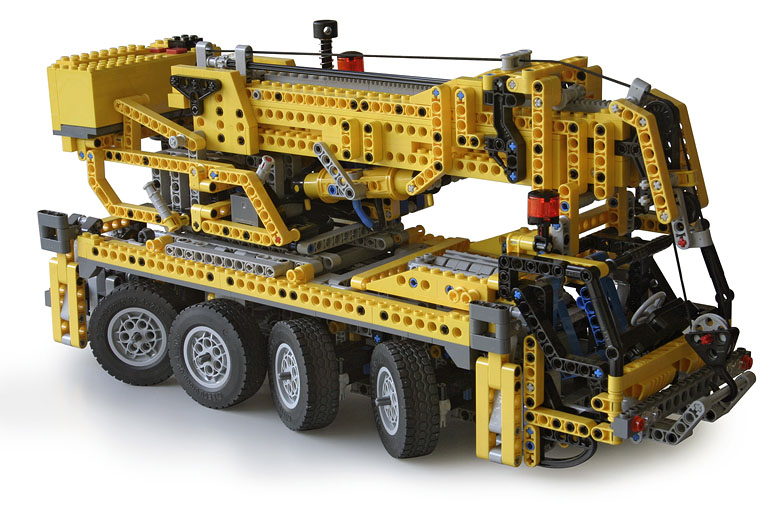
\includegraphics[width=0.99\textwidth]{2005_8421_crane.jpg}
\end{figure}
\end{frame}

\begin{frame}[fragile]{2007: 8275 Bulldozer (1405 pc.)}
\begin{figure}[H]
 \centering
 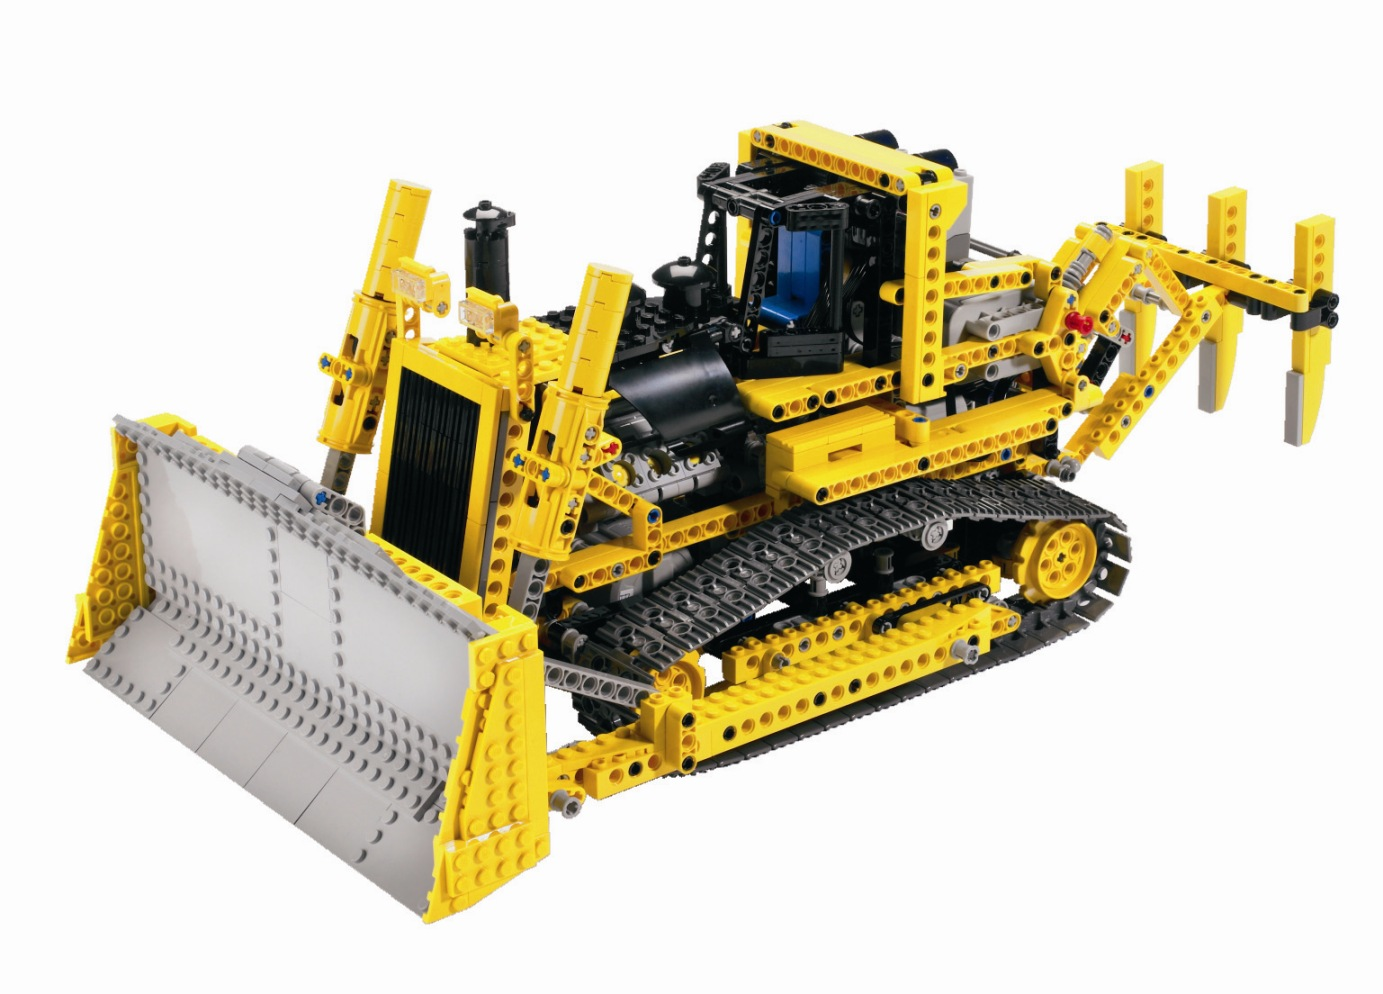
\includegraphics[width=0.99\textwidth]{2007_8275_bulldozer.jpg}
\end{figure}
\end{frame}

\begin{frame}[fragile]{2010: 8043 Excavator (1127 pc.)}
\begin{figure}[H]
 \centering
 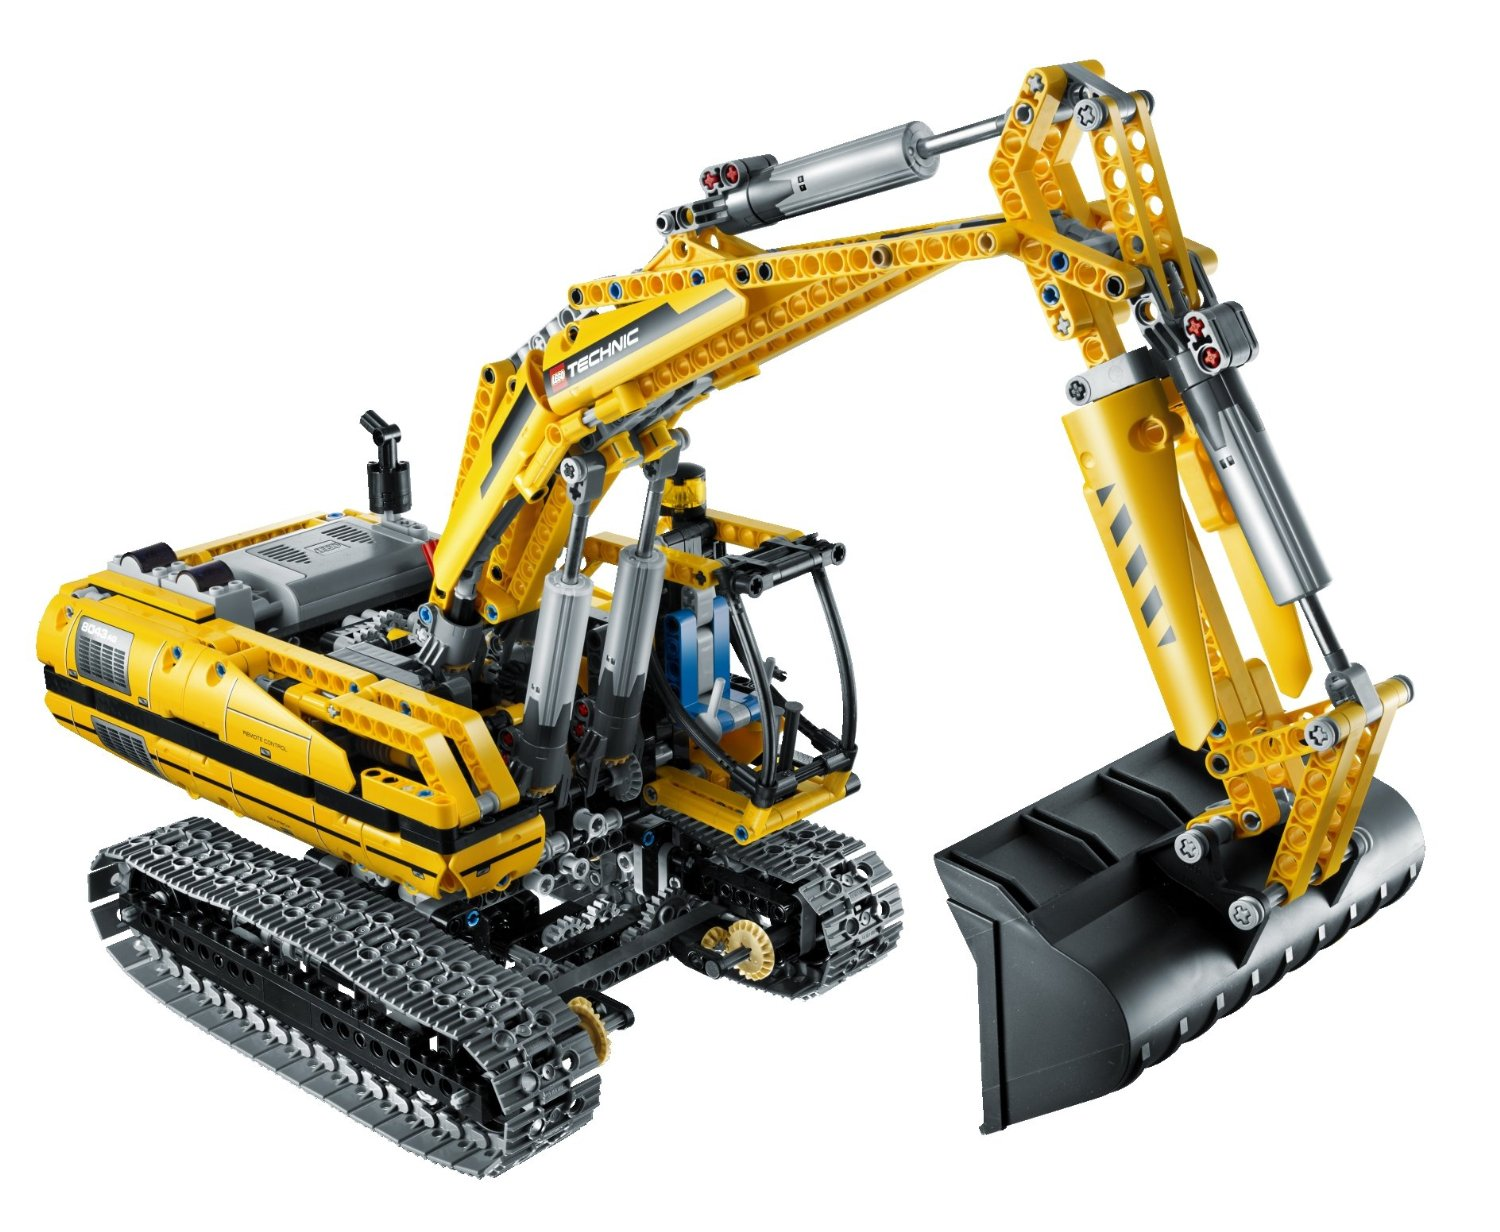
\includegraphics[width=0.88\textwidth]{2010_8043_excavator.jpg}
\end{figure}
\end{frame}

\begin{frame}[fragile]{2015: 42043 Mercedes-Benz Arocs}
\begin{figure}[H]
 \centering
 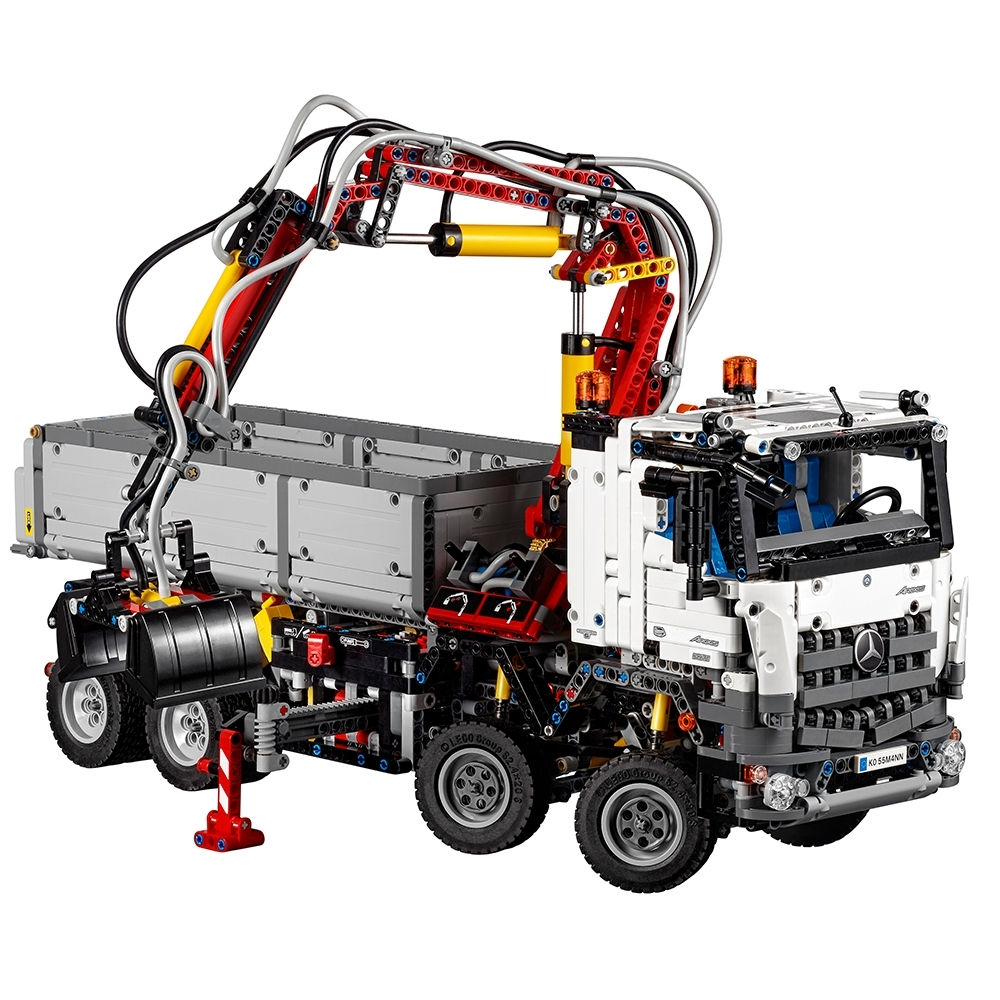
\includegraphics[trim={0 0 0 4cm},clip,width=0.85\textwidth]{2015_mercedes_arocs_42043.jpg}
\end{figure}
\end{frame}

\begin{frame}[fragile]{Instructions (484 pages, 2793 pc.)}
\begin{figure}[H]
 \centering
 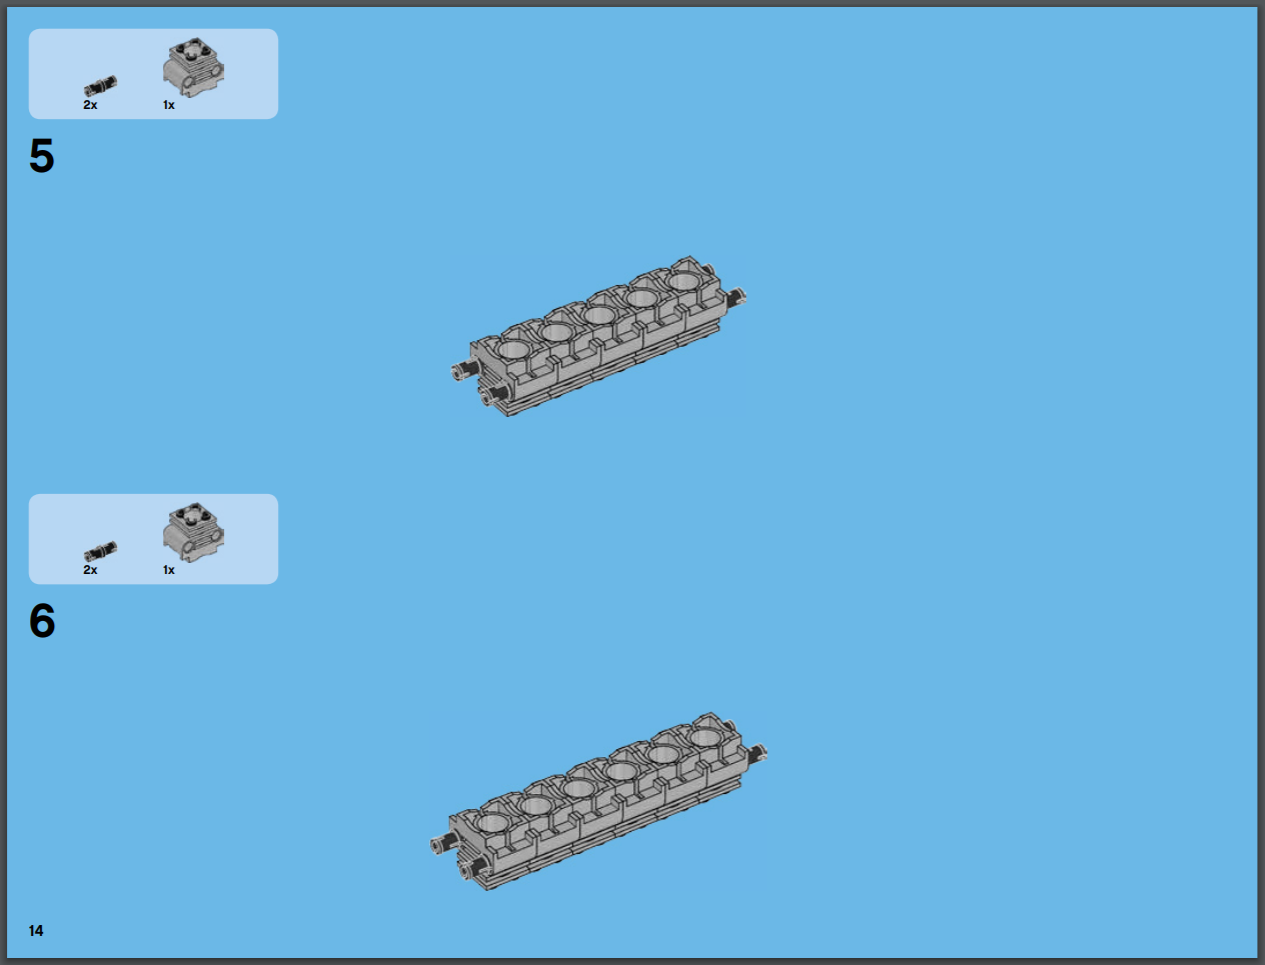
\includegraphics[width=0.8\textwidth]{2015_42043_instructions.png}
\end{figure}
\end{frame}


\begin{frame}[fragile]{}
\begin{itemize}
\item[--] Technic gets back on track, offering new versions of classic models. This time the level of sophistication is dramatically increased, along with the number of pieces. \vspace{3mm}
\item[--] With the full transition to studless beams, the models then become branded, now that styling can really capture the actual vehicle it represents. \vspace{3mm}
\item[--] However, with a return to tradition one thing remains different from early models: instructions are generally trivially easy to follow. Arguably, long term attention becomes the challenge rather than working out each step of the build. \vspace{3mm}
\end{itemize}
\end{frame}


\begin{frame}[fragile]{}
\begin{figure}[H]
 \centering
 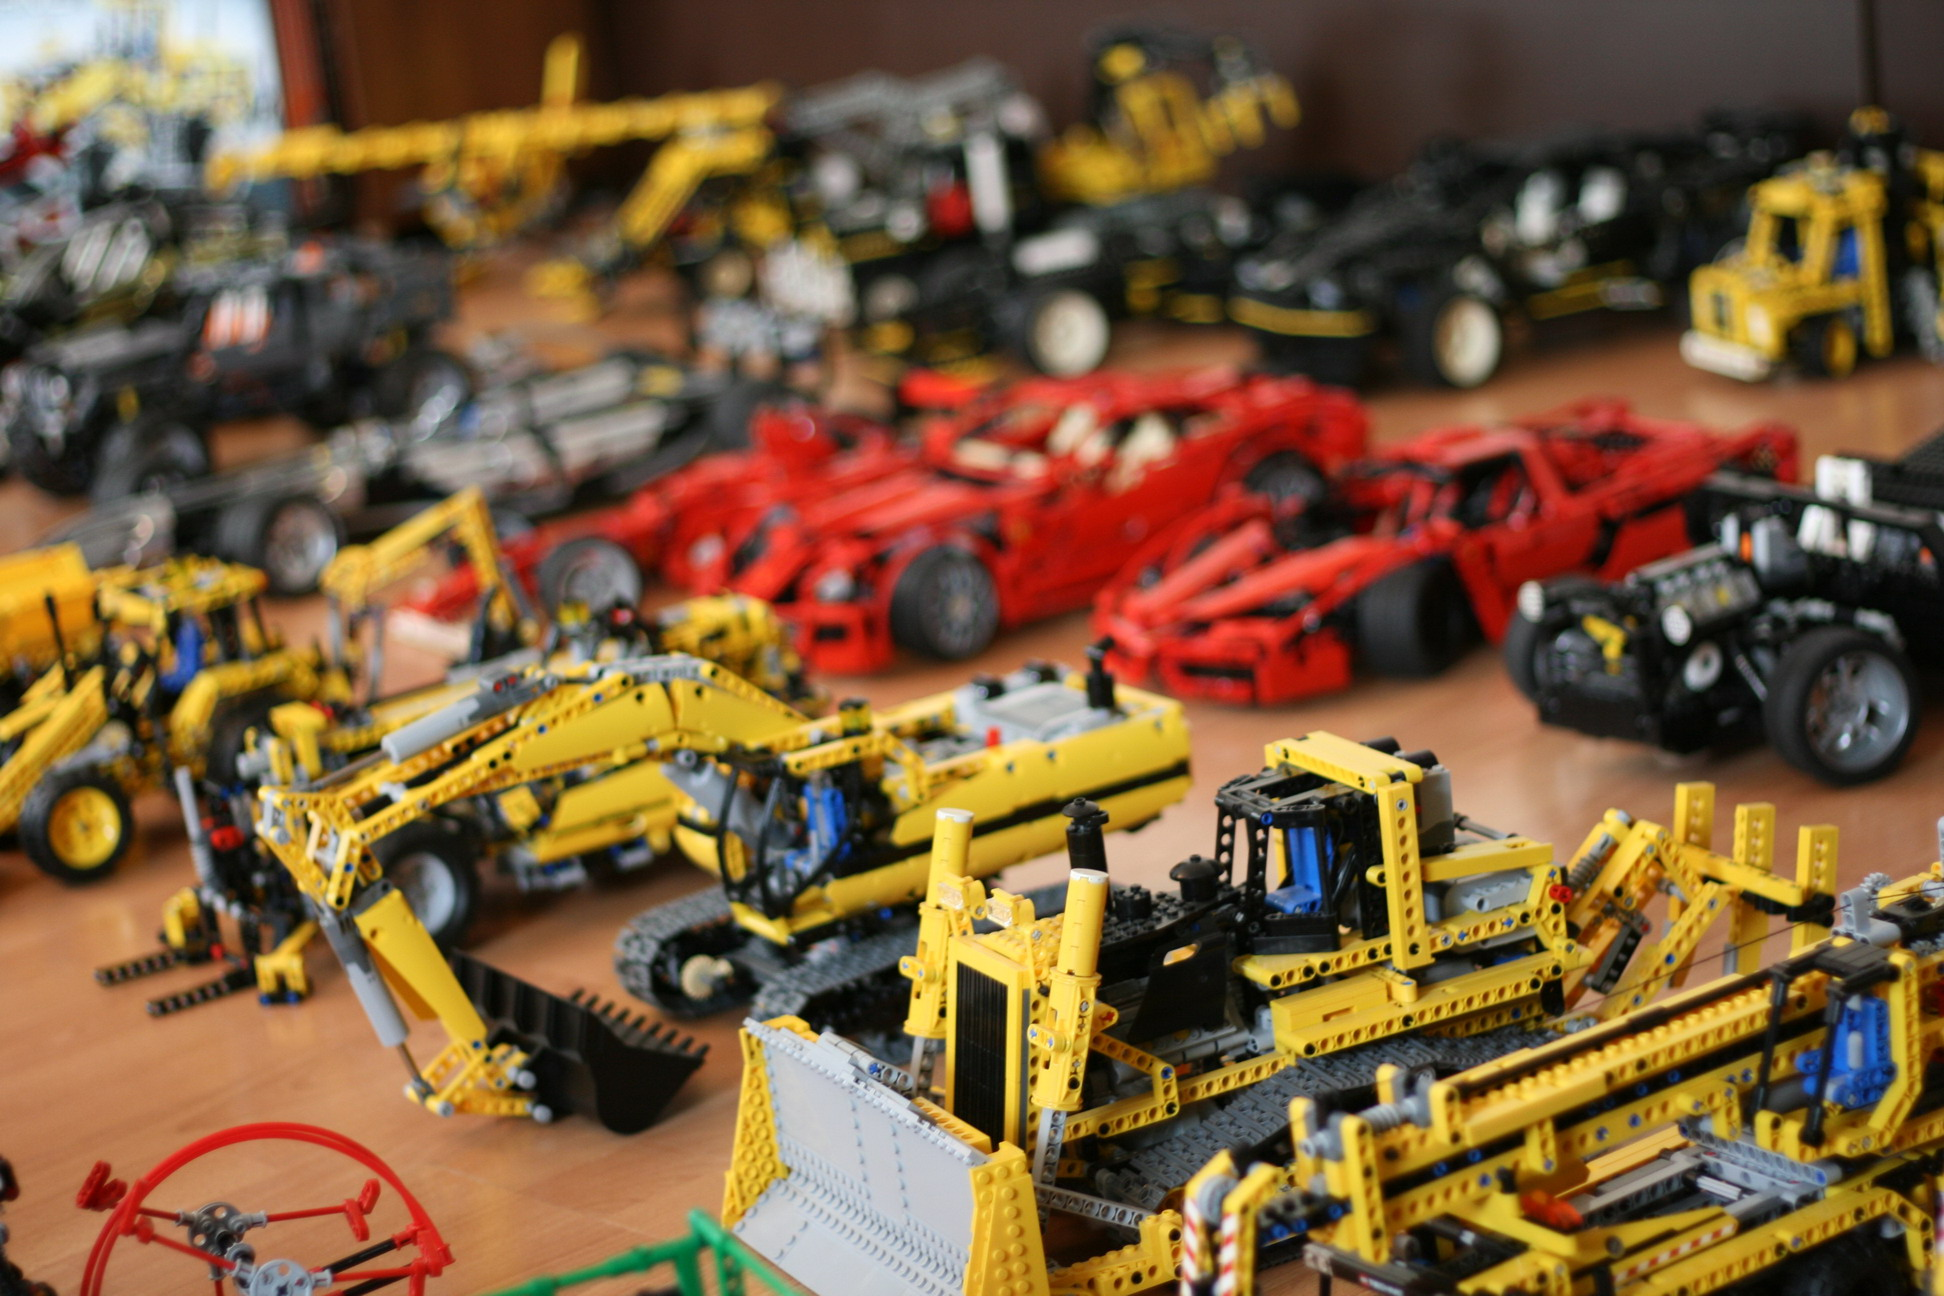
\includegraphics[width=0.99\textwidth]{0-1-lego-technic-collection-2_resize.jpg}
\end{figure}
\end{frame}


%%
\begin{frame}[plain]
  \titlepage
\end{frame}


\end{document}





%% EXTRAS


\begin{frame}[fragile]{1991: 8856 Helicopter}
\begin{figure}[H]
 \centering
 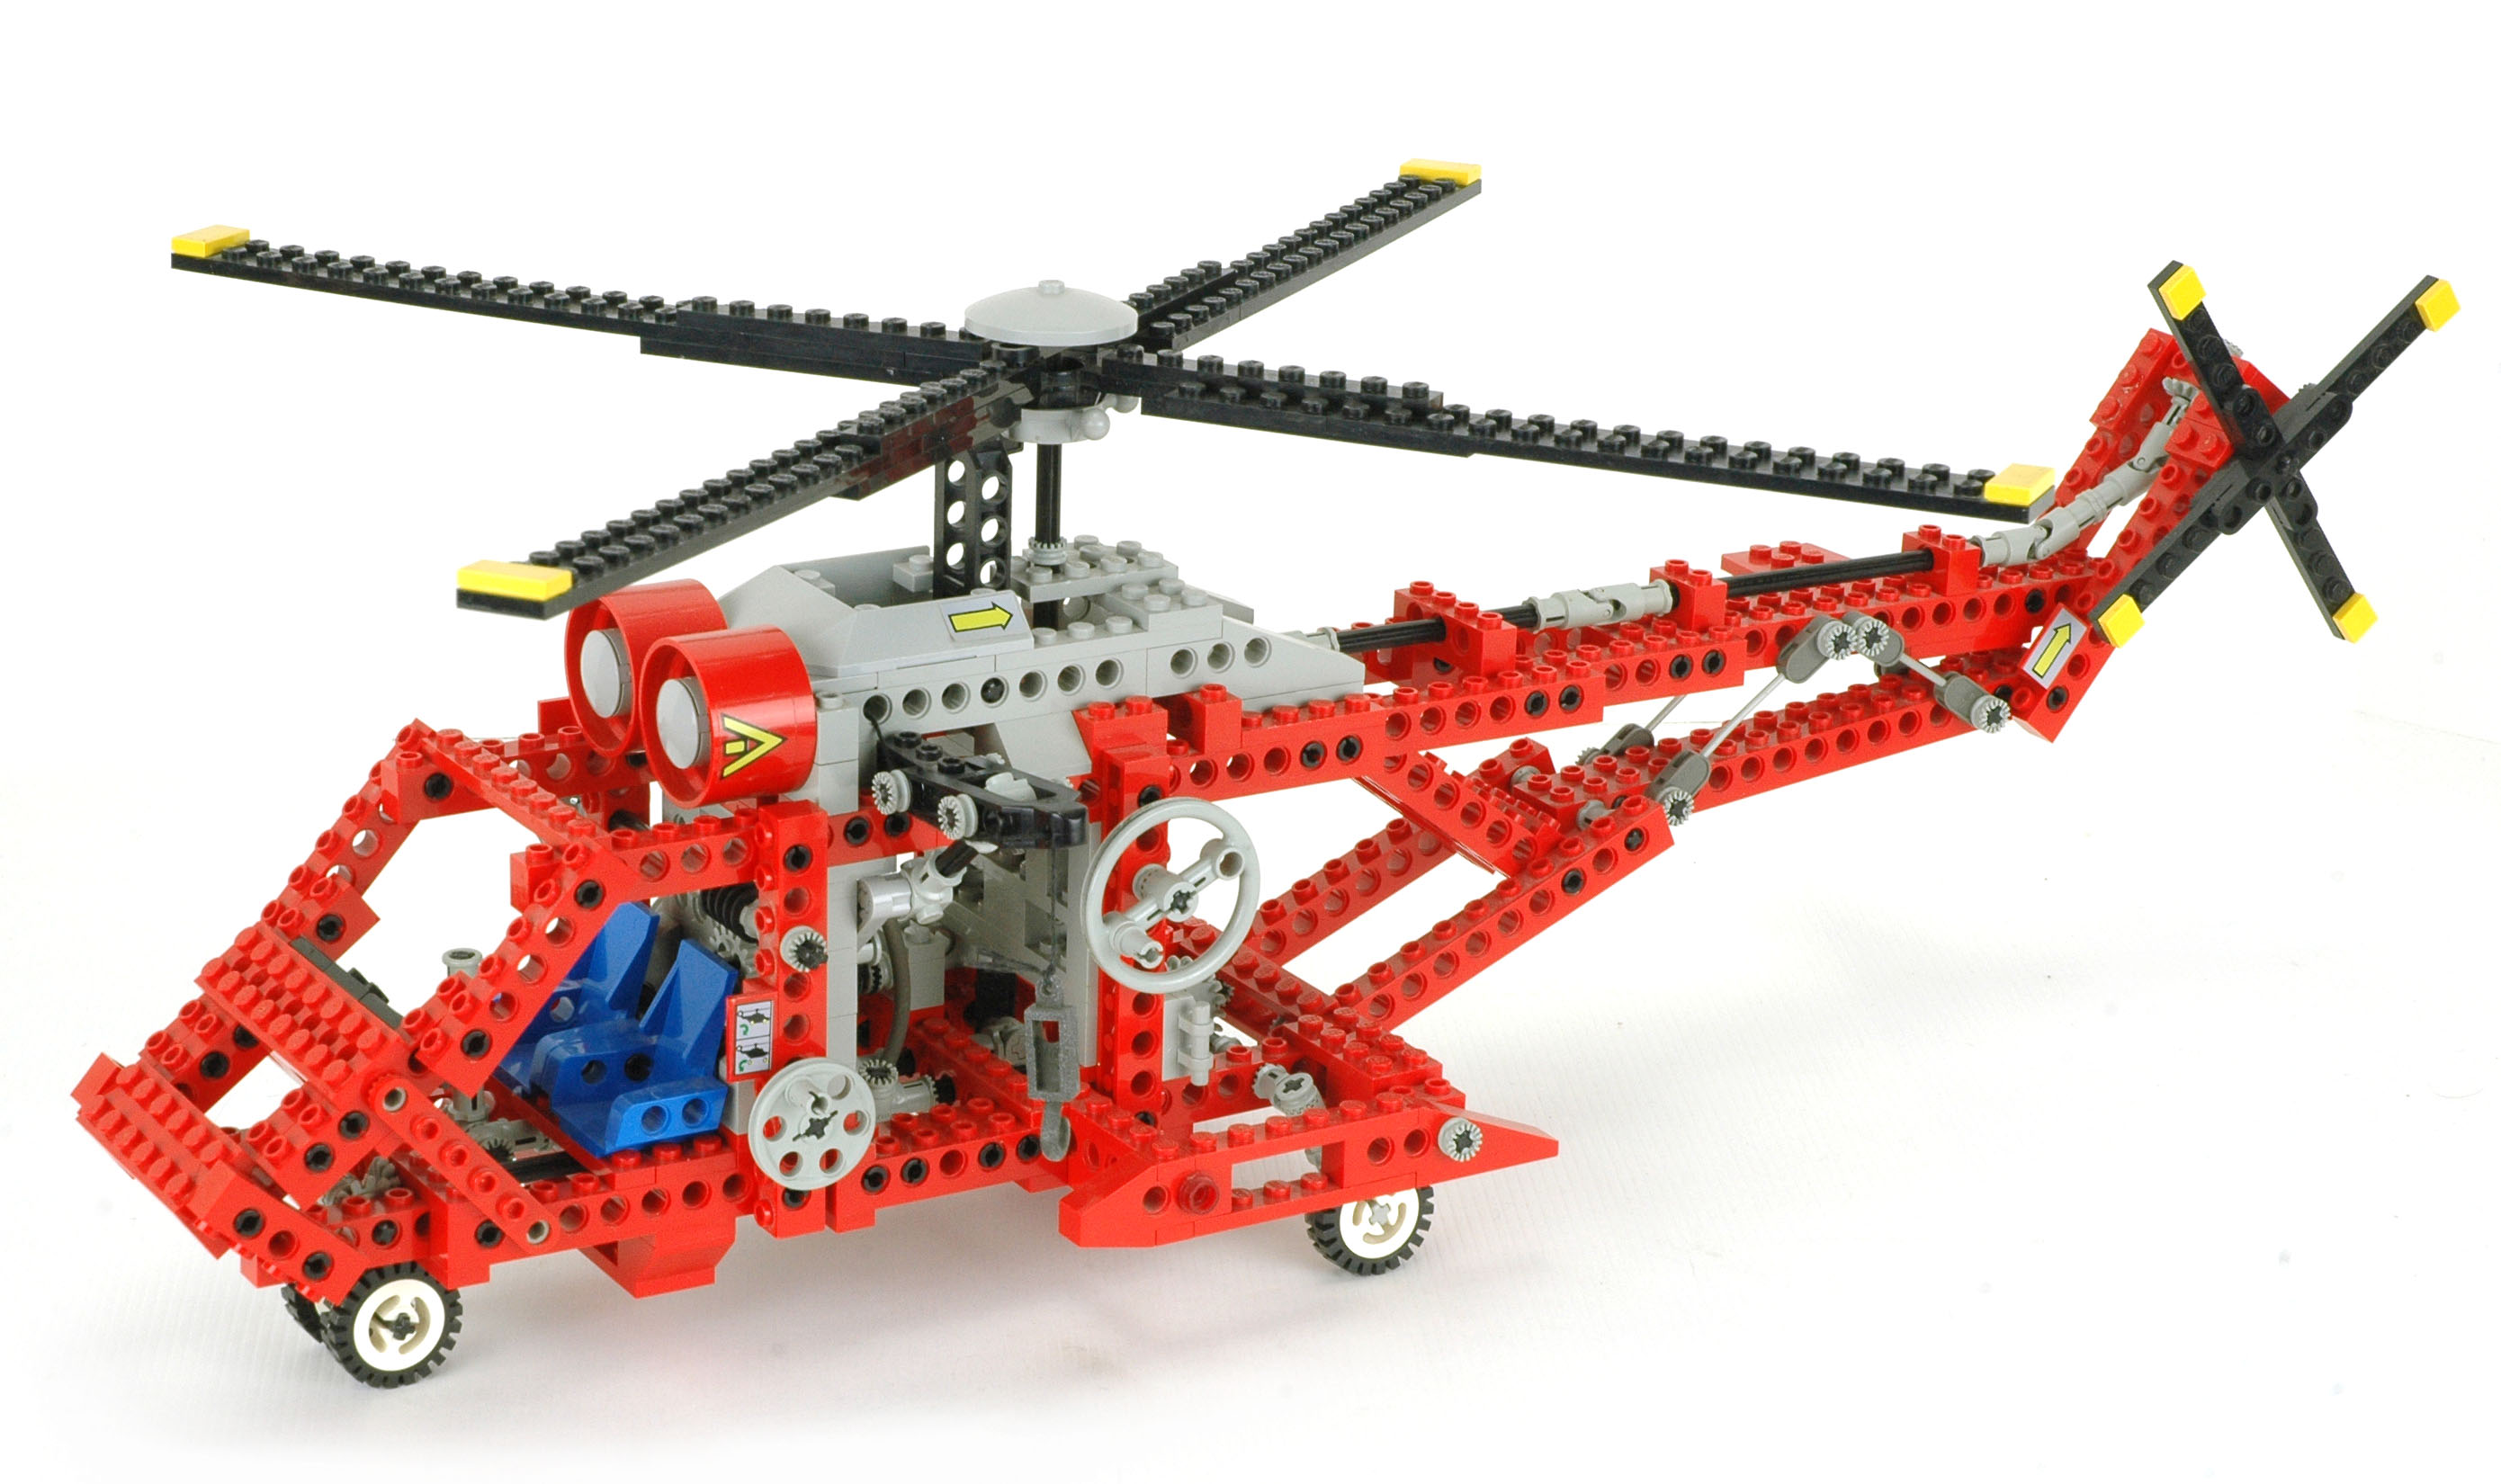
\includegraphics[width=0.99\textwidth]{1991_8856_helicopter.jpg}
\end{figure}
\end{frame}


\begin{frame}[fragile]{1980: 8700 4.5v motor set}
\begin{figure}[H]
 \centering
 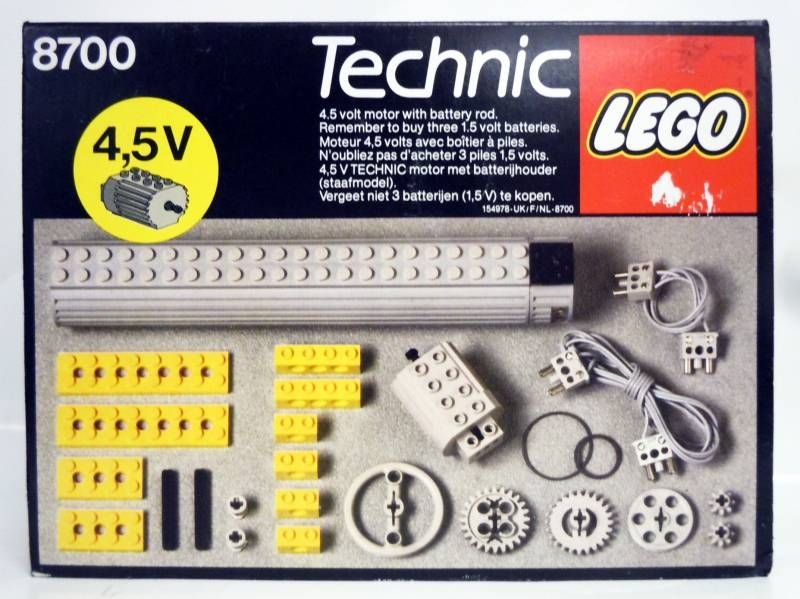
\includegraphics[width=0.9\textwidth]{1980_8700_motor}
\end{figure}
\end{frame}

\begin{frame}[fragile]{2016: Tractor}
\begin{figure}[H]
 \centering
 \includegraphics[width=0.99\textwidth]{2016_tractor_nh.jpg}
\end{figure}
\end{frame}

\begin{frame}[fragile]{2017: Excavator}
\begin{figure}[H]
 \centering
 \includegraphics[width=0.99\textwidth]{2017_excavator_nh.jpg}
\end{figure}
\end{frame}

\begin{frame}[fragile]{2017: Porsche}
\begin{figure}[H]
 \centering
 \includegraphics[width=0.99\textwidth]{2017_porsche_nh.jpg}
\end{figure}
\end{frame}

\begin{frame}[fragile]{2019: 42100 Excavator}
\begin{figure}[H]
 \centering
 \includegraphics[width=0.99\textwidth]{2019_42100_excavator.jpg}
\end{figure}
\end{frame}